\documentclass[thesis.tex]{subfiles}
 
\newcommand{\set}[1]{\mathcal {#1}}
\newcommand{\distribution}[1]{\mathcal {#1}}
\newcommand{\sized}[1]{\tilde \set {#1}}

\newcommand{\radius}{r}
\newcommand{\dist}[2]{\distf({#1},{#2})}
\newcommand{\distf}{d}
\newcommand{\diam}[1]{\textnormal{diam}({#1})}
\newcommand{\codiam}[1]{\textnormal{codiam}({#1})}
\newcommand{\aspect}[1]{\Delta_{#1}}

\newcommand{\minkdim}{\text{dim}_\textnormal{Mink}}
\newcommand{\krdim}{\text{dim}_\textnormal{exp}}
\newcommand{\doubdim}{\text{dim}_\textnormal{doub}}
\newcommand{\dualdim}{\text{dim}_{\textnormal{doub}^*}}
\newcommand{\holedim}{\text{dim}_{\textnormal{hole}}}

\newcommand{\cexp}{c_\textnormal{exp}}
\newcommand{\cdoub}{c_\textnormal{doub}}
\newcommand{\cdoubstar}{c_{\textnormal{doub}^*}}
\newcommand{\chole}{c_\textnormal{hole}}

\newcommand{\poly}[1]{\text{poly}(#1)}
\newcommand{\eann}{(1+\varepsilon)\text{-ann}}

\newcommand{\p}{\ensuremath p}
\newcommand{\q}{\ensuremath q}
%\newcommand{\varfont}[1]{\ensuremath{\textup{\text{{#1}}}}}
\newcommand{\mkfunction}[1]{\ifmmode{\textnormal{{#1}}}}
\newcommand{\level}[1]      {\mkfunction{level}({#1})}
\newcommand{\parent}[1]     {\mkfunction{parent}({#1})}
%\newcommand{\children}[1]   {\mkfunction{children}({#1})}
\newcommand{\covdist}[1]    {\mkfunction{covdist}({#1})}
\newcommand{\sepdist}[1]    {\mkfunction{sepdist}({#1})}
\newcommand{\descendants}[1]{\mkfunction{descendants}({#1})}
\newcommand{\maxdist}[1]    {\mkfunction{maxdist}({#1})}
\newcommand{\height}[1]     {\mkfunction{height}({#1})}
\newcommand{\data}[1]       {\mkfunction{data}({#1})}
\newcommand{\datapoint}[1]  {\mkfunction{dp}({#1})}
\newcommand{\nn}[1]         {\mkfunction{nn}[{#1}]}
\makeatletter
\def\nn{\@ifstar\@nn\@@nn}
\def\@nn#1{\mkfunction{nn}^*[{#1}]}
\def\@@nn#1{\mkfunction{nn}[{#1}]}
\def\children{\@ifstar\@children\@@children}
\def\@children#1{\mkfunction{children}'({#1})}
\def\@@children#1{\mkfunction{children}({#1})}
\makeatother

% FIXME: should these be changed?
\newcommand{\mergeinsert}{\mkprocedure{merge\_insert}}
\newcommand{\ctmergeloop}{\mkprocedure{merge\_loop}}
\newcommand{\findnnloop}{\mkprocedure{findnn\_loop}}
\newcommand{\findnn}{\mkprocedure{findnn}}
\newcommand{\findnnorig}{\mkprocedure{findnn\_orig}}

%\newcommand{\nn}[1]{\ensuremath{\ensuremath{{{#1}}_{nn}}}}
\newcommand{\exprad}[1]{\ensuremath{\ensuremath{2}}}
\newcommand{\pack}{\ensuremath{\textnormal{\ttfamily pack}}}
\newcommand{\rmNodes}{\ensuremath{\textnormal{\ttfamily rmNodes}}}
\newcommand{\dualnn}{\ensuremath{\textnormal{\ttfamily dualTreeNN}}}
\newcommand{\ctmerge}{\ensuremath{\textnormal{\ttfamily merge}}}
\newcommand{\ctinsert}{\ensuremath{\textnormal{\ttfamily insert}}}
\newcommand{\ctinsertloop}{\ensuremath{\textnormal{\ttfamily insert\_loop}}}
\newcommand{\ctinsertHelper}{\ensuremath{\textnormal{\text{\ttfamily insert\_loop}}}}
\newcommand{\rebalance}{\ensuremath{\textnormal{\ttfamily rebalance}}}
\newcommand{\rebalanceHelper}{\ensuremath{\textnormal{\ttfamily rebalance\_loop}}}
\newcommand{\mkvar}[1]{\ensuremath{\textnormal{\textit{{#1}}}}}
\newcommand{\nullvar}{\ensuremath{\textup{\textnormal{\ttfamily null}}}}
%\newcommand{\datapoint}[1]{\ensuremath{\textup{\textnormal{\ttfamily dp}({#1})}}}

\algnewcommand\TRUE{\textbf{true}\space}
\algnewcommand\FALSE{\textbf{false}\space}
\algnewcommand\NOT{\textbf{not}\space}

\definecolor{darkred}{rgb}{0.5,0,0}
\definecolor{lightblue}{rgb}{0.5,0.5,1}
\definecolor{colorOrig}{RGB}{102,51,0}
\definecolor{colorMlpack}{RGB}{204,153,0}

%%%%%%%%%%%%%%%%%%%%%%%%%%%%%%%%%%%%%%%%%%%%%%%%%%%%%%%%%%%%%%%%%%%%%%%%%%%%%%%%

\begin{document}
\chapter{The Cover Tree}

\noindent
The cover tree is a data structure for fast nearest neighbor queries in arbitrary metric spaces.
Cover trees were first introduced by \cite{beygelzimer2006cover},
and they have seen widespread use in the machine learning community since then.
%(See Section \ref{sec:review}.)
This chapter improves the cover tree's run time both in theory and practice.
Our first contribution is to improve the cover tree's runtime bounds.
As an example, 
the original cover tree was able to find nearest neighbors in time $O(\cexp^{12}\log n)$,
and we improve this bound to $O(\chole^4\log n)$ for i.i.d.\ data.
Here $\cexp$ and $\chole$ are measures of the ``intrinsic dimensionality'' of the data.
We will show that on typical datasets $\cexp \approx \chole$,
and we will argue that in pathological data sets $\chole$ more accurately represents our intuitive notion of dimensionality.
We further provide practical improvements to the cover tree's implementation.
Experiments show that with these improvements,
the cover tree is the fastest technique available for nearest neighbor queries on many tasks.
%The original cover tree's runtime bounds were given in terms of the expansion constant of the metric space.
%We provide a more robust analysis in terms of the doubling constant, 
%the aspect ratio, 
%and a new notion of metric dimension called the hole constant.

%and connects the cover tree to the divide and conquer framework described in Chapter 1. 
%On the theoretical side, this chapter improves the analysis of the cover tree's run times.
%The original analysis was done in terms of the 

Most work on nearest neighbor queries focuses on Euclidean space,
but a major strength of the cover tree is that it works in the more general setting of metric spaces.
Section \ref{sec:metric} formally introduces metric spaces and
their importance in machine learning.
%Section \ref{sec:metric} formally introduces metric spaces and their importance in machine learning.
Section \ref{sec:measure} then provides a mathematically detailed discussion of four measures of the ``size'' of a metric space.
%the expansion dimension,
%the doubling dimension,
%the hole dimension,
%and the aspect ratio.
These quantities are important to bound the run time of operations on the cover tree.
We review standard results that demonstrate that the expansion constant $\cexp$ is not robust to small changes in the dataset.
We then review basic properties of the more robust doubling constant.
Unfortunately, we show that the doubling constant is not suitable for measuring the difficulty of exact nearest neighbor queries because there exists a data set of size $n$ with doubling dimension 2 that requires $O(n)$ distance computations to find a nearest neighbor.
We introduce the hole constant $\chole$ as a dimension that partially captures the robustness of the doubling dimension but is suitable for bounding the runtime of exact nearest neighbor queries.
We also provide new results on the aspect ratio of a data set 
(ratio of largest to smallest distance)
that will be needed to bound the runtime of the cover tree.
%We also review properties of the aspect ratio and provide novel bounds on its size.
%The runtime of nearest neighbor queries is well known to depend on the dimension of the space,
%but the notion of dimension in a metric space is not as simple as in Euclidean space.
%Previous analysis of the cover tree was done in terms of the expansion dimension,
%which is known to be non-robust to small changes in the data set.
Section \ref{sec:review} then reviews the history of techniques for faster nearest neighbor queries.
The main theme we emphasize is that the expansion constant is widely used to bound the runtime of exact nearest neighbor queries,
and the doubling constant is widely used to bound the runtime of approximate nearest neighbor queries.

Section \ref{sec:original} formally describes the original cover tree data structure.
We use the mathematical techniques developed in previous sections to provide novel runtime bounds for querying and inserting data points.
We also provide a novel algorithm for approximate nearest neighbor queries that improves on the algorithm of \cite{beygelzimer2006cover}.
Section \ref{sec:simplified} then presents the simplified cover tree.
The simplified cover tree is more awkward to analyze theoretically but has a number of practical advantages.
In particular:
(i) the invariants are simpler;
(ii) there are fewer nodes in the tree resulting in smaller constant factors;
(iii) we introduce a new invariant that helps maintain tree balance;
(iv) we show how to make the tree cache efficient;
and (v) we show how to merge two trees together, resulting in a parallel tree construction algorithm and fast cross validation algorithm (based on the results in Chapter \ref{}).
Finally, Section \ref{sec:experiments} concludes with a series of five experiments.
We use benchmark datasets with the Euclidean distance to show that our simplified cover tree implementation is faster than both existing cover tree implementations and other techniques specialized for Euclidean distance nearest neighbor queries.
We also compare the simplified and original cover trees on non-Euclidean protein interaction and computer vision problems.

%A key difficulty when generalizing from Euclidean space to metric space is that the notion of dimension is no longer straightforward.
%The runtime of nearest neighbor queries in Euclidean space is well known to depend on the dimensionality of the data.
%Section \ref{sec:measure} reviews several competing measures of dimension.
%Section \ref{sec:review} reviews the existing techniques for faster nearest neighbor queries.
%Section \ref{sec:original} formally describes the original cover tree data structure.
%Section \ref{sec:simplified} presents the simplified cover tree heuristic.
%Section \ref{sec:experiments} concludes the chapter with experiments demonstrating the improvements success in practice.

%\noindent
%Data structures for fast nearest neighbor queries are a fundamental algorithmic tool.
%In machine learning, 
%these spacial data structures are most commonly used to speed up $k$-nearest neighbor classification.
%The $k$d-tree \cite{friedman1977} is probably the most famous of these structures,
%but it is limited to only Euclidean space.
%
%
%These data structures are most often used to speed up the $k$-nearest neighbor classification algorithm.
%But many other learning tasks also require neighbor searches,
%and cover trees can speed up these tasks as well:
%localized support vector machines \cite{Segata2010},
%dimensionality reduction \cite{Lisitsyn2013},
%and reinforcement learning \cite{Tziortziotis2014}.
%Making cover trees faster---the main contribution of this paper---also makes these other tasks faster.
%
%Nearest neighbor queries are a fundamental algorithmic tool,
%and speeding up nearest neighbor queries makes many algorithms faster.
%It is simple and effective in practice,
%but it can only be used on Euclidean spaces.
%
%

%%%%%%%%%%%%%%%%%%%%%%%%%%%%%%%%%%%%%%%%%%%%%%%%%%%%%%%%%%%%%%%%%%%%%%%%%%%%%%%%

\section{Definitions}
\label{sec:metric}

This section first defines metric spaces and the nearest neighbor problem.
%Then it shows motivating examples of useful metric spaces in machine learning.
%
A set $\set X$ equipped with a distance function $\distf : \set X \times \set X \to \R$ is a \defn{metric space} if it obeys the following three properties:
\begin{enumerate}
    %\item \defn{Non-negativity}.  For all $x_1,x_2\in\set X$, $\dist{x_1}{x_2} \ge 0$.
    \item \defn{Indiscernability}.  For all $x_1,x_2\in\set X$, $\dist{x_1}{x_2} = 0$ if and only if $x_1=x_2$.
    \item \defn{Symmetry}. For all $x_1,x_2\in\set X$, $\dist{x_1}{x_2} = \dist{x_2}{x_2}$.
    \item \defn{Triangle inequality}.  For all $x_1,x_2,x_3\in\set X$, $\dist{x_1}{x_2} + \dist{x_2}{x_3}\ge\dist{x_1}{x_3}$.
\end{enumerate}
We will use the script $\set X$ notation for metric spaces that may be either infinite or finite,
and the plain $X$ for metric spaces that must be finite.
In particular, $X$ will typically denote a data set sampled from some larger space $\set X$,
as in the following definition of the nearest neighbor problem.
%A basic property of metric spaces is that if $\set X$ is a metric space,
%then any $\set X' \subseteq\set X$ is also a metric space with the same distance function.
%Therefore, if we have a data set $X$ sampled from some metric space $\set X$,
%we will refer 
%Therefore, we will often refer to subsets of metric spaces as metric spaces without loss of generality.
%We will use the script notation $\set X$ for possibly infinite metrics,

Let $\set X$ be a metric space, $X\subset\set X$, and $x$ be in $\set X$ but not $X$.
We call a point $y^*\in X$ a \defn{nearest neighbor} of $x$ if it is contained in $\argmin_{y\in X} \dist{x}{y}$.
In most cases $y^*$ will be unique 
(so we will often refer to \textit{the} nearest neighbor of $x$).
For all $\varepsilon \ge 0$,
we call a point $\hat y$ a \defn{$(1+\varepsilon)$-approximate nearest neighbor} (\defn{ann}) of $x$ if $\hat y$ satisfies $\dist{x}{\hat y} \le (1+\varepsilon) \cdot\dist{x}{y^*}$.
In particular, if $\hat y$ is a 1-ann, then $\hat y$ is a nearest neighbor.

%\subsection{Metric learning}

%In nearest neighbor classification,
%
%\cite{kulis2013metric} and \cite{bellet2013survey} provide tutorials.

%\begin{table}[H]
    %\small
    %\centering
    %\begin{tabular}{lccc}
        %\toprule
        %\vspace{-0.25in}
        %&~\hspace{1.2in}~&~\hspace{1.2in}~&~\hspace{1.2in}~\\
        %data structure & space & find nearest neighbor & insertion \\
        %\midrule
        %ball tree \cite{} & $O(n)$ & $O(n)$ & $O(n)$ \\
        %metric skip list \cite{karger2002finding} & $O(n\log n)$ & $\cexp{}^{O(1)}\log n$ & $\cexp^{O(1)}\log n\log\log n$ \\
        %navigating net \cite{} & $O(n)$ \\
        %cover tree \cite{} & $O(n)$ & $O(\cexp^8\log n)$ & $O(\cexp^{12}\log n)$ \\
        %simplified cover tree & $O(n)$ & $O(\cdoub{}\log \aspect{})$ \\
                              %&        & $O(\cdoub{}\log n)$ \\
        %\bottomrule
    %\end{tabular}
    %%\end{tabularx}
    %\caption{
        %Summary of the runtime and space usage of several nearest neighbor data structures.
        %Here $n$ represents the size of the dataset.
    %}
%\end{table}

%%%%%%%%%%%%%%%%%%%%%%%%%%%%%%%%%%%%%%%%%%%%%%%%%%%%%%%%%%%%%%%%%%%%%%%%%%%%%%%%

\section{Measuring the size of a metric space}
\label{sec:measure}

The runtime of nearest neighbor queries depends on the dimension of the data,
and there are many ways to define the dimension of arbitrary metric spaces.
The expansion and doubling dimensions are the two most popular. 
The expansion dimension can be used to bound the runtime of either exact or approximate nearest neighbor queries,
but it is not robust to small changes in the data.
This lack of robustness can make runtime bounds based on the expansion dimension trivial 
(i.e.\ linear).
On the other hand, 
the doubling dimension can only be used to bound the runtime of approximate nearest neighbor queries,
but it is more robust than the expansion dimension.
Therefore bounds using the doubling dimension are stronger than those using the expansion dimension.
The original runtime bounds for the cover tree were in terms of the expansion dimension,
but Section \ref{sec:original} will improve these bounds to use the doubling dimension in the case of approximate nearest neighbor searches.
This section begins with a detailed discussion of these two dimensions, 
including important lemmas used in the proofs in Section \ref{sec:original}.
Then we introduce a novel third dimension called the hole dimension.
We show in this section that the hole dimension is more robust than the expansion dimension,
and in Section \ref{sec:original} the hole dimension is used to bound the runtime of exact nearest neighbor queries.
This section concludes with a discussion of the aspect ratio of a metric space.
The log of the aspect ration will bound the height of the cover tree (Lemma \ref{lemma:height} in Section \ref{sec:original}).
%Lemma \ref{lemma:height} in Section \ref{sec:original} shows that the log of the aspect ratio bounds the height of the cover tree.
In this section, we provide a novel bound showing that under mild regularity conditions the aspect ratio of i.i.d.\ data is $O(n^3)$, 
and thus the height of the cover tree is $O(\log n)$.
No existing results show that the cover tree is well-balanced in this way.

%doubling constant $\cdoub$, 
%the hole constant $\chole$,
%and the aspect ratio $\aspect{}$.
%Previous analysis of the cover tree relied only on the expansion constant.
%As we shall see, the expansion constant is not a robust measure of difficulty for nearest neighbor queries.
%The doubling constant is significantly more robust,
%however it is only suitable for measuring the difficulty of approximate nearest neighbor queries.
%The hole constant is a no
%The analysis in Section \ref{}instead use the hole constant and aspect ratio.
%In this section, we will formally define these constants and present their basic properties.
%In particular, we will see that the doubling constant and aspect ratio are more robust measures of size than the expansion constant.

%%%%%%%%%%%%%%%%%%%%%%%%%%%%%%%%%%%%%%%%

\subsection{Expansion dimension}

The expansion dimension is the only notion of dimensionality that has been used for bounding the runtime of exact nearest neighbor queries.
It was introduced by
\citet{karger2002finding},
and was subsequently used in
\citet{krauthgamer2004navigating},
\citet{beygelzimer2006cover},
\citet{ram2009linear},
and \citet{curtin2015plug}.
In this section, we define the expansion constant and show that it is not a robust measure of a metric's dimension.

Throughout this section we will work with the metric space $(\set X,d)$
where the set $\set X$ may be either finite or infinite.
We let $B(x,\delta)$ denote the \defn{ball} centered around $x$ of radius $\delta$. 
That is,
\begin{equation}
    B(x,\delta) = \{ x' : x'\in\set X, \dist{x}{x'} \le \delta \}.
\end{equation}
The expansion dimension of a metric is only valid for metrics that also have a notion of volume,
which is given by the function $\mu : \{\set X\} \to \R^+$.% 
\footnote{
    Formally, $\mu$ is a measure and $\{\set X\}$ is a $\sigma$-algebra on $\set X$.
    Since we are primarily interested in the properties of finite sets,
    we will not need to formally use measure theory.
}
In finite metric spaces, $\mu X$ is defined to be the number of points in $X$.
In the Euclidean space $\set X=\R^d$, $\mu$ is defined to be the standard Euclidean volume,
and in particular $\mu B(x,\delta) = \Theta(\delta^d)$.

The \defn{expansion dimension} of a metric space $\set X$ is defined as
\begin{equation}
    \krdim = \log_2 \cexp
    ,
\end{equation}
where $\cexp$ is called the \defn{expansion constant} and defined as
\begin{equation}
    \cexp = \max_{x\in\set X, \delta\in\R^+} \frac{\mu B(x,2\delta)}{\mu B(x,\delta)}
    .
\end{equation}
In words, the expansion dimension measures how the volume of a ball changes as you increase the radius.
The intuition behind why this is a good notion of a metric's dimension is that it agrees with the standard dimension in Euclidean space.
This is shown formally in the following standard lemma.
\begin{lemma}
    \label{lemma:expansionEuclidean}
    Let $\set X=\R^d$ with the standard $L_2$ distance function.
    Then $\krdim\set X=\Theta(d)$.
\end{lemma}
\begin{proof}[Proof (sketch)]
    The volume of a Euclidean ball with radius $\delta$ is $\Theta(\delta^d)$.
    The expansion constant is the maximum of the ratio $\mu B(x,2\delta) / \mu B (x,\delta)$.
    In Euclidean space this ratio is independent of $x$ and $\delta$.
    Letting $\delta=1$ gives the ratio is $\mu B(x,2) / \mu B(x,1) = \Theta(2^d)$.
    Taking the log gives that $\krdim\set X = \Theta(d)$.
\end{proof}

\noindent
Unfortunately, the expansion dimension is known to have many defects which make runtime bounds less useful.
The algorithmic consequence of these defects is that runtime bounds based on the expansion dimension are often trivial.

\begin{example}
    A subset of a metric space may have arbitrarily large expansion dimension compared to the host space.
    \fixme{}
\end{example}

\begin{example}
    Adding a single point to a space may change the expansion dimension by an arbitrary amount.
    \fixme{}
\end{example}

%%%%%%%%%%%%%%%%%%%%%%%%%%%%%%%%%%%%%%%%

\subsection{Doubling dimension}

The doubling dimension is more robust than the expansion dimension,
but cannot be used to provide non-trivial runtime bounds for exact nearest neighbor queries (see Theorem \ref{theorem:exactdoubling} below).
It has, however, seen widespread application in bounding the runtime of approximate nearest neighbor queries.
\cite{krauthgamer2005black} showed that the doubling constant is the correct way to measure the difficulty of $\eann$ queries in the following sense:
a $\eann$ query can be answered in polylogarithmic time using polynomial space if and only if $\cdoub = O(\log n)$.
No similar result pairing exact nearest neighbor queries to a metric dimension is known.

The doubling dimension is widely used in computer science and mathematics.
Before formally defining it, we briefly review these many uses. 
The term doubling dimension was first used by \citet{gupta2003bounded} in their study of low dimensional embeddings for nearest neighbor queries,
but the main idea was introduced by \citet{assoud1979etude} to study fractals.%
\footnote{
    There are many terms in the literature with essentially the same meaning as the doubling dimension.
    For example, the terms Assoud dimension and Minkowski dimensions are both used in fractal geometry;
    and the terms covering number, packing number, $\varepsilon$-nets, and metric entropy are all used in computer science. 
}
%The doubling dimension is more robust than the expansion dimension,
%so runtime bounds in terms of the doubling dimension are more useful. 
%Unfortunately, they are harder to prove.
%Theorem \ref{} at the end of this section shows the novel result that there is no efficient data structure for exact nearest neighbor queries even in metrics with low doubling dimension.
In the context of machine learning, the doubling dimension has found use both statistically and algorithmically.
Statistically, the doubling dimension is a standard tool for proving regret bounds.
For example, \citet{luxburg2004distance} uses the doubling dimension to provide the first large margin bounds for classifiers in metric spaces,
and Chapter 27 of \cite{shalev2014understanding} shows how to bound the Rademacher complexity of a classifier using the doubling dimension.
A particularly apropos work in this vein is \citet{kontorovich2015bayes},
which uses the doubling dimension to derive the first Bayes-consistent 1-nearest neighbor algorithm.
Algorithmically, the doubling dimension is used to develop approximation algorithms.
Chapter 32 of \cite{toth2017handbook} provides a survey of how the doubling dimension is used to approximate a variety of NP-hard problems.
In the context of machine learning, \citet{gottlieb2014near} shows the first approximation algorithm for sample compression,
and
\citet{gottlieb2014efficient} and \citet{gottlieb2017efficient} both create efficiently realizable approximation algorithms for classification in metric spaces.
%Little recent work on nearest neighbor data structures has used doubling dimension.
%The only examples known to the author are \citet{clarkson1997nearest}\footnote{Clarkson refers to the doubling dimension by an essentially equivalent concept he calls the $\gamma$-dominator bound.} and \citet{krauthgamer2004navigating}.
%Theorem \ref{} at the end of this section may explain why.


The doubling dimension is closely related to the ideas of covering and packing numbers,
so we introduce these ideas first.
A \defn{$\delta$-covering} of a metric space $\set X$ is a set $\{x_1,x_2,...,x_n\} \subseteq \set X$ such that for all $x\in\set X$, there exists an $x_i$ such that $\dist{x}{x_i} < \delta$.
The \defn{$\delta$-covering number} $N_\delta(\set X)$ is the cardinality of the smallest $\delta$-covering.
%The log of the covering number $\log N_\delta(\set X)$ is called the \defn{metric entropy} of $\set X$.
A \defn{$\delta$-packing} of a metric space $\set X$ is a set $\{x_1,x_2,...,x_M\} \subseteq \set X$ such that $\dist{x_i}{x_j} > \delta$ for all $i \ne j$.
The \defn{$\delta$-packing number} $M_\delta (\set X)$ is the cardinality of the largest $\delta$-packing.
The covering number and packing number of a set are closely related.
We will make heavy use of the following standard lemma in the analysis of the cover tree.

\begin{lemma}
    \label{lemma:coverpacking}
    For any metric space $\set X$ and any $\delta>0$,
    %$M_{2\delta}(\set X) \le N_\delta(\set X) \le M_{\delta}(\set X)$.
    \begin{equation}
        M_{2\delta}(\set X) \le N_\delta(\set X) \le M_{\delta}(\set X)
        .
    \end{equation}
\end{lemma}
\begin{proof}
    To prove the first inequality, let $P$ be a $2\delta$-packing and $C$ be a $\delta$-cover of $\set X$.
    For every point $p\in P$, there must exist a $c\in C$ such that $\dist{p}{c}\le\delta$.
    No other $p'\in P$ can also satisfy $\dist{p'}{c}\le\delta$, because then by the triangle inequality
    \begin{equation}
        \dist{p'}{p} \le \dist{p'}{c}+\dist{p}{c} \le 2\delta
        ,
    \end{equation}
    which would contradict that $P$ is a $2\delta$-packing.
    In other words, for each $c\in C$, there is at most one $p\in P$.
    So $N_\delta \ge |C| \ge |P| \ge M_{2\delta}$.

    To prove the second inequality, let $\set X'\subseteq \set X$ be a maximal $\delta$-packing.
    Then there does not exist an $x\in\set X$ such that for all $x'\in\set X'$, 
    $\dist{x}{x'} > \delta$.
    (Otherwise, $\set X' \cup \{x\}$ would be a packing larger than $\set X'$.)
    Hence, $\set X'$ is also a $\delta$-cover,
    and the smallest $\delta$-cover can be no larger.
\end{proof}

%\cite{nickl2007bracketing} uses metric entropy to prove a version of the central limit theorem.
%
%\begin{example}
%\end{example}

%\begin{definition}
    %The Minkowski dimension of a metric space is defined to be
    %\begin{equation}
        %\minkdim \set X = \lim_{\delta\to0} \frac{\log N_\delta(\set X)}{\log 1/\delta}
        %.
    %\end{equation}
%\end{definition}
%
%\begin{example}
    %Let $\set X$ be a finite metric space.
    %Then $\minkdim \set X = 0$.
%\end{example}

The \defn{doubling dimension} of a metric space $\set X$ is defined to be
\begin{equation}
    \doubdim = \log_2 \cdoub
    ,
\end{equation}
where $\cdoub$ is called the \defn{doubling constant} and is defined to be
\begin{equation}
    \cdoub = \max_{x\in\set X, \radius\in\R^+} N_\radius(B_{\set X}(x,2\radius))
    .
\end{equation}
Whereas the expansion dimension measures how the volume of a ball changes as the radius changes,
the doubling dimension measures how the packing number of a ball changes.
%This minor change makes the doubling dimension more robust.
%This minor change fixes many of the problems with the doubling dimension.
%As with the expansion dimension, the doubling dimension is good notion of a metric's dimension because it agrees with the standard dimension on Euclidean space:
The following lemma shows that the doubling dimension (like the expansion dimension) agrees with the dimension in Euclidean space.
\begin{lemma}
    \label{lemma:doubleEuclidean}
    Let $\set X=\R^d$ with the standard $L_2$ distance function.
    Then $\doubdim\set X=\Theta(d)$.
\end{lemma}
\begin{proof}[Proof (sketch)]
    Follows by direct calculation as in Lemma \ref{lemma:expansionEuclidean}.
\end{proof}
\noindent
%The proof of Lemma \ref{lemma:doubleEuclidean} follows by an explicit calculation of the volume of a ball in $\mathbb{R}^d$.
%The proof is not especially interesting, and so is omitted.
The major advantage of the doubling dimension over the expansion dimension is its robustness,
as shown in the following two standard lemmas.

%%%%%%%%%%%%%%%%%%%%

\begin{lemma}
    Let $\set X$ be a metric space, and $X\subset\set X$.
    Then,
    \begin{equation}
        \label{eq:cdoubinclusion}
        %\doubdim\set X \ge \doubdim X,
        \cdoub X \le \cdoub \set X.
    \end{equation}
\end{lemma}

\begin{proof}
    \fixme{}
    %To prove \eqref{eq:cdoubinclusion},
    %let $x$ be a point in $\set X$ and $\delta\in\mathbb R^+$.
    %Then any valid $\delta$-packing of $B_{\set X_1}(x,2\delta)$ is also a valid $\delta$-packing of $B_{\set X_2}(x,2\delta)$.
%
\end{proof}

\begin{lemma}
    Let $\set X$ be a metric space, $X\subset\set X$, and $x\in\set X$.
    Then,
    \begin{equation}
        \label{eq:cdoubplusone}
        \cdoub (X\cup\{x\}) \le \cdoub X + 1.
    \end{equation}
\end{lemma}
\begin{proof}
    Let $y\in X$ and $\delta>0$.
    Let $C$ be a minimal $\delta$-covering of $B_X(y,\delta)$.
    Then the set $C\cup\{x\}$ must be a $\delta$-covering for $B_{X\cup\{x\}}(y,\delta)$.
    %So we have that $N_\delta(B_X(y,\delta)) \le N_\delta(B_{X\cup\{x\}}(y,\delta))+1$ for any $y\in X$ and $\delta>0$.
    So we have that 
    \begin{equation}
        N_\delta(B_X(y,\delta)) \le N_\delta(B_{X\cup\{x\}}(y,\delta))+1
        .
    \end{equation}
    Taking the maximum of both sides with respect to $y$ and $\delta$ gives \eqref{eq:cdoubplusone}.
    %for any $y\in X$ and $\delta>0$.
    %let $p$ be a maximal $\delta$-packing of $\set X$.
    %Assume for contradiction that there exists a $\delta$-packing $p'$ of $\set X\cup\{x\}$ such that $|p'| > |p| + 1$.
    %If $x\not\in p'$, then $p'$ is a $\delta$-packing of $\set X$.
    %But $|p'| > |p|$, which violates the assumption that $p$ is maximal.
    %If $x\in p$, then the set $p'-\{x\}$ is a packing of $\set X$.
\end{proof}

%%%%%%%%%%%%%%%%%%%%

\noindent
\citet{gupta2003bounded} and \cite{krauthgamer2004navigating} provide the following lemma relating the size of the expansion and doubling dimensions.

\begin{lemma}
    Every finite metric $(\set X,d)$ satisfies
    $\cdoub \le \cexp^4$.
    %\begin{equation}
        %\doubdim\set X \le 4\cdot\krdim\set X
        %.
    %\end{equation}
\end{lemma}
\begin{proof}
    Fix some ball $B(x,\delta)$.
    We will show that $B(x,\delta)$ can be covered by $\cexp^4$ balls of radius $\delta$.
    Let $Y$ be a $\delta$-cover of $B(x,2\delta)$.
    Then,
    \begin{equation}
        B(x,2\delta) 
        \subseteq 
        \bigcup\limits_{y\in Y} B(y,\delta) 
        \subseteq
        B(x,4\delta)
        %~~~~~
        %\text{and}
        %~~~~~
    \end{equation}
    Also, for every $y\in Y$,
    \begin{equation}
        |B(x,4\delta)| 
        \le 
        |B(y,8\delta)| 
        \le 
        \cexp^4 |B(y,\delta/2)|
        .
    \end{equation}
    We also have that $|B(y,\delta/2)|=1$.
\end{proof}

\noindent
This lemma can be used to convert runtime bounds using the doubling dimension into bounds using the expansion dimension.
We will not need to directly appeal to this lemma in our proofs.
The following theorem shows that the doubling dimension is not suitable for bounding the runtime of exact nearest neighbor queries.

\begin{theorem}
    \label{theorem:exactdoubling}
    There exists an $n$-point metric with doubling constant $\cdoub=O(1)$ such that answering exact nearest neighbor queries takes time $O(n)$.
\end{theorem}

\begin{proof}[Proof (sketch)]
    Take $n$ points arranged in a circle in $\R^2$, and let the query point $x$ be the center of the circle. 
        Select one point $y$ and reduce the distance from $x$ to $y$ by some small value $\epsilon$, leaving all other values constant.
        The resulting distance is non-Euclidean, but still satisfies the requirements of a metric space.
        There is no way to tell which point $y$ was modified in this way without checking all the points,
        thus the worst case nearest neighbor runtime is $O(n)$.
\fixme{more formality/discussion}
\end{proof}

%%%%%%%%%%%%%%%%%%%%%%%%%%%%%%%%%%%%%%%%

\subsection{Hole dimension}

The hole dimension is a novel measure of a set's dimensionality suitable for measuring the complexity of exact nearest neighbor queries.
The \defn{hole number} is defined as
\begin{align}
    \label{eq:chole}
    \chole
    = 
    &\max_{x\in\set X, \epsilon \ge 0, \delta > 0} 
    N_\delta\big( B(x,\epsilon+2\delta) \setminus B(x,\epsilon+\delta) \big)
    \\
    &
    ~~~~~~\text{s.t.}
    ~~
    B(x,\epsilon+\delta) \setminus B(x,\delta) = \{\}
    .
\end{align}
The \defn{hole dimension} is
\begin{align}
    \holedim = \log_2 \chole
    .
\end{align}

\begin{lemma}
    \label{lemma:chole}
    For any finite metric space,
    %\begin{equation}
        $\cdoub \le \chole + 1$.
    %\end{equation}
\end{lemma}

\begin{proof}
    The inequality is tight when $\epsilon=0$ in \eqref{eq:chole}.
\end{proof}

\fixme{more discussion}

%%%%%%%%%%%%%%%%%%%%%%%%%%%%%%%%%%%%%%%%

\subsection{Aspect ratio}

Unlike the expansion, doubling, and hole constants,
the aspect ratio should not be thought of as a measure of dimension.
This is because the aspect ratio is only applicable to finite sets.
Instead, it should be thought of as a measure of how evenly spread the points in a metric space are.
We will use the aspect ratio to bound the depth of the cover tree.

The \defn{diameter} of $\set X$ is the maximum distance between any two points.
In notation,
\begin{equation}
    \diam {\set X} = \max_{x_1,x_2\in\set X} \dist{x_1}{x_2}
    .
\end{equation}
The \defn{codiameter} of $\set X$ is the minimum distance between any two points.
In notation,
\begin{equation}
    \codiam {\set X} = \min_{x_1 \ne x_2\in\set X} \dist{x_1}{x_2}
    .
\end{equation}
The \defn{aspect ratio} of $\set X$, denoted by $\aspect{\set X}$, 
is the ratio of the diameter to the codiameter.
Sets with small aspect ratio are called \defn{fat},
and sets with large aspect ratio are called \defn{skinny}.

There is little necessary relationship between the aspect ratio and the inherent dimension of a space.
We emphasize this point with three examples.

\begin{example}
    Let $\set Y=\{y_1,...,y_n\}$ be the discrete metric space of size $n$;
    that is,
    \begin{equation}
        \dist{y_i}{y_j}=
        \begin{cases}
            0 & i = j \\
            1 & \text{otherwise}
        \end{cases}
        .
    \end{equation}
    Then the aspect ratio of $\set Y$ is 1 (i.e.\ as small as possible),
    and both the expansion and doubling constants of $\set Y$ are $n-1$ (i.e. arbitrarily large).
\end{example}

\begin{example}
    Now construct the set $\set Y'=\{y'_1, y'_2, y'_3\}$.
    Let $r>2$, and define the distance function to be
    \begin{equation}
        d(y'_i,y'_j) =
        \begin{cases}
            0 & i=j \\
            1 & i=1, j=2 \\
            r & i=1, j=3 \\
            r & i=2, j=3 \\
        \end{cases}
        .
    \end{equation}
    Then the aspect ratio is $r$ (i.e.\ arbitrarily large),
    but the expansion constant is always 2
    and the doubling constant always 1.
\end{example}

\begin{example}
    Let $Y=\{\frac 1 2, \frac 1 4, ..., \frac 1 {2^n}\}$,
    and $\dist{y_1}{y_2}=|y_1-y_2|$.
    Then the aspect ratio is $2^{n-1}$ (i.e.\ arbitrarily large),
    the expansion constant is $n-1$ (i.e.\ arbitrarily large),
    and the doubling constant is 1.
\end{example}

\noindent
The following lemma provides the only known relationship.

\begin{lemma}[\cite{krauthgamer2004navigating}]
    For any metric space $\set X$, we have that
    $
        |\set X| \le \aspect{\set X}^{O(\doubdim{\set X})}.
    $
\end{lemma}
%\begin{proof}
    %Assume wlog that the separation distance is 1
    %(we can rescale all the distances to ensure this).
    %Then the diameter of $\set X$ is $\aspect{\set X}$.
%\end{proof}

%%%%%%%%%%%%%%%%%%%%%%%%%%%%%%%%%%%%%%%%

%\subsection{The growth rate of the aspect ratio}

The aspect ratio and the expansion number share the unattractive property that adding a single point to a dataset can increase these quantities arbitrarily.
Under mild assumptions, however, we can show that this is unlikely to happen.
Specifically, let $\set X$ be a metric space, 
and let $X=\{x_1,...,x_n\}\subset\set X$ be a sample of $n$ i.i.d.\ points from a distribution $\distribution D$ over $\set X$.
Our goal is to show that the aspect ratio is polynomial in $n$.
We will later show that the log of the aspect ratio bounds the depth of the cover tree (see Lemma \ref{lemma:height}),
and so the depth of the cover tree will be logarithmic in $n$.

We begin by bounding the diameter of $X$.
%In general, it does not make sense to take the expectation with respect to $\distribution D$.
We say the distribution $\distribution D$ has \defn{finite expected distance} if there exists an $\bar x\in\set X$ such that $\mu=\E\dist{\bar x}{x_i}$ is finite.
Note that this is a mild condition satisfied by most standard distributions on Euclidean space.
For example, the uniform, Gaussian, exponential, Weibull, and Pareto distributions all have finite expected distance.
Notice that the Weibull and Pareto distributions have heavy tails but still satisfy the condition.
One standard distribution which does not satisfy this property is the Cauchy distribution 
(the distribution of the reciprocal of a standard Gaussian random variable).
The following lemma shows that finite expected distance is a sufficient condition for the diameter to grow polynomial in $n$.

\begin{lemma}
    \label{lemma:Ediam}
    %Let $\set X$ be a metric space.
    %Let $X=\{x_1,...,x_n\}\subset\set X$ be a sample of $n$ i.i.d.\ points satisfying the following property:
    %There exists a $\bar x\in\set X$ such that $\mu=\E\dist{\bar x}{x_i}$ is finite.
    %Then, 
    %\begin{equation}
        %\E\diam{X} \le 2n\mu
    %\end{equation}
    Let $\set X$ and $X$ be defined as above,
    and assume that $\distribution D$ has finite expected distance.
    Then, $\E\diam{X} \le 2n\mu$.
\end{lemma}

\begin{proof}
    By the triangle inequality, we have that
    \begin{equation*}
        \diam{X}
        = 
        \max_{i,j} \dist{x_i}{x_j}
        \le
        \max_{i,j} (\dist{\bar x}{x_i} + \dist{\bar x}{x_j})
        %\\ &=
        %\max_i \dist{\bar x}{x_i} + \max_j\dist{\bar x}{x_j}
        =
        2\max_i \dist{\bar x}{x_i}
        .
    \end{equation*}
    We now remove the max using the union bound.
    This gives
    \begin{equation*}
        \prob{\diam{X} > t}
        \le
        \prob{\max_i 2\dist{\bar x}{x_i} > t}
        \le
        \sum_{i=1}^n\prob{2\dist{\bar x}{x_i} > t}
        \label{eq:Ediamub}
        =
        n\prob{2\dist{\bar x}{x_1} > t}
        %\label{eq:Ediamiid}
        .
    \end{equation*}
    %Equation \eqref{eq:Ediamub} follows from the union bound, 
    %and \eqref{eq:Ediamiid} follows because the $x_i$s are i.i.d.
    The rightmost equality follows because the $x_i$s are i.i.d.
    Finally, since the distances are always nonnegative, we have that
    \begin{equation*}
        \E\diam{X} 
        = 
        \int_0^\infty \prob{\diam{X} > t} \dd t
        \le
        \int_0^\infty n\prob{2\dist{\bar x}{x_1} > t} \dd t
        =
        %n\int_0^\infty \prob{2\dist{\bar x}{x_1} > t} \dd t
        %\\ &=
        2n \E\dist{\bar x}{x_1}
        %\label{eq:Ediamproof}
        .
    \end{equation*}
\end{proof}

%%%%%%%%%%%%%%%%%%%%%%%%%%%%%%%%%%%%%%%%

Next we show that the codiameter cannot shrink too fast.
We say that the distribution $\distribution D$ has \defn{$B$-bounded density} if
for all $x\in\set X$, the density of $\dist{x}{x_i}$ is bounded by $B$.
An immediate consequence is that 
\begin{equation}
    \max_{x\in\set X} \prob{\dist{x}{x_i} \le t} \le Bt
    .
\end{equation}
All the standard distributions in Euclidean space satisfy this condition.
The following lemma shows that having a $B$-bounded density is sufficient to lower bound the codiameter.

\begin{lemma}
    \label{lemma:Ecodiam}
    Let $\set X$ and $X$ be defined as above,
    and assume that $\distribution D$ has $B$-bounded density.
    Then, $\E\codiam{X} \ge (2n^2B)^{-1}$.
\end{lemma}
\begin{proof}
    We have that
    \begin{align}
        \prob{\codiam{X} \le t}
        &=
        \prob{\min \{ \dist{x_i}{x_j} : i\in\{1,...,n\}, j\in\{i+1,...,n\} \} \le t}
        %\prob{\min_{i\ne j} \dist{x_i}{x_j} \le t}
        \\ &\le 
        \sum_{i=1}^n\sum_{j=i+1}^n \prob{\dist{x_i}{x_j} \le t}
        \label{eq:lemcodiam1}
        %\\ &\le
        %\sum_{i=1}^n n \max_{x\in X} \prob{\dist{x_i}{x} \le t}
        \\ & \le
        n^2 \max_{x\in X} \prob{\dist{x_1}{x} \le t}
        \label{eq:lemcodiam2}
        \\ & \le 
        n^2 B t
        \label{eq:lemcodiam3}
    \end{align}
    Equation \eqref{eq:lemcodiam1} follows from the union bound,
    \eqref{eq:lemcodiam2} from the fact that the $x_i$s are i.i.d.,
    and \eqref{eq:lemcodiam3} from the definition of $B$-bounded.
    We further have that since probabilities are always no greater than 1,
    \begin{equation}
        \prob{\codiam{X}\le t} \le \min\{1,n^2Bt\}
        .
    \end{equation}
    Finally, since $\codiam{X}$ is nonnegative, we have that 
    \begin{align}
        \E \codiam{X}
        &=
        \int_0^\infty (1-\prob{\codiam{X} \le t}) \dd t
        %\\ & =
        %\int_0^\infty \prob{\codiam{X} > t} dt
        \\ & \ge
        \int_0^\infty (1-\min\{1,n^2 Bt\}) \dd t
        \\ & = 
        \int_0^{(n^2B)^{-1}} (1 - n^2 Bt) \dd t
        \\ & =
        %\frac{1}{n^2B} - \frac{\left(\frac{1}{n^2B}\right)^3}{2}
        %\\ & \ge
        \frac{1}{2n^2B}
        \label{eq:Ecodiamproof}
        .
    \end{align}
\end{proof}

%%%%%%%%%%%%%%%%%%%%%%%%%%%%%%%%%%%%%%%%

\noindent
An immediate consequence of Lemmas \ref{lemma:Ediam} and \ref{lemma:Ecodiam} is the following bound on the aspect ratio.

\begin{lemma}
    \label{lemma:Easpect}
    Let $\set X$ and $X$ be defined as above.
    Assume that $\distribution D$ has finite expected distance and $B$-bounded density.
    Then, $\E\aspect{} \le2B\mu n^3$.
\end{lemma}
%\begin{proof}
    %Combining Lemmas \ref{lemma:Ediam} and \ref{Ecodiam} above gives
    %\begin{equation}
        %\E\aspect{} \le 2B\mu n^3.
    %\end{equation}
    %Taking the log of both sides and applying Jenson's inequality ($\log\E x \le \E\log x$) on the left gives the stated results.
%\end{proof}

%%%%%%%%%%%%%%%%%%%%%%%%%%%%%%%%%%%%%%%%%%%%%%%%%%%%%%%%%%%%%%%%%%%%%%%%%%%%%%%%

\section{Review of methods for faster nearest neighbors}
\label{sec:review}

%Given a data set $X$ and a query point $y$,
%the naive way to find the nearest neighbor of $y$ in $X$ is to calculate the distance between $y$ and each data point in $X$,
%then take the minimum.
This section explores three strategies for faster nearest neighbor queries:
sample compression, embedding, and spacial data structures.
Sample compression works well when there are many data points
(called \defn{tall} data sets).
Embedding works well when the data is high dimensional
(called \defn{wide} data sets).
Both techniques are simple and easy to implement, 
but are only suitable for approximate nearest neighbor queries.
Spacial data structures work well for both tall and wide data,
and they support both exact and approximate queries.
Their downside is that they are typically more complicated to implement.

A recurring theme throughout this section is that the doubling dimension is widely used in approximation bounds and the expansion dimension widely used in exact bounds.
\cite{krauthgamer2005black} showed that the doubling constant exactly characterizes the difficulty of approximate nearest neighbor queries.
In particular, they show that a $\eann$ can be found in polylogarithmic time using polynomial space if and only if $\cdoub = O(\log n)$.
Despite the expansion constant's use in exact nearest neighbor queries,
no similar result is known.
This lack motivates our introduction of the hole constant to characterize the difficulty of nearest neighbor queries.

%%%%%%%%%%%%%%%%%%%%

\subsection{Sample compression}

The method of compression was introduced by \citet{hart1968condensed},
and is arguably the simplest method for speeding up nearest neighbor classification.
Given a data set $X$, compression selects a subset $X'$ of $X$ satisfying two properties:
First, $|X'|$ should be much smaller than $|X|$.
This ensures that nearest neighbor queries in $X'$ take much less time than queries in $X$.
Second, given any query point $y$, 
the nearest neighbor of $y$ in $X$ and $X'$ should have the same class label. 
Finding an optimal subset $X'$ for exact queries is known to be NP-hard \citep{zukhba2010np},
so a number of heuristics have been developed for approximate queries.
\citet{hart1968condensed} gave a heuristic that runs in time $O(n^3)$,
and \cite{angiulli2005fast} provided an improved heuristic that runs in time $O(n^2)$.
Unfortunately, neither of these heuristics provides any guarantee that the nearest neighbors in $X'$ are likely to have the same class label as the nearest neighbor in $X$.
\cite{gottlieb2014near} introduced the first sample compression scheme providing an approximation guarantee.
They also showed that no compression scheme can perform significantly better than theirs unless P=NP.
Their algorithm works in arbitrary metric spaces
and has an impressive $O(\poly{\cdoub}n)$ runtime.
Sample compression can be easily combined with other techniques to further speed up nearest neighbor queries on the set $X'$.

%%%%%%%%%%%%%%%%%%%%

\subsection{Embeddings and locality sensitive hashing}

High dimensional data can be slow in two ways.
First, calculating distances in high dimensions takes longer than calculating distances in low dimensions.
But more importantly, the \defn{curse of dimensionality} causes high dimensional data to be ``less structured'' than low dimensional data.
In particular, the variation in the distance between data points decreases as the dimensionality increases.
This causes spacial data structures to become less efficient.
Embeddings provide a technique to reduce these two effects of high dimensional data.
%Embeddings and locality sensitive hashing (LHS) are related techniques for approximate nearest neighbor queries.
%Many techniques exist to embed high dimensional data into low dimensional spaces.
Specifically, given a data set $X$, an embedding is a function $f : X \to X'$ where the target $X'$ is a lower dimensional space.
If the embedding $f$ has low distortion 
(i.e., distances in the low dimensional space are close to distances in the high dimensional space),
then exact nearest neighbor queries in the low dimensional space serve as approximate queries in the high dimensional space.

%In  space, there are two main families of embeddings:
%random projections and locality sensitive hashing.
%There are two main families of embeddings:
%random and data dependent.
The target space is typically a low dimensional $L_p$ space.
After applying the embedding,
tandard techniques for low dimensional $L_p$ spaces like $k$d-trees can be used to quickly find the nearest neighbor.
The most celebrated embedding is given by the Johnson-Lindenstrauss (JL) lemma in $L_2$ space.
The JL lemma states that if $f$ is a random projection from $\R^d \to \R^{O(1)}$, 
then $f$ embeds any set of $n$ data points with $O(\log n)$ distortion with high probability \citep{johnson1984extensions}.
Further research has either simplified the proof of the JL lemma \citep{dasgupta2003elementary,baraniuk2008simple} or reduced the computation needed to generate and apply the embedding \citep{achlioptas2001database}.
%\cite{johnson2009johnson} showed that the method of random projections essentially only works in Hilbert spaces, 
%and in particular that similar techniques cannot work in arbitrary metric spaces.
%When the low dimensional space consists of a series of ``buckets,''
%the embedding can be thought of as a ``hash function'' and the technique is called locality sensitive hashing (LSH).
\citet{indyk1998approximate} and \citet{gionis1999similarity} introduced the term locality sensitive hashing (LSH) for random projections where the target space is a low dimensional $L_1$ space 
(sometimes called the Hamming cube). 
%When the projection depends on the data (and so is not purely random as above), 
%then the technique is sometimes called locality sensitive hashing (LSH).
%The advantage of LSH techniques is that they can achieve arbitrarily small distortion.
%The term LSH was introduced by 
%Many new techniques have been introduced since then, and
%The idea has been extended to metric spaces by \citet{tellez2010locality} and \citet{novak2010locality} and further extended to spaces not obeying the triangle inequality by \cite{mu2010non}.
%While most LSH techniques for Euclidean spaces have good theoretical properties,
%the more general techniques in metric and non-metric spaces do not.
\cite{wang2014hashing} and \cite{wang2016learning} provide good surveys on LSH techniques with particular emphasis on embeddings that depend on the data (in contrast to the the JL embedding which does not).

%Embedding in general metric spaces is typically much harder than the Euclidean case.
%When the host space $X$ is a non-Euclidean metric space,
%the most popular target spaces $X'$ are low dimensional $L_p$ spaces.
Low dimensional $L_p$ spaces are also popular targets when the host space is a generic metric space.
\cite{bourgain1985lipschitz} showed that any $n$-point doubling metric can be embedded into Euclidean space with $O(\poly{\cdoub}\log n)$ distortion.
\cite{gupta2003bounded} improve on Bourgain's result by showing an embedding with $O(\log\cdoub\log n)$ distortion,
and \cite{krauthgamer2004measured} further improve this result by showing an embedding with $O(\sqrt{\log\cdoub\log n})$ distortion.
The best known embeddings into Euclidean space are due to \cite{chan2010ultra}.
They show that every $n$ point metric can be embedded into $O(\log\cdoub\log\log n)$ dimensional Euclidean space with $O(\log n/\sqrt{\log\log n})$ distortion.
%They also show that any $n$ point metric embeds into $\R^d$ with distortion $O(\log n\sqrt{\doubdim/d})$.
It is unfortunately not possible to embed metric spaces into $L_1$ or $L_2$ spaces with arbitrarily small distortion;
however, \cite{neiman2016low} shows how to embed finite metrics into $L_\infty$ with arbitrary small distortion.
%\cite{abraham2014volume} shows finite embeddings that preserve both distance and volume.
%\cite{bartal2015impossibility} shows that $L_p, p>2$ spaces cannot be embedded.
%\cite{bartal2003metric} show that for every $\varepsilon>0$,
%every finite metric space of size $n$ has a subset of size $n^{1-\varepsilon}$ that can be embedded in Hilbert space with $O\left(\frac{\log(1/\varepsilon)}{\varepsilon}\right)$ distortion independent of the dimension.
%This result does not have immediate algorithmic applications, however, 
%as only a subset of the data set can be embedded.
%Embedding techniques that support the entire data set typically rely on the data's doubling dimension.

%Tree metrics (also called ultrametrics) are another popular target for embeddings.
%In a tree metric, the triangle inequality is strengthened to 
%\begin{equation}
    %\dist{x}{z} \le \max\big\{\dist{x}{y},\dist{y}{z}\big\}
    %.
%\end{equation}
%This stronger version of the triangle inequality ensures that 
%Every metric space embeds into an ultrametric space with distortion $O(1/\sqrt \varepsilon)$ \citep{abraham2007embedding}.
%\cite{charikar1998approximating} creates tree metrics from finite metric spaces;
%uses this result to create approximation algorithms for several NP-hard problems.

Embedding techniques are widely used in practice because they are easy to implement and work well in real world data.
Somewhat surprisingly, however, they are provably non-optimal.
\cite{o2014optimal} provide lower bounds on the quality of LSH embeddings of Euclidean data,
and \cite{andoni2014beyond} proposed a data structure with performance better than these lower bounds.
%Good references inside.
%Similar results are not known

%%%%%%%%%%%%%%%%%%%%

\subsection{Spacial data structures}

%Data structures for nearest neighbor queries in metric spaces can be divided into three distinct families. 
%Papers from each of these families tend not to cite papers from the other families.
%
%\cite{clarkson2006nearest} reviews metric space properties and data structures.
%\cite{czumaj2010sublinear} is a survey of sublinear time algorithms in metric spaces.
% \fixme{}
The simplest and oldest of spacial data structure is the \defn{ball tree} \citep{omohundro1989}.
The ball tree is a type of binary search tree that divides data points into subtrees using a number of possible heuristic rules.
Although attractive for its simplicity, 
ball trees provide only the trivial runtime guarantee that queries will take time $O(n)$.
In practice, a good choice of heuristic can greatly speed up some queries,
and a number of heuristics have been developed.
See \cite{zezula2006similarity} and \cite{mao2016pivot} for surveys.
Despite the lack of guarantees,
ball trees continue to be used in practice.
For example, they are the only method for fast nearest neighbor queries in metric spaces provided in Python's popular \texttt{scikit-learn} library \citep{scikit-learn}.
%\cite{malkov2014approximate} proposes a data structure for approximate nearest neighbor search using the metric's Daulanay graph (which is the dual graph of the Veronoi diagram).
%Seems to have a lot of references on similar approaches though.
Unfortunately there are no detailed experimental results justifying the use of these heuristic data structures over methods with more theoretical justification.

\cite{clarkson1997nearest} introduced the first data structure to provide theoretical guarantees.
Clarkson's data structure, called the \defn{M(S,Q)} solved the all-nearest neighbor problem in expected time $O(\poly{\cdoub}n(\log n)^2(\log \aspect{})^2)$ using space $O(n\log\aspect{})$.
The M(S,Q) structure works only in probability
and requires that query data points have a similar distribution to the data used in construction.
Clarkson also introduced a novel notion of dimensionality called the $\gamma$-dominator bound.
This bound is closely related to the doubling constant,
but somewhat harder to use in practice.
No subsequent work uses this bound on dimension.
The next advance came when \citet{karger2002finding} introduced the \defn{metric skip list} and the expansion dimension. 
This data structure requires $O(n\log n)$ space, 
can find nearest neighbors in time $O(\poly\cexp\log n)$,
and insert new data in time $O(\poly\cexp\log n \log \log n)$.
The expansion dimension is not as good a notion of dimensionality as the doubling dimension.
%(see Sections \ref{sec:cdoub} and \ref{sec:cexp}).

The \defn{navigating net} was the first data structure to use the doubling dimension.
It requires quadratic space, 
polynomial dependency on the doubling constant, 
and logarithmic dependence on the aspect ratio \citep{krauthgamer2004navigating}.
The navigating net inspired a flurry of subsequent results.
\citet{hildrum2004note} modified the navigating net into a randomized data structure requiring only linear space.
\cite{krauthgamer2005black} further improve on the navigating net by replacing the logarithmic dependence on the aspect ratio with a logarithmic dependence on the number of data points.
\cite{har2006fast} provides a data structure for approximate nearest neighbors.
\cite{cole2006searching} provides a data structure for approximate nearest neighbor search with dynamic point sets that does not depend on the aspect ratio.

\citet{beygelzimer2006cover} introduce the \defn{cover tree},
which also uses only linear space but is fully deterministic.
The downside of the cover tree is that the analysis is in terms of the less robust expansion constants.
\cite{ram2009linear} and \cite{curtin2015plug} improve the runtime bounds of cover trees and extend the use of cover trees to non-nearest neighbor problems.
\cite{curtin2013tree} provides a generic framework for solving distance problems.
Of all the spacial data structures, 
the cover tree has seen the most widespread adoption.
This is likely due to he fast, easy to use reference implementation by John Langford.
\cite{moore2014fast} use cover trees for faster gaussian process posteriors.

\fixme{add more examples of cover tree uses}

%%%%%%%%%%%%%%%%%%%%
\ignore{
\subsubsection{Infinite dimensional metric spaces}

\cite{cheeseman1991really} phase transitions for NP-hard problems.

\cite{chavez2001searching} survey on searching in metric spaces.

Nearest neighbor asymptotics first given by \citet{cover1967nearest}.

\cite{indyk2007nearest} uses the doubling dimension to create embeddings into low dimensional Euclidean space.
\cite{connor2010fast} uses the expansion dimension to bound the runtime of neighbor graphs in Euclidean space.
Ad-hoc spanner data structures are popular in the analysis of algorithms.
\cite{chan2005hierarchical}, \cite{gottlieb2008optimal}, \cite{gottlieb2014light} and \cite{gottlieb2015light} create data structures called spanners,
which are embeddings of finite dimensional metric spaces into graph metrics with a low number of edges.

\cite{talwar2004bypassing} creates the randomized split trees data structure,
but uses it to solve NP-hard problems rather than nearest neighbor queries.

%%%%%%%%%%%%%%%%%%%%
% Theoretical results

\subsubsection{Theoretical results}

\cite{krauthgamer2005black} show that the doubling constant exactly characterizes the difficulty of approximate nearest neighbor queries.
In particular, they show that a $\eann$ can be found in polylogarithmic time using polynomial space if and only if $\cdoub = O(\log n)$.

In Euclidean space, data structures using exponential space are known 
\cite{arya2009space} characterizes the space time trade offs for approximate nearest neighbor in Euclidean space.

\cite{abraham2015approximate} show that approximate nearest neighbor search can be done efficiently when the underlying metric can be represented as a planar graph.
If the graph has maximum degree $d$,
then $\eann$ queries can be answered in time $O(d+1/\varepsilon)$.
This is interesting because these graphs need not have low doubling dimension or be embeddable in L2 space.

Stronger results are known for specific metric spaces.
%\cite{borodin1999lower,barkol2000tighter,panigrahy2008geometric} provides lower bounds and a review of time-space tradeoffs.
\cite{andoni2008hardness} provides hardness results for $L_\infty$.
\cite{andoni2016lower} provides hardness results in a much more general setting for $L_p$ metrics.
%It also has a LOT of good references for LSH results positive and negative.
\cite{p2011unifying} provides a unifying framework for determining lower bounds.
}


%%%%%%%%%%%%%%%%%%%%%%%%%%%%%%%%%%%%%%%%%%%%%%%%%%%%%%%%%%%%%%%%%%%%%%%%%%%%%%%%

\section{The Original Cover Tree}
\label{sec:original}

The cover tree data structure was first described by \cite{beygelzimer2006cover}.
The original presentation was in terms of an infinitely large tree,
only a finite subset of which actually gets implemented.
In this section we provide an alternative (but equivalent) definition that is more concrete.
This presentation more closely matches what actually gets implemented in code and serves to highlight the differences between the original cover tree and the simplified cover tree presented in the next section.
This section includes a novel algorithm for $\eann$ queries in cover trees that improves on the original query algorithm from \cite{beygelzimer2006cover}.

A \defn{cover tree} is a tree data structure where each node in the tree contains a single point in the underlying metric space.
When needed for disambiguation, $\datapoint p$ will refer to the data point stored at node $p$;
however, when clear from context we will omit the $\mkfunction{dp}$ function.
Thus the distance between the two points stored in nodes $p_1$ and $p_2$ in a cover tree can be specified by either $\dist{\datapoint {p_1}}{\datapoint {p_2}}$ or more succinctly as $\dist {p_1}{p_2}$.
%Given a node $p$ in the tree, we denote the children of $p$ by $\children p$,
%and $\children*{p}$.
A valid cover tree must satisfy the following three invariants.
\begin{enumerate}
    %\item \defn{Leveling invariant}.%
    %\footnote{
        %The original version of the simplified cover tree \citep{izbicki2015faster} had a slightly different leveling invariant.
        %The original version required that the level of a child be exactly one less than the level of the parent.
        %The version used in this thesis is strictly more general and facilitates the runtime analysis of the tree.
    %}
    %Every node $\p$ has an associated integer $\level\p$.
    %For all nodes $\q\in\children\p$, $\level\q < \level\p$.
    %Furthermore, $\level p$ cannot be decreased without violating the covering invariant.
    %(Note that $\level{p}$ can be negative or arbitrarily large.
    %In particular, it is not the depth of $p$ in the tree.)
    \item \defn{Nesting invariant}.
        Every node $p$ has an associated integer $\level p$.
        For all nodes $q\in\children p$, $\level q = \level p - 1$.
        If $\children p$ is non-empty,
        then $\children p$ contains a node with the same data point as $p$.
    \item \defn{Covering invariant}.
    Every node $\p$ has an associated real number $\covdist\p=2^{\level\p}$.
    For all nodes $\q\in\children\p$, $\dist \p \q \le \covdist\p$.%
    \footnote{
        \cite{beygelzimer2006cover} observe that practical performance is improved on most datasets by redefining $\covdist p = 1.3 ^ {\level p}$.
        All of our experiments use this modified definition.
    }
    \item \defn{Separating invariant}.
    %For all nodes $\q_1,\q_2\in\children\p$, $\dist {\q_1} {\q_2} \ge \covdist\p/2$.
        For all nodes $\q_1,\q_2\in\descendants\p$ satisfying $\level {q_1} = \level{q_2}=i$, 
        $\dist {\q_1} {\q_2} \ge 2^i$.
        %$\dist {\q_1} {\q_2} \ge \covdist\p/2$.
\end{enumerate}
It will be useful to define the function
\begin{equation}
\maxdist p = \argmax_{q\in\descendants{p}} \dist p q
.
\end{equation}
In words, $\maxdist\p$ is the greatest distance from $p$ to any of its descendants.
This value is upper bounded by $2^{\level{p}+1}$, 
and its exact value can be cached within the data structure.

%%%%%%%%%%%%%%%%%%%%%%%%%%%%%%%%%%%%%%%%

\subsection{Properties of the Cover Tree}

Before we present algorithms for manipulating the cover tree, 
we present two lemmas that bound the shape of the tree.
These lemmas are a direct consequence of the cover tree's invariants and motivate the invariants' selection.
%This section can be safely skipped by the reader not interested in the details of the tree's runtime analysis.

%%%%%%%%%%%%%%%%%%%%

%\begin{lemma}
    %\label{lamma:diam}
    %%For every node $p$ in a cover tree, $\covdist{p}\le\diam{X}/2$.
    %For every node $p$ in a cover tree, $\maxdist p \ge \covdist p/2$.
%\end{lemma}
%
%\begin{proof}
    %We have that $\maxdist p$ must be greater than or equal to 
%\end{proof}

%%%%%%%%%%%%%%%%%%%%

\begin{lemma}
    \label{lemma:height}
    Let $p$ be any non-leaf node in a cover tree.
    Denote by $\height{p}$ the number of edges between $p$ and its most distant leaf.
    We have that $\height{p} \le \log_2\aspect{X}$.
\end{lemma}

\begin{proof}
    We will show that the following chain of inequalities holds:
    \begin{equation}
        \aspect{X} 
        = \frac{\diam{X}}{\codiam{X}} 
        \overset{(1)}\ge \frac{\diam{X}}{\covdist{p}/2^{\height p-1}} 
        \overset{(2)}\ge \frac{\diam{X}}{\diam{X}/2^{\height p}} 
        = 2^{\height p}
        .
    \end{equation}
    Solving for $\height p$ then gives the desired result.
    For inequality $(1)$, consider a point $q$ that is exactly $i$ edges away from $p$.
    By the covering invariant, 
    \begin{equation}
        \dist{q}{\parent{q}} 
        \le 
        \covdist{\parent{q}}
        \le 
        \covdist{\parent{\parent{q}}}/2
        \le
        \covdist{p}/2^{i-1}
        .
    \end{equation}
    In particular, if $\ell$ is a leaf node $\height p$ edges away from $p$,
    then $\codiam{X}\le\dist{p}{\ell}\le2^{\height p-1}$.
    For inequality (2), observe that there must exist a child $q$ of $p$ such $\dist{p}{q} \ge \covdist{p}/2$.
    Otherwise, $\level p$ could be reduced by one, which would violate the leveling invariant.
    Therefore, $\diam{X} \ge \dist{p}{q} \ge \covdist{p}/2$.
\end{proof}

%%%%%%%%%%%%%%%%%%%%

\begin{lemma}
    \label{lemma:children}
    For every node $p$ in a cover tree, we have that
    $|\children\p| \le \cdoub^2$.
\end{lemma}

\begin{proof}
    To simplify notation, we let $\delta=\covdist{p}$.
    %The covering invariant ensures that all the children of $p$ are contained in $B(p,\delta)$,
    The separating invariant ensures that the children of $p$ form a $\delta/2$-packing of $B(p,\delta)$.
    So by the definition of $M_{\delta/2}$ and Lemma \ref{lemma:coverpacking}, we have
    \begin{equation}
        |\children{p}| 
        \le M_{\delta/2}(B(p,\delta)) 
        \le N_{\delta/4}(B(p,\delta)) 
        %\le \cdoub N_{\delta/2}(B(p,\delta)) 
        %\le \cdoub^2
        .
    \end{equation}
    We now show that $N_{\delta/4}(B(p,\delta))\le\cdoub$.
    Let $Y$ be a $\delta/2$-covering of $B(p,\delta)$.
    For each $y_i\in Y$, let $Y_i$ be a minimum $\delta/4$-covering of $B(y_i,\delta/2)$.
    The union of the $Y_i$s is a $\delta/4$-covering of $B(p,\delta)$.
    There are at most $\cdoub$ $Y_i$s, and each $Y_i$ contains at most $\cdoub$ elements.
    So their union contains at most $\cdoub^2$ elements.
\end{proof}

%%%%%%%%%%%%%%%%%%%%%%%%%%%%%%%%%%%%%%%%
\subsection{Approximate nearest neighbor query for a single point}

We present two algorithms for answering $\eann$ queries.
The first is shown in Algorithm \ref{alg:findnnorig} as the $\findnnorig$ function.
This algorithm was first presented by \cite{beygelzimer2006cover} in the original cover tree paper.
Here, we provide an improved runtime analysis.
Whereas \citet{beygelzimer2006cover} show that exact nearest neighbor queries can be found in time $O(\cexp^{12}\log n)$,
we show that exact nearest neighbor queries can be found in time $O(\chole^{4}\log n)$.
Lemma \ref{lemma:chole} showed that $\chole \le \cexp$,
so this is a major improvement.
The second algorithm is a novel modification to $\findnnorig$ that improves the runtime and is described in the next subsection. 

The $\findnnorig$ function finds a $\eann$ of a data point $x$ in a set of cover trees $P$.
The function would typically be called with only a single tree in the input set $P$;
but in subsequent recursive calls, $P$ may contain many subtrees. 
On each call,
$\findnnorig$ iterates over $Q$ (the children of nodes in $P$),
and constructs a set $Q_x \subseteq Q$ of subtrees that will be recursively searched.
%If $Q_x$ is empty, then $\hat p$ is guaranteed to be an $\eann$.
%The important property of $Q_x$ is that it always contains an $\eann$ of $x$
%(see next paragraph).
%If $Q_x$ contains only one element, it must be an $\eann$ and the algorithm returns it.
%Otherwise recursively calling $\findnnorig(Q_x,x)$ will return an $\eann$.
We typically have that $|Q_x| <\!\!< |Q|$,
so only a small portion of the tree is searched.
We now prove the algorithm's correctness and runtime.
The correctness proof is essentially the same as that of \cite{beygelzimer2006cover},
but the runtime proof is novel.

\begin{algorithm}[t]
\caption{$\findnnorig$(set of cover trees $P$, query  point $x$, tolerance $\varepsilon$)}
\label{alg:findnnorig}
\vspace{0.1in}
returns a $(1+\varepsilon)$-ann of $x$ in $\data{P}$
\begin{algorithmic}[1]
    %\State let $Q = \{ q : q\in\children{p}, p\in P \}$, $\hat q = \argmin_{q\in Q} \dist{q}{x}$
    \State let $Q = \{ q : q\in\children{p}, p\in P \}$
    \State let $\hat q = \argmin_{q\in Q} \dist{q}{x}$
    \If {$Q=\{\hat q\}$ \textbf{or} $\dist{x}{\hat q} \ge 2\cdot\covdist{\hat q}(1+1/\varepsilon)$}
        \label{line:findnnorig:if}
        \State \Return $\hat q$
        \label{line:findnnorg:returnq}
    \Else
        \State let $Q_x = \{ q : q\in Q, \dist{x}{q} \le \dist{x}{\hat q}+\maxdist{q}\}$
        \label{line:findnnorig:Q_x}
        \State\Return $\findnnorig(Q_x,x,\varepsilon)$
        \label{line:findnnorig:recurse}
    \EndIf
\end{algorithmic}
\end{algorithm}

\begin{theorem}
    \label{theorem:findnnorig:correct}
    $\findnnorig(\{p\}, x, \varepsilon)$ returns a $\eann$ of $x$ in $\data{p}$.
    In particular, $\findnnorig(\{p\},x,0)$ returns the exact nearest neighbor of $x$.
\end{theorem}
\begin{proof}
    We show that every $\hat q$ satisfying the if statement in line $\ref{line:findnnorig:if}$ is a $\eann$.
    For the first case where $Q=\{\hat q\}$, 
    we show that $\hat q$ must be the true nearest neighbor.
    Let $y^*$ denote the true nearest neighbor of $x$ in $\data{p}$.
    Assume for induction that $y^*$ is in $\data{P}$ and hence in $\data{Q}$.
    Let $q^*$ denote the node in $Q$ that contains $y^*$.
    Then we have that
    \begin{equation}
        \label{eq:findnnorig:eq1}
        \dist{x}{q^*}
        \le \dist{x}{y^*} + \dist{y^*}{q^*}
        \le \dist{x}{\hat q} + \maxdist{q^*}
        .
    \end{equation}
    The set $Q_x$ is defined to be all elements of $q$ satisfying \eqref{eq:findnnorig:eq1}.
    So $q^*$ is always included in $Q_x$,
    which becomes $P$ in subsequent recursive calls.

    Now consider the case where $\dist{x}{\hat q} \ge 2\cdot\covdist{\hat q}(1+1/\varepsilon)$.
    We have,
    \begin{align}
        \dist{x}{\hat q}
        &\le \dist{x}{q^*}
        \\&\le \dist{x}{y^*} + \dist{y^*}{q^*}
        \label{eq:findnnorig:1}
        \\
        &\le \dist{x}{y^*} + 2\cdot\covdist{q^*}
        \label{eq:findnnorig:2}
        \\
        &\le \dist{x}{y^*} + \frac{\dist{x}{\hat q}}{1+1/\varepsilon}
        \label{eq:findnnorig:3}
        \\
        &= (1+\varepsilon)\dist{x}{y^*}
        \label{eq:findnnorig:4}
    \end{align}
    Line \eqref{eq:findnnorig:1} is the triangle inequality,
    line \eqref{eq:findnnorig:2} uses the maximum distance between any node and a descendent,
    line \eqref{eq:findnnorig:3} uses the condition in the if statement,
    and line \eqref{eq:findnnorig:4} follows from algebraic manipulations.
\end{proof}

\begin{theorem}
    \label{theorem:findnnorig:runtime:approx}
    %Let $\varepsilon\ge2$.
    %Then $\findnnorig(\{p\},x)$ has run time $O(\cdoub^4\log\aspect{})$.
    %If the data is generated i.i.d.\ from a well behaved distribution,
    %then the run time is $O(\cdoub^4\log n)$.
    %If $\varepsilon > 0$,
    %then $\findnnorig(\{p\},x,\varepsilon)$ finds a $\eann$ in time $O(\cdoub^4\log\aspect{} + (1/\varepsilon)^{\log \cdoub})$.
    For any $\varepsilon\ge0$, $\findnnorig(\{p\},x,\varepsilon)$ finds a $\eann$ in time $O(\chole^4\log\aspect{})$.
    In particular, $\findnnorig$ finds exact nearest neighbors in this time.
\end{theorem}

\begin{proof}
    The total runtime is bounded by the product of the number of recursive calls and the time spent in each call.
    The number of recursions is bounded by the height of the tree because $\findnnorig$ descends one level of the tree with each recursion.
    This height is bounded by $O(\log\aspect{})$ in Lemma \ref{lemma:height}.
    The cost of each call is $O(|Q|)$,
    since we perform one distance computation for each node in $Q$.
    The size of $Q$ is the size of $P$ times the number of children per node.
    The maximum number of children per node is $O(\cdoub^2) = O(\chole^2)$ by Lemma \ref{lemma:children}.
    The size of $P$ is the same as the size of $Q_x$ in the previous recursion.
    So we have that the overall runtime is $O(|Q_x|\cdoub^2\log\aspect{})$,
    and all that remains is to bound $|Q_x|$.

    Let $\gamma=\dist{x}{\hat q}$ and $\delta=\covdist{\hat q}$.
    By definition of $Q_x$ on line \ref{line:findnnorig:Q_x}, all $q\in Q_x$ satisfy
    \begin{equation}
        \dist{x}{q} \le \dist{x}{\hat q} + \maxdist{q} \le \gamma+2\delta
        .
    \end{equation}
    So $Q_x$ is a subset of $A(x,\gamma,2\delta)$,
    and by the global separating invariant $Q_x$ is a $\delta$-packing of this annulus.
    By Lemma \ref{lemma:coverpacking},
    \begin{equation}
        |Q_x| 
        \le M_\delta A(x,\gamma,2\delta)     
        \le N_{\delta/2} A(x,\gamma,2\delta)
        \le \chole^2
        .
    \end{equation}
    The overall runtime is then bounded by $O(\chole^4\log\aspect{})$.
\end{proof}

\begin{theorem}
    \label{theorem:findnnorig:runtime:approx2}
    If $\varepsilon > 0$,
    then $\findnnorig(\{p\},x,\varepsilon)$ finds a $\eann$ in time $O(\cdoub^5\log\aspect{} + (1/\varepsilon)^{\log \cdoub})$.
\end{theorem}

\begin{proof}
    As in the proof of Theorem \ref{theorem:findnnorig:runtime:approx}, 
    the runtime is bounded by $O(|Q_x|\cdoub^2\log\aspect{})$,
    and we need to bound $|Q_x|$.
    With respect to the doubling dimension,
    $Q_x$ exhibits a phase transition that complicates analysis.
    In early recursions, $Q_x$ is ball shaped,
    and we shall see that its size can be bounded using the doubling constant as $O(\cdoub^3)$.
    So the overall runtime through the ball shaped phase is $O(\cdoub^5\log\aspect{})$.
    In later recursions, $Q_x$ is annulus shaped and the doubling constant cannot be applied directly to bound the runtime of an iteration.
    Instead, we will show that the total time spent in this annulus phase is $(1/\varepsilon)^{O(\log \cdoub)}$. 
    The theorem statement then follows because the overall runtime is the runtime of the ball phase plus the runtime of the annulus phase.

    Let $\delta = \covdist{\hat q}$.
    %and $y^*$ denote the true nearest neighbor of $x$.
    %By the triangle inequality, we have
    %\begin{equation}
        %\dist{x}{\hat q} 
        %\le \dist{x}{q^*} 
        %\le \dist{x}{y^*} + \dist{y^*}{q^*}
        %\le \dist{x}{y^*} + 2\delta
        %,
    %\end{equation}
    %and so 
    %\begin{equation}
        %\label{eq:findnnorig:runtime:eq1}
        %\dist{x}{y^*} \ge \dist{x}{\hat q} - 2\delta
        %.
    %\end{equation}
    The ball phase occurs when $\dist{x}{\hat q} \le 6\delta$.
    %By \eqref{eq:findnnorig:runtime:eq1} the nearest neighbor $y^*$ of $x$ may be arbitrarily close to $x$,
    %and hence $y^*$ may be located anywhere in a ball determined by $Q_x$.
    By definition of $Q_x$ on line \ref{line:findnnorig:Q_x}, all $q\in Q_x$ satisfy
    \begin{equation}
        \dist{x}{q} \le \dist{x}{\hat q} + \maxdist{q} \le 8\delta
        .
    \end{equation}
    By the global separating invariant,
    we also have that $Q$ is a $\delta$-packing of $B(x,8\delta)$.
    So,
    \begin{equation}
        |Q_x| 
        \le M_\delta B(x,8\delta) 
        \le N_{\delta/2}B(x,8\delta) 
        \le \cdoub^4
        .
    \end{equation}
    Thus the ball phase takes time $O(\cdoub^6\log\aspect{})$.
    %We used Lemma \ref{lemma:coverpacking} to connect the packing and covering numbers.

    In the annulus begins on the first recursion where
    $\dist{x}{\hat q} > 6\delta$.
    %Substituting into \eqref{eq:findnnorig:runtime:eq1} gives $\dist{x}{y^*} > 0$.
    %That is, there is a ball around $x$ that cannot contain $y^*$,
    %so $y^*$ must be contained in an annulus determined by $Q_x$.
    %Let $\gamma=\dist{x}{\hat q}$.
    %Then $Q_x \subseteq B(x,\gamma+2\delta)\setminus B(x,\gamma)$,
    %and $Q_x$ is a $\delta$-packing of this annulus.
    %Using the hole constant, we get
    %\begin{equation}
        %|Q_x| 
        %\le M_\delta A(x,\gamma,2\delta)     
        %\le N_{\delta/2} A(x,\gamma,2\delta)
        %\le \chole^2
        %.
    %\end{equation}
    %In each subsequent recursive call, $\delta$ shrinks by half, but the 
    \fixme{The number of iterations at this point is bounded by $m=\log_2 1/\varepsilon$; the cost of each iteration is $O(\cdoub^{4+m})$}
\end{proof}

%%%%%%%%%%%%%%%%%%%%

\subsection{Improved approximate nearest neighbor query for a single point}

Algorithm \ref{alg:findnn} presents the $\findnn$ function,
which is a novel improvement to the $\findnnorig$ algorithm.
The changes are minor and \hl{highlighted in yellow\!}.
Recall that the set $Q_x$ contains all the points that will be descended on each recursive call.
The improved function $\findnn$ uses a smaller set $Q_x$, 
reducing the total runtime of the algorithm. 
Proving the correctness of $\findnn$ requires an entirely different strategy.

\begin{algorithm}[t]
\caption{$\findnn$(set of cover trees $P$, query  point $x$, tolerance $\varepsilon$)}
\label{alg:findnn}
\vspace{0.1in}
returns a $(1+\varepsilon)$-ann of $x$ in $\data{P}$
faster than $\findnnorig$
\begin{algorithmic}[1]
    \State let $Q = \{ q : q\in\children{p}, p\in P \}$
    \State let $\hat q = \argmin_{q\in Q} \dist{q}{x}$
    %\State let $Q_x = \{ q : q\in Q, \dist{x}{q} \le \dist{x}{\hat q}/\varepsilon+\maxdist{q}\}$
    %\If {$Q_x = \{\}$}
    \If {$Q=\{\hat q\}$ \textbf{or} $\dist{x}{\hat q} \ge 2\cdot\covdist{\hat q}(1+1/\varepsilon)$}
        \State \Return $\hat q$
        \label{line:findnn:returnq}
    \Else
    \State let $Q_x = \{ q : q\in Q, \dist{x}{q} \le \dist{x}{\hat q}\hl{$/(1+\varepsilon)$}+\maxdist{q}\} \hl{$\cup \{\hat q\}$}$
        %\State\Return $\findnn(Q_x\cup\{\hat q\},x,\varepsilon)$
        \State\Return $\findnn(Q_x,x,\varepsilon)$
        \label{line:findnn:recurse}
    \EndIf
\end{algorithmic}
\end{algorithm}

\begin{theorem}
    \label{theorem:findnn:correct}
    $\findnn(\{p\},x,\varepsilon)$ returns an $\eann$ of $x$ in $p$.
\end{theorem}
\begin{proof}
    Let $y^*$ denote the true nearest neighbor of $x$ in $\data{p}$.
    We will show that on each recursion,
    either $y^* \in Q_x$ or $\hat q$ is an $\eann$.
    Since the algorithm only terminates when $Q_x$ is empty,
    %(and Theorem \ref{theorem:findnn:runtime} below shows that $\findnn$ must terminate),
    the returned $\hat q$ must be an $\eann$.

    In the first recursive call where $y^* \not\in\data{Q_x}$,
    we must have that $y^* \in \data{Q}$.
    Let $q^*$ be the node in $Q$ such that $y^* \in\data{\q^*}$.
    Then by the definition of $Q_x$, we have that
    \begin{equation}
        \label{eq:findnn:correct:1}
        \dist{x}{q^*}
        > \dist{x}{\hat q}/\varepsilon + \maxdist{q^*} 
        .
    \end{equation}
    Using the triangle inequality on the left and the definition of $\mkfunction{maxdist}$ on the right gives
    \begin{equation}
        \dist{x}{y^*} + \dist{y^*}{q^*} 
        \ge \stackrel{\eqref{eq:findnn:correct:1}}{~~~~...~~~~}
        %\ge \dist{x}{q^*} 
        %>   \dist{x}{\hat q}/\varepsilon + \maxdist{q^*}
        \ge \dist{x}{\hat q}/\varepsilon + \dist{y^*}{q^*}
        .
    \end{equation}
    Subtracting $\dist{y^*}{q^*}$ from each side gives
    \begin{equation}
        \dist{x}{y^*} \ge \dist{x}{\hat q}/\varepsilon
        ,
    \end{equation}
    and so $\hat q$ is an $\eann$.
    %In particular, if $\varepsilon=1$, then $y^* = \hat q$.
    In the recursive call on line \ref{line:findnn:recurse},
    we call $\findnn$ with $P=Q_x\cup\{\hat q\}$ to ensure that on all future iterations,
    the distance between $\hat q$ and $x$ is non-increasing.
\end{proof}

\ignore{
\begin{theorem}
    \label{theorem:findnn:runtime:approx}
    Let $\varepsilon\ge1$.
    Then $\findnn(\{p\},x,\varepsilon)$ has run time $O(\cdoub^5\log\aspect{})$.
    %If the data is generated i.i.d.\ from a well behaved distribution,
    %then the run time is $O(\cdoub^4\log n)$.
    %If $\varepsilon > 0$,
    %then $\findnn(\{p\},x,\varepsilon)$ finds a $\eann$ in time $O(\cdoub^4\log\aspect{} + (1/\varepsilon)^{\log \cdoub})$.
    %Furthermore, $\findnn(\{p\},x,0)$ finds an exact nearest neighbor in time $O(\chole^4\log\aspect{})$.
\end{theorem}

\begin{proof}
    As in the proof of Theorem \ref{theorem:findnn:runtime:approx}, 
    the runtime is bounded by $O(|Q_x|\cdoub^2\log\aspect{})$,
    and we need to bound $|Q_x|$.
    Let $\delta=\covdist{\hat q}$.
    Then by construction, all $q\in Q_x$ satisfy
    \begin{equation}
        \label{eq:findnn:runtime:proof}
        \dist{x}{q} 
        \le \dist{x}{\hat q}/\varepsilon + \maxdist{q}
        \le \dist{x}{q}/2 + 2\delta
        %\le 2^{i+1}
        .
    \end{equation}
    In the last inequality we used the fact that $\dist{x}{\hat q} \le \dist{x}{q}$, 
    $\varepsilon\ge 1$,
    and $\maxdist{q}\le2\delta$.
    Subtracting $\dist{x}{q}/2$ from the left and rightmost sides of \eqref{eq:findnn:runtime:proof} gives $\dist{x}{q} \le 4\delta$.
    Then by the global separating invariant, 
    $Q_x$ is a $\delta$-packing of $B(x,4\delta)$.
    So,
    \begin{equation}
        |Q_x|
        \le M_\delta(B(x,4\delta))
        \le N_\delta/2(B(x,4\delta))
        \le \cdoub^3
        .
    \end{equation}
\end{proof}
}

%\begin{theorem}
    %$\findnn(\{p\},x,1)$ has runtime $O(\chole^4\log\aspect{})$.
%\end{theorem}
%\begin{proof}
    %As in Theorem \ref{theorem:findnn:runtime:approx},
    %the runtime is bounded by the height of the tree times the number of children per node times the size of $Q_x$.
    %Let $\delta = \covdist{P}$.
    %Then $Q_x$ is an annulus of outer radius $\gamma = \dist{x}{\hat q}/\varepsilon + \maxdist{q}$,
    %and inner radius $\gamma-\delta$.
    %The ball $B(x,\gamma-\delta)$ is guaranteed to have no points in the data set,
    %so $|Q_x| \le \chole^2$.
%\end{proof}

%\begin{remark}
    %\fixme{}
%As written, $\findnn$ shows $\hat p$ being recalculated on each recursive call.
%This does not affect the asymptotic runtime of the algorithm,
%but a substantial constant factor improvement can be made in practical implementations.
%Notice that for each $p\in P$, the value of $\dist{p}{x}$ was calculated in the previous iteration of the algorithm.
%This value can be cached to prevent the need for future calls to calculate it.
%\end{remark}

%%%%%%%%%%%%%%%%%%%%%%%%%%%%%%%%%%%%%%%%

\ignore{
\subsection{Approximate nearest neighbor query for many points}

In many situations, we have two sets of data $X$ and $Y$,
and we want to find for each $y\in Y$ the nearest neighbor in $X$.
For simplicity of notation, we assume that both datasets have size $n$,
although the procedures generalize to unequally sized datasets.
A simple way to calculate the nearest neighbors is by repeatedly calling the $\findnn$ function.
This takes time $O(\cdoub^4 n\log \aspect{})$.
In some situations, however, a better algorithm exists.
In particular, if we have a cover tree on both data sets $X$ and $Y$,
we can perform a ``dual tree'' traversal of the datasets.


\newpage
\begin{algorithm}[h]
    \caption{$\dualnn$(set of cover trees $P$, set of cover trees $R$, tolerance $\varepsilon$)}
\vspace{0.1in}
finds a $\eann$ in $P$ for each node $r\in R$

precondition: forall $p\in P$ and $r \in R$, $\level p = \level r$
\begin{algorithmic}[1]
    \State let $Q = \{ q: q \in \children p, p\in P \}$
    \For {$r \in R$}
        \State let $\hat q = \argmin_{q\in Q} \dist{q}{r}$
        \If {$Q = \{\hat q\}$ \textbf{or} $\dist{x}{\hat q} \ge 2\cdot\covdist{\hat q}(1+1/\varepsilon)$}
            \label{line:dualnnorig:if}
            %\For {$s \in \data{r}$}
                %\State $\nn s \leftarrow \hat q$
            %\EndFor
            %\State set the nearest neighbor of each $s\in\data r$ to $\hat q$
            \State set the result for each $s\in\data r$ to $\hat q$
        \Else
            \State let $Q_r = \{ q : q \in Q, \dist{r}{q} \le \dist{r}{\hat q} + \maxdist{q} + 2\cdot \maxdist{r} \}$
            \State $\dualnn(Q_r,\children r)$
        \EndIf
    \EndFor
\end{algorithmic}
\end{algorithm}

\begin{theorem}
    For all $\varepsilon \ge 0$,
    the runtime of $\dualnn(\{p\}, \{r\}, \varepsilon)$ is $O(n_p\cdoub^6+n_r)$.
\end{theorem}
\begin{proof}
    %First we bound the total number of recursive calls to $\dualnn$,
    %then we bound the time spent in each call.
    First we bound the total number of recursive calls to $\dualnn$. 

\end{proof}

\begin{theorem}
    $\dualnn(\{p\},\{r\},\varepsilon)$ finds a $\eann$ in $\data{p}$ for each $s\in\data{r}$.
\end{theorem}
\begin{proof}
    %First notice that every $s\in\data{r}$ will have some $\hat q$ assigned to it.
    %This is because on each recursive call to $\dualnn$,
    %either we assign some $\hat q$ to $s$ or we recursively call $\dualnn$
    %(which will assign some $\hat q$ to $s$).
    We show that every $\hat q$ satisfying the if statement in line \ref{line:dualnnorig:if} is a $\eann$ of every $s\in\data{r}$.
    The main idea is similar to the proof of Theorem \ref{theorem:findnnorig:correct},
    but the details are more complicated due to the additional need to track descendants of the query point.

    For the first case where $Q=\{\hat q\}$, 
    we show that $\hat q$ must be the true nearest neighbor of all $s\in\data{r}$.
    Let $s$ be an arbitrary point in $\data r$,
    and $y^*_s$ denote the true nearest neighbor of $s$ in $\data{p_0}$.
    Assume for induction that $y^*_s$ is in $\data{P}$ and hence in $\data{Q}$.
    Let $q^*_s$ denote the node in $Q$ that contains $y^*_s$.
    Then we have that
    \begin{align}
        \dist{r}{q^*_s}
        &\le \dist{r}{s} + \dist{s}{y^*_s} + \dist{y^*_s}{q^*_s}
        \\&\le \maxdist{r} + \dist{s}{\hat q} + \maxdist{q^*}
        \\&\le \maxdist{r} + \dist{s}{r} + \dist{r}{\hat q} + \maxdist{q^*}
        \\&\le 2\cdot\maxdist{r} + \dist{r}{\hat q} + \maxdist{q^*}
        .
    \end{align}
    This is precisely the requirement that all $q\in Q_r$ must satisfy,
    and so $q^*_s \in Q_r$.

    The second case of follows from a long sequence of calculations.
    By the triangle inequality, we have
    $
        \dist {r}{s} + \dist{s}{\hat q}
        \ge \dist{r}{\hat q}
        $,
        and so
    \begin{align}
        %\\
        \dist{s}{\hat q} 
        &\ge \dist{r}{\hat q} - \dist{s}{r}
        \label{eq:dualnnorig:a}
        \\&\ge (3\cdot\maxdist r+ 2\cdot\covdist{\hat q})(1+1/\varepsilon) - \maxdist{r}
        \label{eq:dualnnorig:b}
        \\&\ge (2\cdot\maxdist r+ 2\cdot\covdist{\hat q})(1+1/\varepsilon) 
        \label{eq:dualnnorig:c}
    \end{align}
    We also have that
    \begin{align}
        \dist{s}{\hat q} 
        &\le \dist{s}{r} + \dist{r}{\hat q}
        \label{eq:dualnnorig:1}
        \\&\le \maxdist{r} + \dist{r}{q^*_s}
        \label{eq:dualnnorig:2}
        \\&\le \maxdist{r} + \dist{r}{s} + \dist{s}{y^*_s} + \dist{y^*_s}{q^*_s}
        \label{eq:dualnnorig:3}
        \\&\le 2\cdot\maxdist{r} + \dist{s}{y^*_s} + 2\cdot\covdist{q^*}
        \label{eq:dualnnorig:4}
        .
    \end{align}
    %Line \eqref{eq:dualnnorig:1} is the triangle inequality,
    %line \eqref{eq:dualnnorig:2} follows from the definition of $\mkfunction{maxdist}$ and $\hat q$;
    %line \eqref{eq:dualnnorig:3} is again the triangle inequality,
    %and line \eqref{eq:dualnnorig:2} 
    Substituting \eqref{eq:dualnnorig:c} into \eqref{eq:dualnnorig:4} gives
    \begin{align}
        \dist{s}{\hat q} 
        &\le \dist{s}{y^*_s} + \frac{\dist{s}{\hat q}}{1+1/\varepsilon}
        .
    \end{align}
    Finally, simplifying gives $\dist{s}{\hat q} \le (1+\varepsilon)\dist{s}{y^*_s}$.
    Hence, $\hat q$ is a $\eann$.
\end{proof}
}

%%%%%%%%%%%%%%%%%%%%

%\newpage
%\begin{algorithm}[h]
    %\caption{$\dualnn$(set of cover trees $P$, set of cover trees $R$, tolerance $\varepsilon$)}
%\vspace{0.1in}
%finds a $\eann$ in $P$ for each node $r\in R$
%\begin{algorithmic}[1]
    %\State let $Q = \{ q: q \in \children p, p\in P \}$
    %\For {$r \in R$}
        %\State let $\hat q = \argmin_{q\in Q} \dist{q}{r}$
        %\If {$Q = \{\hat q\}$ \textbf{or} $\dist{x}{\hat q} \ge 2\cdot\covdist{\hat q}(1+1/\varepsilon)$}
            %\label{line:dualnnorig:if}
            %%\For {$s \in \data{r}$}
                %%\State $\nn s \leftarrow \hat q$
            %%\EndFor
            %%\State set the nearest neighbor of each $s\in\data r$ to $\hat q$
            %\State set the result for each $s\in\data r$ to $\hat q$
        %\Else
        %\State let $Q_r = \{ q : q \in Q, \dist{r}{q} \le \dist{r}{\hat q}\hl{$/(1+\varepsilon)$} + \maxdist{q} + 2\cdot \maxdist{r} \}$ 
            %\State $\dualnn(Q_r \hl{$\cup\{\hat q\}$},\children r)$
        %\EndIf
    %\EndFor
%\end{algorithmic}
%\end{algorithm}
%
%
%\begin{theorem}
    %Let $p$ be a cover tree of data set $X$ and $r$ be a cover tree of data set $Y$.
    %Then for each $y\in Y$, $\dualnn(\{p\},\{r\},\varepsilon)$ finds a nearest neighbor in $X$. 
%\end{theorem}
%\begin{proof}
    %%Let $s$ be some data point in $\data{r}$,
    %%and let $s^*$ be the true nearest neighbor in $X$.
    %%Then on each iteration,
    %We first show that for each $s\in\data{r}$, 
    %the true nearest neighbor $s^*$ is in $\data{Q_r}$.
    %Assume for induction that $s^* \in \data{P}$.
    %This is clearly satisfied in the first call of $\dualnn$ where $P=\{p\}$.
    %In subsequent iterations, $s^*$ will be in $\data{P}$ precisely when $s^*$ was in $Q_r$ on the previous iteration.
%
    %For each node $r\in R$, let $y^*_r$ denote the true nearest neighbor of $r$ in $X$.
    %We will show that on each recursion,
    %for all $s\in\descendants r$,
    %either $y^*_s \in Q_r$ or $\hat q$ is an $\eann$.
    %%Since the algorithm only terminates when $Q_x$ is empty,
    %%(and Theorem \ref{theorem:findnn:runtime} below shows that $\findnn$ must terminate),
    %%the returned $\hat q$ must be an $\eann$.
%
    %In the first recursive call where $\nn*s \not\in\data{Q_r}$,
    %we must have that $\nn*s \in \data{Q}$.
    %Let $q_s^*$ be the node in $Q$ such that $\nn*s \in\data{\q_s^*}$.
    %Then by the definition of $Q_r$, we have that
    %\begin{equation}
        %\label{eq:dualknn:correctness:1}
        %\dist{r}{q_s^*}
        %> \dist{r}{\hat q}/\varepsilon + \maxdist{q_s^*} + \maxdist{r}
        %.
    %\end{equation}
    %Using the triangle inequality on the left and the definition of $\mkfunction{maxdist}$ on the right gives
    %\begin{equation}
        %\dist{r}{s} + \dist{s}{\nn*s} + \dist{\nn*s}{q_s^*} 
        %%\ge \dist{r}{q^*} 
        %%>   \dist{r}{\hat q}/\varepsilon + \maxdist{q^*}
        %\ge
        %\stackrel{\eqref{eq:dualknn:correctness:1}}{~~~~...~~~~}
        %\ge \dist{r}{\hat q}/\varepsilon + \dist{q_s^*}{\nn*s} + \dist{r}{s}
        %.
    %\end{equation}
    %Subtracting $\dist{q^*}{y^*}$ from the leftmost and rightmost sides gives
    %\begin{equation}
        %\dist{s}{\nn*s} \ge \dist{r}{\hat q}/\varepsilon
        %,
    %\end{equation}
    %and so $\hat q$ is an $\eann$.
    %In the recursive call on line \ref{line:findnn:recurse},
    %we call $\findnn$ with $P=Q_x\cup\{\hat q\}$ to ensure that on all future iterations,
    %the distance between $\hat q$ and $x$ is non-increasing.
%\end{proof}


%%%%%%%%%%%%%%%%%%%%%%%%%%%%%%%%%%%%%%%%

\subsection{Inserting a single point}

Our insertion algorithm is essentially the same as that of \citet{beygelzimer2006cover},
but we improve the runtime bounds.
Whereas they show runtime bounds of $O(\cexp^6\log n)$,
we show a bound of $O(\cdoub^3\log n)$.
Notice that our bound for insertion is in terms of the doubling dimension,
which is the strongest notion of intrinsic dimensionality available for metric spaces.
In particular, Lemma \ref{lemma:chole} shows that $\cdoub \le \cexp$,
and Example \ref{} shows that $\cdoub$ can be arbitrarily smaller than $\cexp$.

The algorithm for inserting points is split into two functions.
The most important is $\ctinsertloop$ (Algorithm \ref{alg:ctinsertloop}).
Like $\findnn$, $\ctinsertloop$ recursively traverses a set of input trees to find a suitable location for insertion.
On each iteration,
a set $Q_x$ is created that contains all the subtrees that will be descended.
The global separating invariant requires that we traverse several subtrees simultaneously to ensure that the distance between $x$ is not too close to other nodes on the same level in a different subtree.
(A simple depth first search (as done in Algorithm \ref{alg:insert} for the simplified cover tree) would not ensure this property.)
%Interestingly, the maximum size of $Q_x$ is smaller in $\ctinsertloop$ than in $\findnn$,
%so the runtime dependence on $\cdoub$ is somewhat better
%(to the 3rd power instead of the 4th).
$\ctinsertloop$ requires that the inserted data point be ``close enough'' to one of the sub trees to be inserted as a child. 
This prerequisite will not be satisfied by all data, 
so $\ctinsert$ (Algorithm \ref{alg:ctinsert}) is the main interface for insertion.
It handles the case when the inserted data point is relatively far away,
then calls $\ctinsertloop$ if the data point is close and a recursive descent is required.
We now prove the correctness and runtime of insertion.

%\begin{figure}[t]
\begin{algorithm}[t]
    \caption{$\ctinsert$(cover tree $p$, data point $x$)}
    \label{alg:ctinsert}
    \vspace{0.1in}
    \begin{algorithmic}[1]
        \State $\hat q = \argmin_{q\in Q} \dist{q}{x}$
    \If {$\dist{p}{x} > \covdist{p}$}
        \State create a cover tree rooted at $x$ with level $=\ceil{\log_2 \dist{p}{x}}$ and children $=\{p\}$
        \label{line:ctinsert:newtree}
    \ElsIf {$\dist{\hat q}{x} \ge \covdist{p}/2$}
        \label{line:ctinsert:childcondition}
        \State insert $x$ as a child into $p$
        \label{line:ctinsert:child}
    \Else
        \State $\ctinsertloop(\children{p},x)$
        \label{line:ctinsert:ctinsertloop}
    \EndIf
\end{algorithmic}
\end{algorithm}

\begin{algorithm}[t]
    \caption{$\ctinsertloop$(set of cover trees $P$, data point $x$)}
    \label{alg:ctinsertloop}
    \vspace{0.1in}

    Precondition 1: $\dist{x}{\hat p} \le \covdist{\hat p}$

    Precondition 2: $P$ contains all nodes at level $i$ with distance to $x$ less than $2^i$

\begin{algorithmic}[1]
    \State let $Q = \{ q : q \in \children{p}, p\in P\}$
    \State let $\hat q = \argmin_{q\in Q} \dist{q}{x}$
    \label{ctinsertloop:line:qhat}
    \If {$\dist{\hat q}{x} \ge \covdist{\hat q}$}
        \label{line:ctinsertloop:if}
        \State let $\hat p = \argmin_{p\in P} \dist{p}{x}$
        \State insert $x$ as a child into $\hat p$
    \Else
        \label{line:cdinsertloop:else}
        \State let $Q_x = \{q : q\in Q, \dist{q}{x} \le \covdist{q}\}$
        \State $\ctinsertloop(Q_x, x)$
    \EndIf
\end{algorithmic}
\end{algorithm}
%\end{figure}

\begin{theorem}
    If $p$ is a valid cover tree, then $\ctinsert(p,x)$ inserts $x$ into $p$.
\end{theorem}
\begin{proof}
    If $x$ is too far from $p$ to be a child, 
    then line \ref{line:ctinsert:newtree} creates a new node at $x$ with $p$ as its only child.
    The level of this new node is calculated to exactly satisfy the covering invariant.
    If $x$ can be inserted as a child of $p$ without breaking the separating invariant,
    line \ref{line:ctinsert:child} does so.
    Otherwise, $x$ must be inserted as a descendent of some $p\in P$.
    The fact that $x$ did not satisfy the condition on line \ref{line:ctinsert:childcondition}
    means that $\children{p}$ and $x$ must satisfy the preconditions of $\ctinsertloop$.
    So $\ctinsert$ calls this helper function.

    $\ctinsertloop$ takes as input a set of cover trees $P$ and inserts a data point $x$ into one of them.
    Let $i+1$ be the level of the nodes in $Q$.
    The if statement on line \ref{line:ctinsertloop:if} checks whether adding $x$ to level $i+1$ would violate the global separating invariant.
    Precondition 2 ensures that all such nodes in level $i+1$ are children of some node in $p$.
    If the separating invariant cannot be satisfied, 
    then $x$ must be inserted at a lower level.
    In the else clause on line \ref{line:cdinsertloop:else}, 
    we form a set $Q_x$ of nodes that $x$ may be inserted under,
    and recursively call $\ctinsertloop$.
    The definition of $Q_x$ ensures that $\ctinsertloop$'s preconditions will be met.
\end{proof}

\begin{theorem}
    The runtime of $\ctinsert(p,x)$ is $O(\cdoub^3 \log\aspect{})$.
\end{theorem}

\begin{proof}
    The runtime of $\ctinsert$ excluding the call to $\ctinsertloop$ takes only constant time.
    So the overall runtime is the runtime of $\ctinsertloop$.
    The bound on the runtime of $\ctinsertloop$ follows the same pattern as the bound on $\findnn$.

    The total runtime of $\ctinsertloop$ is bounded by the product of the number of recursive calls and the time spent in each call.
    The number of recursions is bounded by the height of the tree because $\ctinsertloop$ descends one level of the tree with each recursive call. 
    This height is bounded by $O(\log\aspect{})$ in Lemma \ref{lemma:height}.

    The cost of each recursive call is $O(|Q|)$,
    since we perform one distance computation for each node in $Q$.
    The size of $Q$ is the size of $P$ times the of children per node.
    To bound the size of $P$, we will bound the size of $Q_x$ 
    (since $P$ is always $Q_x$ of the previous iteration).
    Let $\delta=2^{i-1}$.
    Then $Q_x$ is a $\delta$-packing of $B(x,\delta)$ by construction.
    So,
    \begin{equation}
        |Q_x| \le M_\delta(B(x,\delta)) \le N_{\delta/2}(B(x,\delta)) \le \cdoub.
    \end{equation}
    Each node in $P$ has at most $\cdoub^2$ children by Lemma \ref{lemma:children},
    so $|Q| \le \cdoub^3$.
\end{proof}

%%%%%%%%%%%%%%%%%%%%%%%%%%%%%%%%%%%%%%%%

\ignore{
\subsection{Inserting many points (i.e. merging cover trees)}

\begin{pseudocode}{$\ctmergeloop$(set of cover trees $P$, cover tree $r$)}
    \State $P' \leftarrow P$, $R' \leftarrow \{\}$
    \State let $\hat p_r = \argmax_{p \in P} \dist{p}{r}$
    \If {$\dist{\hat p_r}{r} \ge 2\cdot\covdist{p_r} + \maxdist{r}$}
        \State $R' \leftarrow \{r\}$
    \Else
        \For {$s \in \children r$}
            %\State let $Q = \{q : q \in \children p, p \in P \}$
            %\State let $\hat q_s = \argmax_{q\in Q} \dist{q}{s}$
            %\State let $\hat p_s = \argmax_{p\in P} \dist{p}{s}$

            %\State let $Q_s = \{q : q \in Q, \dist{q}{s} \le 2\cdot\covdist{q} + \maxdist{s} \}$
            \State let $Q_s = \{q : q \in \children{p}, p\in P', \dist{q}{s} \le 2\cdot\covdist{q} + \maxdist{s} \}$
            \State let $(Q_s', S') = \ctmergeloop(Q_s,s)$
            \State \fixme{update $P'$ based on $Q_s'$}
            \While {$S' \ne \{\}$}
                \State select any $s' \in S'$
                %\State let $\hat q_{s'} = \argmax_{q\in Q} \dist{q}{s'}$
                \State let $\hat p_{s'} = \argmax_{p\in P} \dist{p}{s'}$
                \If {$\dist{\hat p_{s'}}{s'} \le \covdist{\hat p_{s'}}$}
                    %\State \fixme{add $s'$ as a child of $\hat p_{s'}$}
                    \State let $\hat p'_{s'}$ be $\hat p_{s'}$ with $s'$ added as a child
                    \State $P' \leftarrow \big( P' \setminus \{\hat p_s\} \big) \cup \{\hat p'_{s'}\}$
                \Else
                    \State create node $r'$ such that:
                    \State ~~~~~$dp(r') = dp(s')$
                    \State ~~~~~$\level{r'}=\level{s'}+1$
                    \State ~~~~~$\children{r'} = \{ s : s\in S', \dist{s}{r'} \le \covdist{r'} \}$
                    \State $S' \leftarrow S'\setminus\children{r'}$
                    \State $R' \leftarrow R'\cup\{r'\}$
                \EndIf
            \EndWhile
        \EndFor
    \EndIf
    \State \Return $(P',R')$
\end{pseudocode}
}

%%%%%%%%%%%%%%%%%%%%%%%%%%%%%%%%%%%%%%%%%%%%%%%%%%%%%%%%%%%%%%%%%%%%%%%%%%%%%%%%

\section{The Simplified Cover Tree}
\label{sec:simplified}

The \defn{simplified cover tree} was introduced by \citet{izbicki2015faster}.
It maintains three invariants that are simpler than the invariants of the original cover tree.
\begin{enumerate}
    \item \defn{Leveling invariant}.
    Every node $\p$ has an associated integer $\level\p$.
    For all nodes $\q\in\children\p$, $\level\q = \level\p - 1$.
    \item \defn{Covering invariant}.
    Every node $\p$ has an associated real number $\covdist\p=2^{\level\p}$.
    For all nodes $\q\in\children\p$, $\dist \p \q \le \covdist\p$.%
    \item \defn{Local separating invariant}.
    For all nodes $\q_1,\q_2\in\children\p$, $\dist {\q_1} {\q_2} \ge \covdist\p/2$.
        %For all nodes $\q_1,\q_2\in\descendants\p$ satisfying $\level {q_1} = \level{q_2}=i$, 
        %$\dist {\q_1} {\q_2} \ge 2^i$.
        %$\dist {\q_1} {\q_2} \ge \covdist\p/2$.
\end{enumerate}
The covering invariant is the same as in the original cover tree,
but the leveling and local separating invariants are modified.

The leveling invariant does not require that data points exist at multiple levels of the tree.
This is in contrast to the nesting invariant that requires all non-leaf nodes to have a child containing the same data point.
Therefore, the simplified cover tree has fewer nodes,
which reduces both the overhead from traversing the data structure and the number of required distance comparisons.
Figure \ref{fig:nodes} shows the reduction in nodes by using the simplified cover tree on benchmark datasets taken from the MLPack test suite \citep{mlpack2013}.
Section \ref{sec:experiments} contains more details on these datasets,
and Figure \ref{fig:numdist} in the same section shows how this reduced node count translates into improved query performance.

The local separating invariant only requires that children of the same node be separated from each other.
This is in contrast to the separating invariant of the original cover tree that requires all nodes at a particular level to be separated even if they do not share a parent.
As the following subsections show,
the local separating invariant decreases the complexity of cover tree construction,
but increases the complexity of nearest neighbor queries.
Our experiments in Section \ref{sec:experiments} demonstrate that this is a useful tradeoff.

\subsection{Properties of the simplified cover tree}
The simplified cover tree obeys the following two structural lemmas with the same proofs as the original cover tree.
\begin{lemma}
    \label{lemma:simplified:height}
    Let $p$ be any non-leaf node in a simplified cover tree.
    Denote by $\height{p}$ the number of edges between $p$ and its most distant leaf.
    We have that $\height{p} \le \log_2\aspect{X}$.
\end{lemma}
\begin{lemma}
    \label{lemma:simplified:children}
    For every node $p$ in a simplified cover tree, we have that
    $|\children\p| \le \cdoub^2$.
\end{lemma}

\subsection{Approximate nearest neighbor queries}
Algorithms \ref{alg:findnnorig} and \ref{alg:findnn} from Section \ref{sec:original} correctly answer $\eann$ queries in both the simplified and original cover trees.
Unfortunately, \citet{izbicki2015faster} incorrectly stated that the simplified cover tree obeys the same runtime bounds as the original cover tree for nearest neighbor queries.
This is not true in the worst case.  
The proofs of Theorems \ref{theorem:findnnorig:runtime:approx} and \ref{theorem:findnnorig:runtime:approx2} critically depend on the global nature of the separating invariant to bound the size of $Q_x$ in each recursive call of $\findnnorig$ and $\findnn$.
It is possible that an amortized or average case analysis could achieve similar run times,
however the difficulty of such an analysis does not seem worth the effort.
The experiments in Section \ref{sec:experiments} demonstrate that this theoretical difficulty is not an issue in practice as the simplified cover tree performs nearest neighbor queries faster than the original on real world problems.

%The original cover tree's \emph{nesting invariant} dictated these extra nodes.
%In our definitions, the nesting invariant states that
%for every node $p$, if $p$ has any children, then $p$ also has itself as a child (this child need not satisfy the leveling invariant).
%Thus, for any original cover tree containing $n>1$ data points, the number of nodes in the tree must be strictly greater than $n$.
%The nesting invariant comes from the presentation of the original cover tree as an infinite data structure,
%but it does not play a key role in the cover tree's runtime analysis.
%Therefore, we can discard it and maintain the runtime guarantees.


% I think the vertical axis can be reworded to (the shorter)
%  ratio of nodes in simplified cover tree to original cover tree
\begin{figure}[t]
\centering% GNUPLOT: LaTeX picture with Postscript
\begingroup
  \makeatletter
  \providecommand\color[2][]{%
    \GenericError{(gnuplot) \space\space\space\@spaces}{%
      Package color not loaded in conjunction with
      terminal option `colourtext'%
    }{See the gnuplot documentation for explanation.%
    }{Either use 'blacktext' in gnuplot or load the package
      color.sty in LaTeX.}%
    \renewcommand\color[2][]{}%
  }%
  \providecommand\includegraphics[2][]{%
    \GenericError{(gnuplot) \space\space\space\@spaces}{%
      Package graphicx or graphics not loaded%
    }{See the gnuplot documentation for explanation.%
    }{The gnuplot epslatex terminal needs graphicx.sty or graphics.sty.}%
    \renewcommand\includegraphics[2][]{}%
  }%
  \providecommand\rotatebox[2]{#2}%
  \@ifundefined{ifGPcolor}{%
    \newif\ifGPcolor
    \GPcolortrue
  }{}%
  \@ifundefined{ifGPblacktext}{%
    \newif\ifGPblacktext
    \GPblacktextfalse
  }{}%
  % define a \g@addto@macro without @ in the name:
  \let\gplgaddtomacro\g@addto@macro
  % define empty templates for all commands taking text:
  \gdef\gplbacktext{}%
  \gdef\gplfronttext{}%
  \makeatother
  \ifGPblacktext
    % no textcolor at all
    \def\colorrgb#1{}%
    \def\colorgray#1{}%
  \else
    % gray or color?
    \ifGPcolor
      \def\colorrgb#1{\color[rgb]{#1}}%
      \def\colorgray#1{\color[gray]{#1}}%
      \expandafter\def\csname LTw\endcsname{\color{white}}%
      \expandafter\def\csname LTb\endcsname{\color{black}}%
      \expandafter\def\csname LTa\endcsname{\color{black}}%
      \expandafter\def\csname LT0\endcsname{\color[rgb]{1,0,0}}%
      \expandafter\def\csname LT1\endcsname{\color[rgb]{0,1,0}}%
      \expandafter\def\csname LT2\endcsname{\color[rgb]{0,0,1}}%
      \expandafter\def\csname LT3\endcsname{\color[rgb]{1,0,1}}%
      \expandafter\def\csname LT4\endcsname{\color[rgb]{0,1,1}}%
      \expandafter\def\csname LT5\endcsname{\color[rgb]{1,1,0}}%
      \expandafter\def\csname LT6\endcsname{\color[rgb]{0,0,0}}%
      \expandafter\def\csname LT7\endcsname{\color[rgb]{1,0.3,0}}%
      \expandafter\def\csname LT8\endcsname{\color[rgb]{0.5,0.5,0.5}}%
    \else
      % gray
      \def\colorrgb#1{\color{black}}%
      \def\colorgray#1{\color[gray]{#1}}%
      \expandafter\def\csname LTw\endcsname{\color{white}}%
      \expandafter\def\csname LTb\endcsname{\color{black}}%
      \expandafter\def\csname LTa\endcsname{\color{black}}%
      \expandafter\def\csname LT0\endcsname{\color{black}}%
      \expandafter\def\csname LT1\endcsname{\color{black}}%
      \expandafter\def\csname LT2\endcsname{\color{black}}%
      \expandafter\def\csname LT3\endcsname{\color{black}}%
      \expandafter\def\csname LT4\endcsname{\color{black}}%
      \expandafter\def\csname LT5\endcsname{\color{black}}%
      \expandafter\def\csname LT6\endcsname{\color{black}}%
      \expandafter\def\csname LT7\endcsname{\color{black}}%
      \expandafter\def\csname LT8\endcsname{\color{black}}%
    \fi
  \fi
  \setlength{\unitlength}{0.0500bp}%
  \begin{picture}(5040.00,3772.00)%
    \gplgaddtomacro\gplbacktext{%
      \csname LTb\endcsname%
      \put(1166,780){\makebox(0,0)[r]{\strut{} 0}}%
      \put(1166,1053){\makebox(0,0)[r]{\strut{} 0.1}}%
      \put(1166,1325){\makebox(0,0)[r]{\strut{} 0.2}}%
      \put(1166,1598){\makebox(0,0)[r]{\strut{} 0.3}}%
      \put(1166,1871){\makebox(0,0)[r]{\strut{} 0.4}}%
      \put(1166,2144){\makebox(0,0)[r]{\strut{} 0.5}}%
      \put(1166,2416){\makebox(0,0)[r]{\strut{} 0.6}}%
      \put(1166,2689){\makebox(0,0)[r]{\strut{} 0.7}}%
      \put(1166,2962){\makebox(0,0)[r]{\strut{} 0.8}}%
      \put(1166,3234){\makebox(0,0)[r]{\strut{} 0.9}}%
      \put(1166,3507){\makebox(0,0)[r]{\strut{} 1}}%
      \put(1661,648){\rotatebox{-45}{\makebox(0,0)[l]{\strut{}yearpredict}}}%
      \put(2023,648){\rotatebox{-45}{\makebox(0,0)[l]{\strut{}twitter}}}%
      \put(2386,648){\rotatebox{-45}{\makebox(0,0)[l]{\strut{}tinyImages}}}%
      \put(2748,648){\rotatebox{-45}{\makebox(0,0)[l]{\strut{}mnist}}}%
      \put(3111,648){\rotatebox{-45}{\makebox(0,0)[l]{\strut{}corel}}}%
      \put(3473,648){\rotatebox{-45}{\makebox(0,0)[l]{\strut{}covtype}}}%
      \put(3836,648){\rotatebox{-45}{\makebox(0,0)[l]{\strut{}artificial40}}}%
      \put(4198,648){\rotatebox{-45}{\makebox(0,0)[l]{\strut{}faces}}}%
      \put(176,2143){\rotatebox{-270}{\makebox(0,0){\strut{}fraction of nodes in the original cover tree }}}%
      \put(396,2143){\rotatebox{-270}{\makebox(0,0){\strut{} required for the simplified cover tree}}}%
    }%
    \gplgaddtomacro\gplfronttext{%
    }%
    \gplbacktext
    \put(0,0){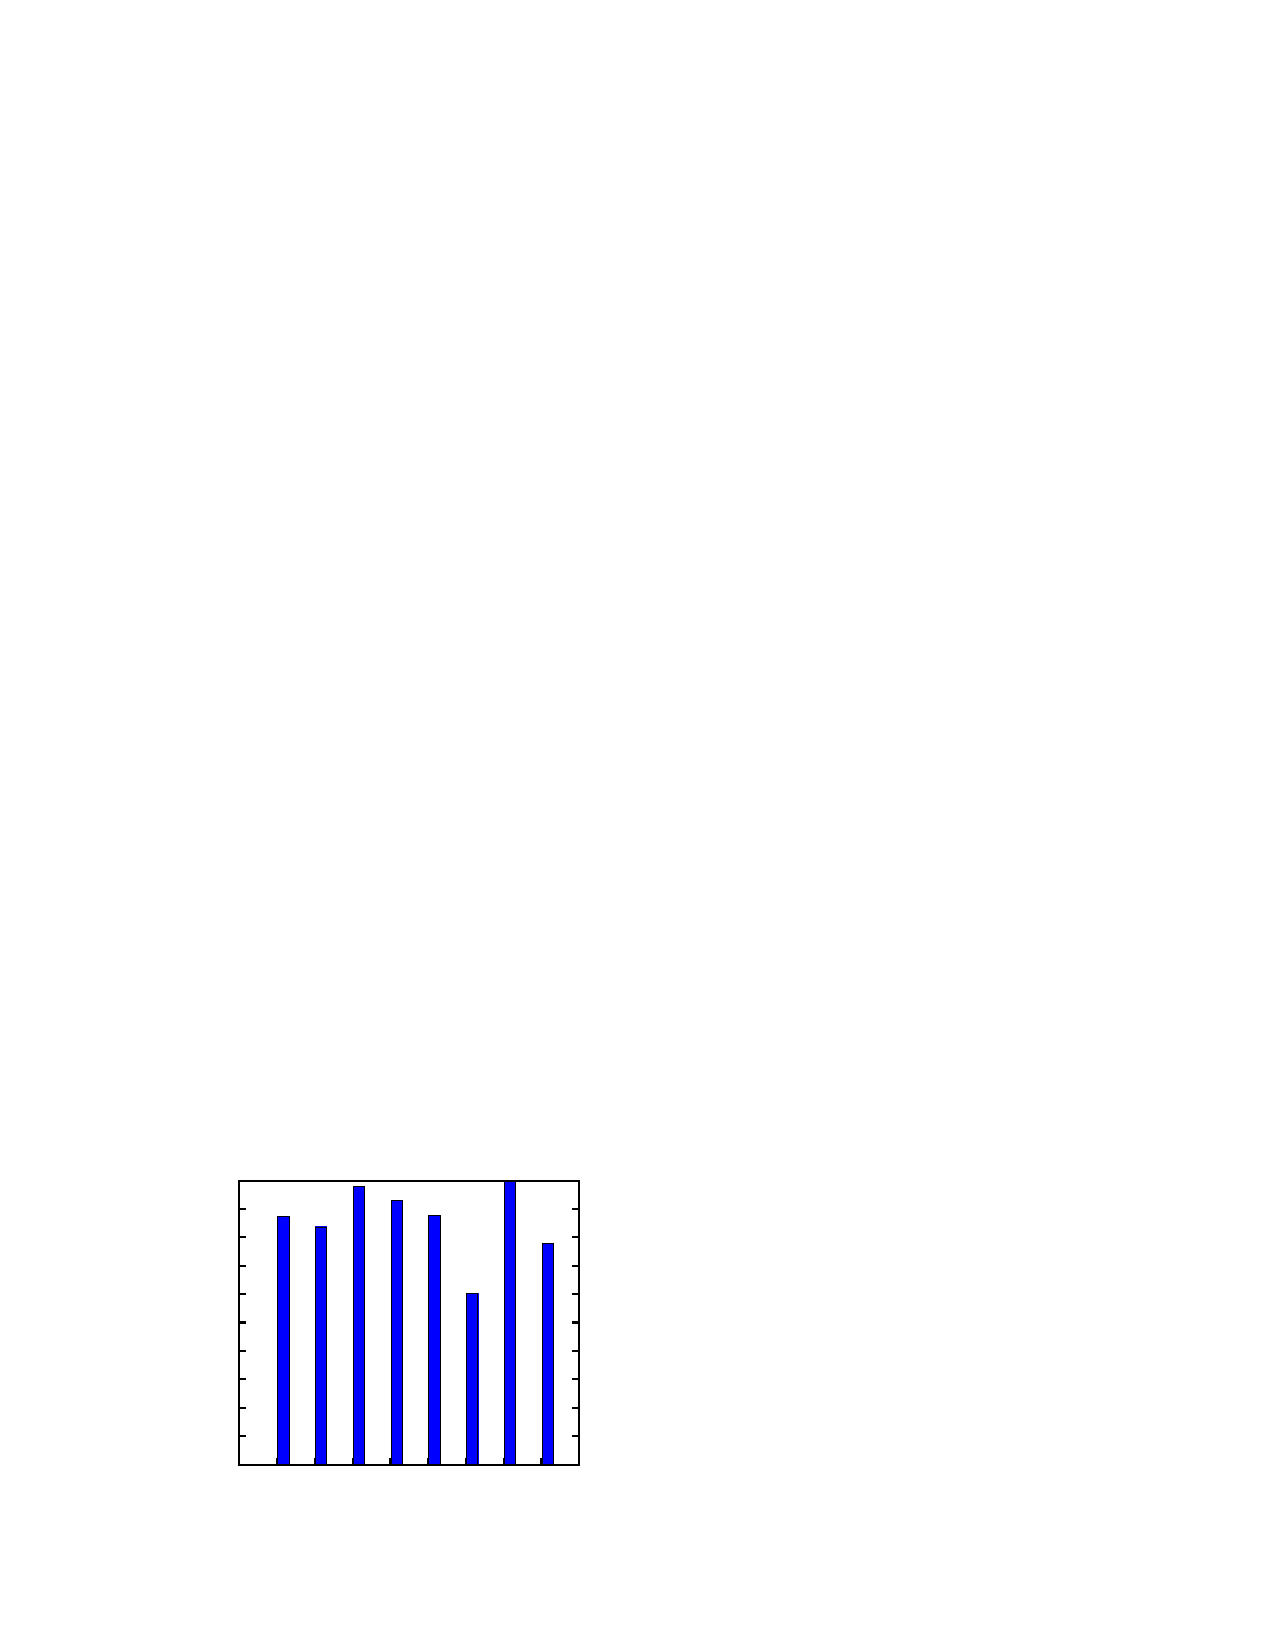
\includegraphics{img/nodes}}%
    \gplfronttext
  \end{picture}%
\endgroup

%\resizebox{\columnwidth}{2in}{% GNUPLOT: LaTeX picture with Postscript
\begingroup
  \makeatletter
  \providecommand\color[2][]{%
    \GenericError{(gnuplot) \space\space\space\@spaces}{%
      Package color not loaded in conjunction with
      terminal option `colourtext'%
    }{See the gnuplot documentation for explanation.%
    }{Either use 'blacktext' in gnuplot or load the package
      color.sty in LaTeX.}%
    \renewcommand\color[2][]{}%
  }%
  \providecommand\includegraphics[2][]{%
    \GenericError{(gnuplot) \space\space\space\@spaces}{%
      Package graphicx or graphics not loaded%
    }{See the gnuplot documentation for explanation.%
    }{The gnuplot epslatex terminal needs graphicx.sty or graphics.sty.}%
    \renewcommand\includegraphics[2][]{}%
  }%
  \providecommand\rotatebox[2]{#2}%
  \@ifundefined{ifGPcolor}{%
    \newif\ifGPcolor
    \GPcolortrue
  }{}%
  \@ifundefined{ifGPblacktext}{%
    \newif\ifGPblacktext
    \GPblacktextfalse
  }{}%
  % define a \g@addto@macro without @ in the name:
  \let\gplgaddtomacro\g@addto@macro
  % define empty templates for all commands taking text:
  \gdef\gplbacktext{}%
  \gdef\gplfronttext{}%
  \makeatother
  \ifGPblacktext
    % no textcolor at all
    \def\colorrgb#1{}%
    \def\colorgray#1{}%
  \else
    % gray or color?
    \ifGPcolor
      \def\colorrgb#1{\color[rgb]{#1}}%
      \def\colorgray#1{\color[gray]{#1}}%
      \expandafter\def\csname LTw\endcsname{\color{white}}%
      \expandafter\def\csname LTb\endcsname{\color{black}}%
      \expandafter\def\csname LTa\endcsname{\color{black}}%
      \expandafter\def\csname LT0\endcsname{\color[rgb]{1,0,0}}%
      \expandafter\def\csname LT1\endcsname{\color[rgb]{0,1,0}}%
      \expandafter\def\csname LT2\endcsname{\color[rgb]{0,0,1}}%
      \expandafter\def\csname LT3\endcsname{\color[rgb]{1,0,1}}%
      \expandafter\def\csname LT4\endcsname{\color[rgb]{0,1,1}}%
      \expandafter\def\csname LT5\endcsname{\color[rgb]{1,1,0}}%
      \expandafter\def\csname LT6\endcsname{\color[rgb]{0,0,0}}%
      \expandafter\def\csname LT7\endcsname{\color[rgb]{1,0.3,0}}%
      \expandafter\def\csname LT8\endcsname{\color[rgb]{0.5,0.5,0.5}}%
    \else
      % gray
      \def\colorrgb#1{\color{black}}%
      \def\colorgray#1{\color[gray]{#1}}%
      \expandafter\def\csname LTw\endcsname{\color{white}}%
      \expandafter\def\csname LTb\endcsname{\color{black}}%
      \expandafter\def\csname LTa\endcsname{\color{black}}%
      \expandafter\def\csname LT0\endcsname{\color{black}}%
      \expandafter\def\csname LT1\endcsname{\color{black}}%
      \expandafter\def\csname LT2\endcsname{\color{black}}%
      \expandafter\def\csname LT3\endcsname{\color{black}}%
      \expandafter\def\csname LT4\endcsname{\color{black}}%
      \expandafter\def\csname LT5\endcsname{\color{black}}%
      \expandafter\def\csname LT6\endcsname{\color{black}}%
      \expandafter\def\csname LT7\endcsname{\color{black}}%
      \expandafter\def\csname LT8\endcsname{\color{black}}%
    \fi
  \fi
  \setlength{\unitlength}{0.0500bp}%
  \begin{picture}(5040.00,3772.00)%
    \gplgaddtomacro\gplbacktext{%
      \csname LTb\endcsname%
      \put(1166,780){\makebox(0,0)[r]{\strut{} 0}}%
      \put(1166,1053){\makebox(0,0)[r]{\strut{} 0.1}}%
      \put(1166,1325){\makebox(0,0)[r]{\strut{} 0.2}}%
      \put(1166,1598){\makebox(0,0)[r]{\strut{} 0.3}}%
      \put(1166,1871){\makebox(0,0)[r]{\strut{} 0.4}}%
      \put(1166,2144){\makebox(0,0)[r]{\strut{} 0.5}}%
      \put(1166,2416){\makebox(0,0)[r]{\strut{} 0.6}}%
      \put(1166,2689){\makebox(0,0)[r]{\strut{} 0.7}}%
      \put(1166,2962){\makebox(0,0)[r]{\strut{} 0.8}}%
      \put(1166,3234){\makebox(0,0)[r]{\strut{} 0.9}}%
      \put(1166,3507){\makebox(0,0)[r]{\strut{} 1}}%
      \put(1661,648){\rotatebox{-45}{\makebox(0,0)[l]{\strut{}yearpredict}}}%
      \put(2023,648){\rotatebox{-45}{\makebox(0,0)[l]{\strut{}twitter}}}%
      \put(2386,648){\rotatebox{-45}{\makebox(0,0)[l]{\strut{}tinyImages}}}%
      \put(2748,648){\rotatebox{-45}{\makebox(0,0)[l]{\strut{}mnist}}}%
      \put(3111,648){\rotatebox{-45}{\makebox(0,0)[l]{\strut{}corel}}}%
      \put(3473,648){\rotatebox{-45}{\makebox(0,0)[l]{\strut{}covtype}}}%
      \put(3836,648){\rotatebox{-45}{\makebox(0,0)[l]{\strut{}artificial40}}}%
      \put(4198,648){\rotatebox{-45}{\makebox(0,0)[l]{\strut{}faces}}}%
      \put(176,2143){\rotatebox{-270}{\makebox(0,0){\strut{}fraction of nodes in the original cover tree }}}%
      \put(396,2143){\rotatebox{-270}{\makebox(0,0){\strut{} required for the simplified cover tree}}}%
    }%
    \gplgaddtomacro\gplfronttext{%
    }%
    \gplbacktext
    \put(0,0){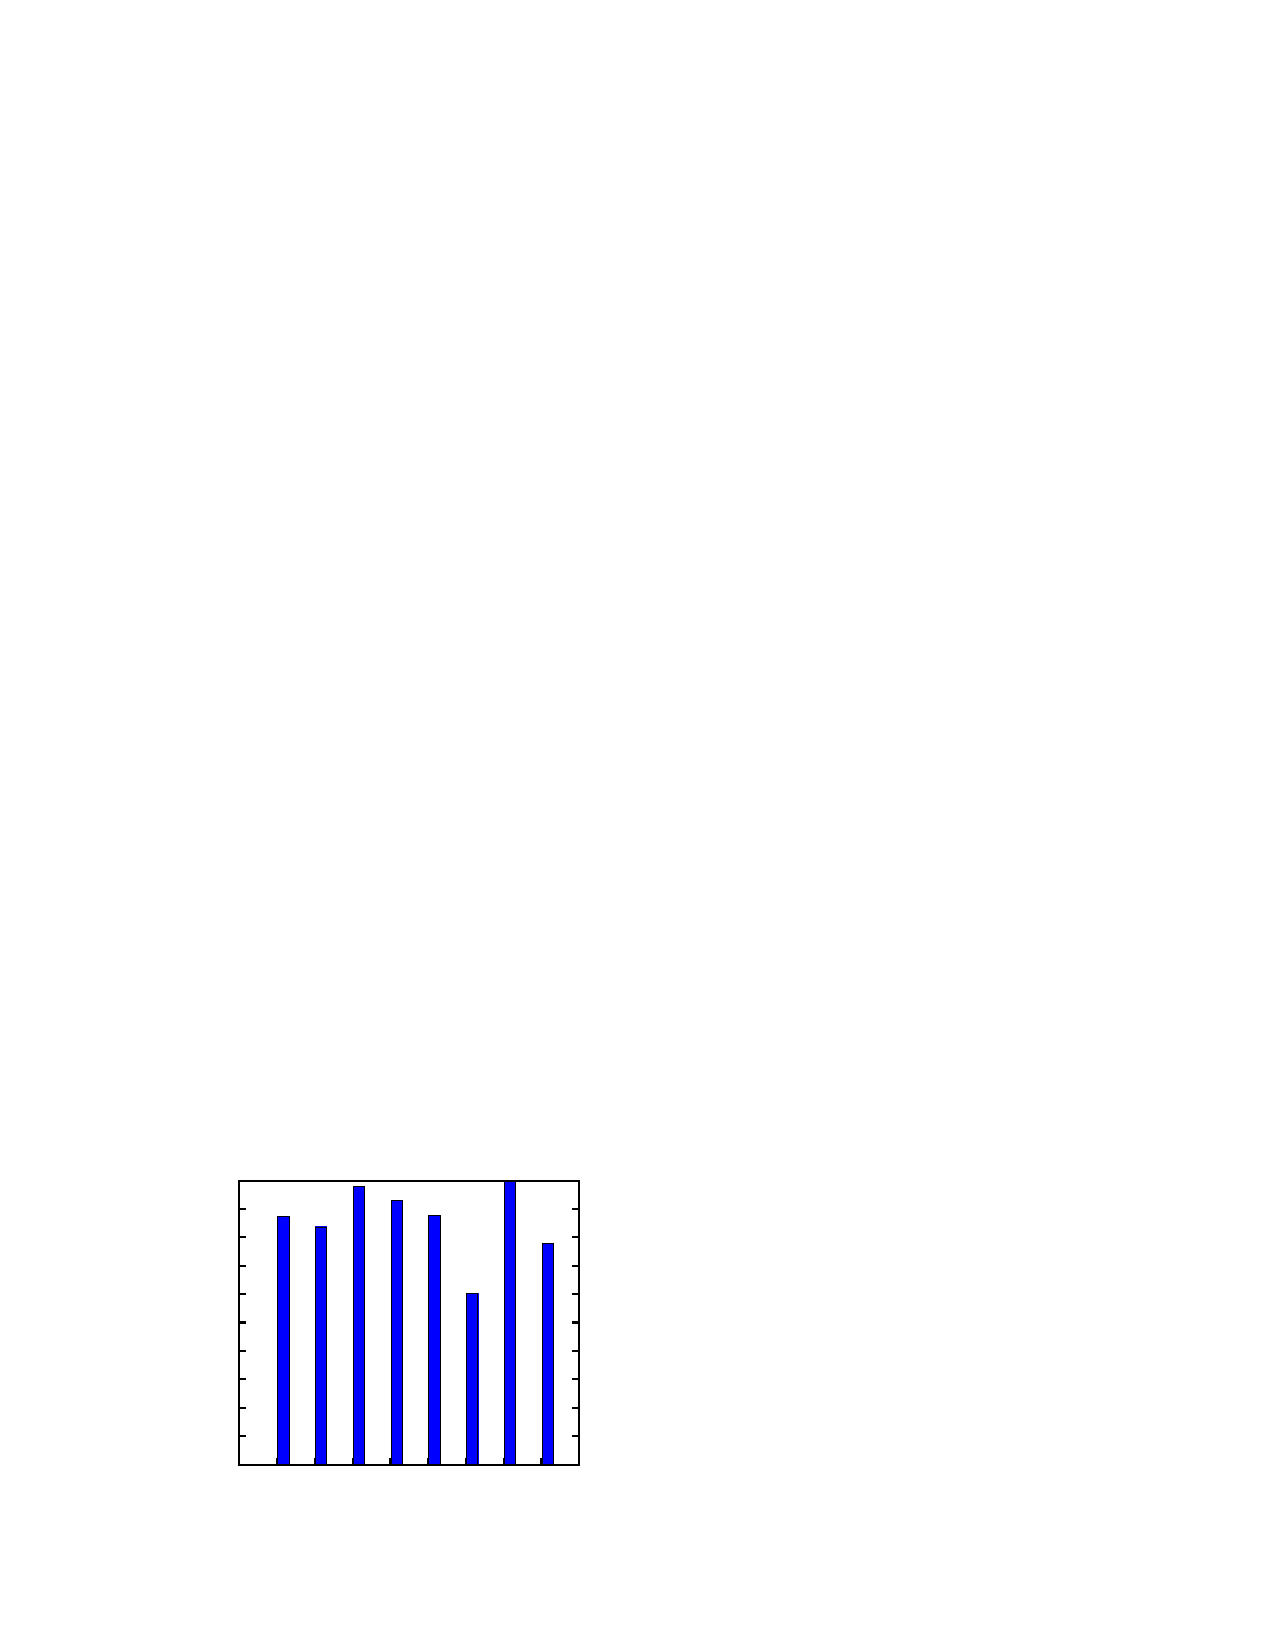
\includegraphics{img/nodes}}%
    \gplfronttext
  \end{picture}%
\endgroup
}
%\resizebox{\columnwidth}{2in}{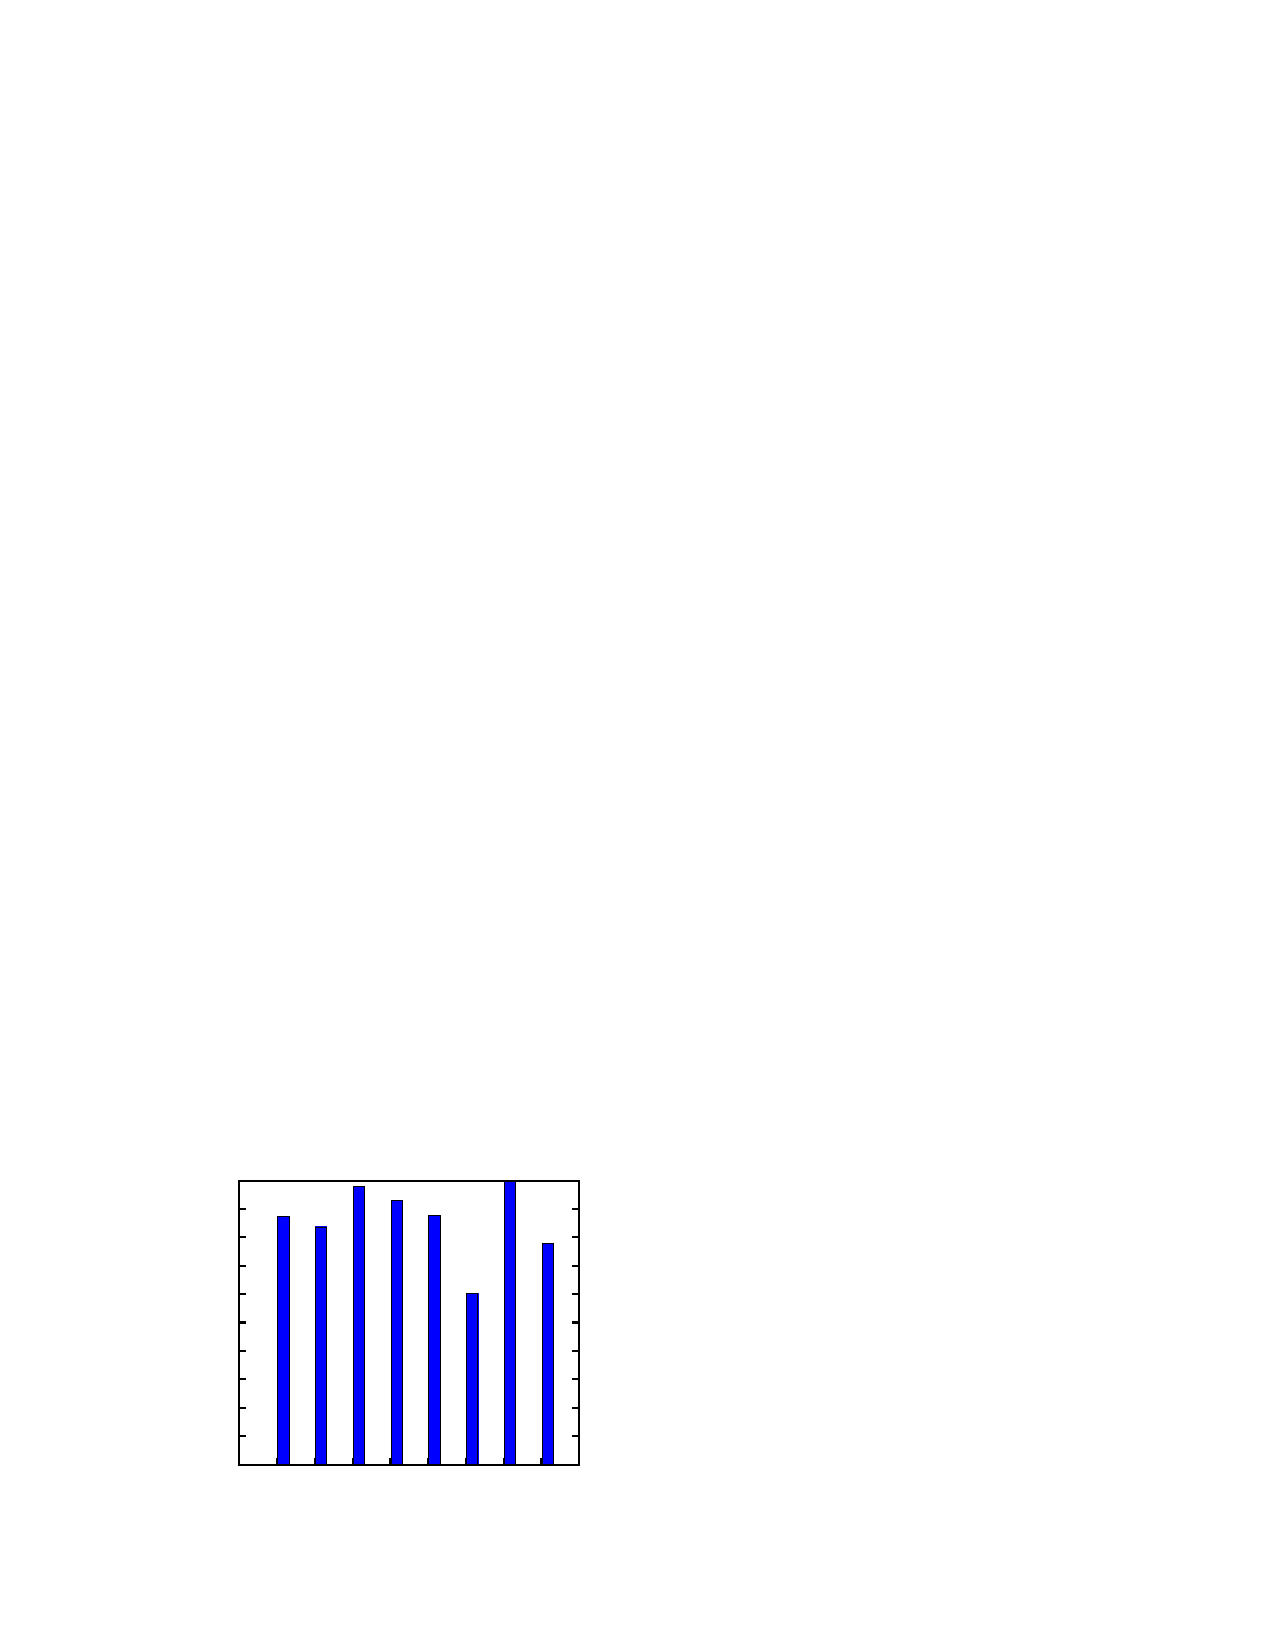
\includegraphics{./img/nodes}}
%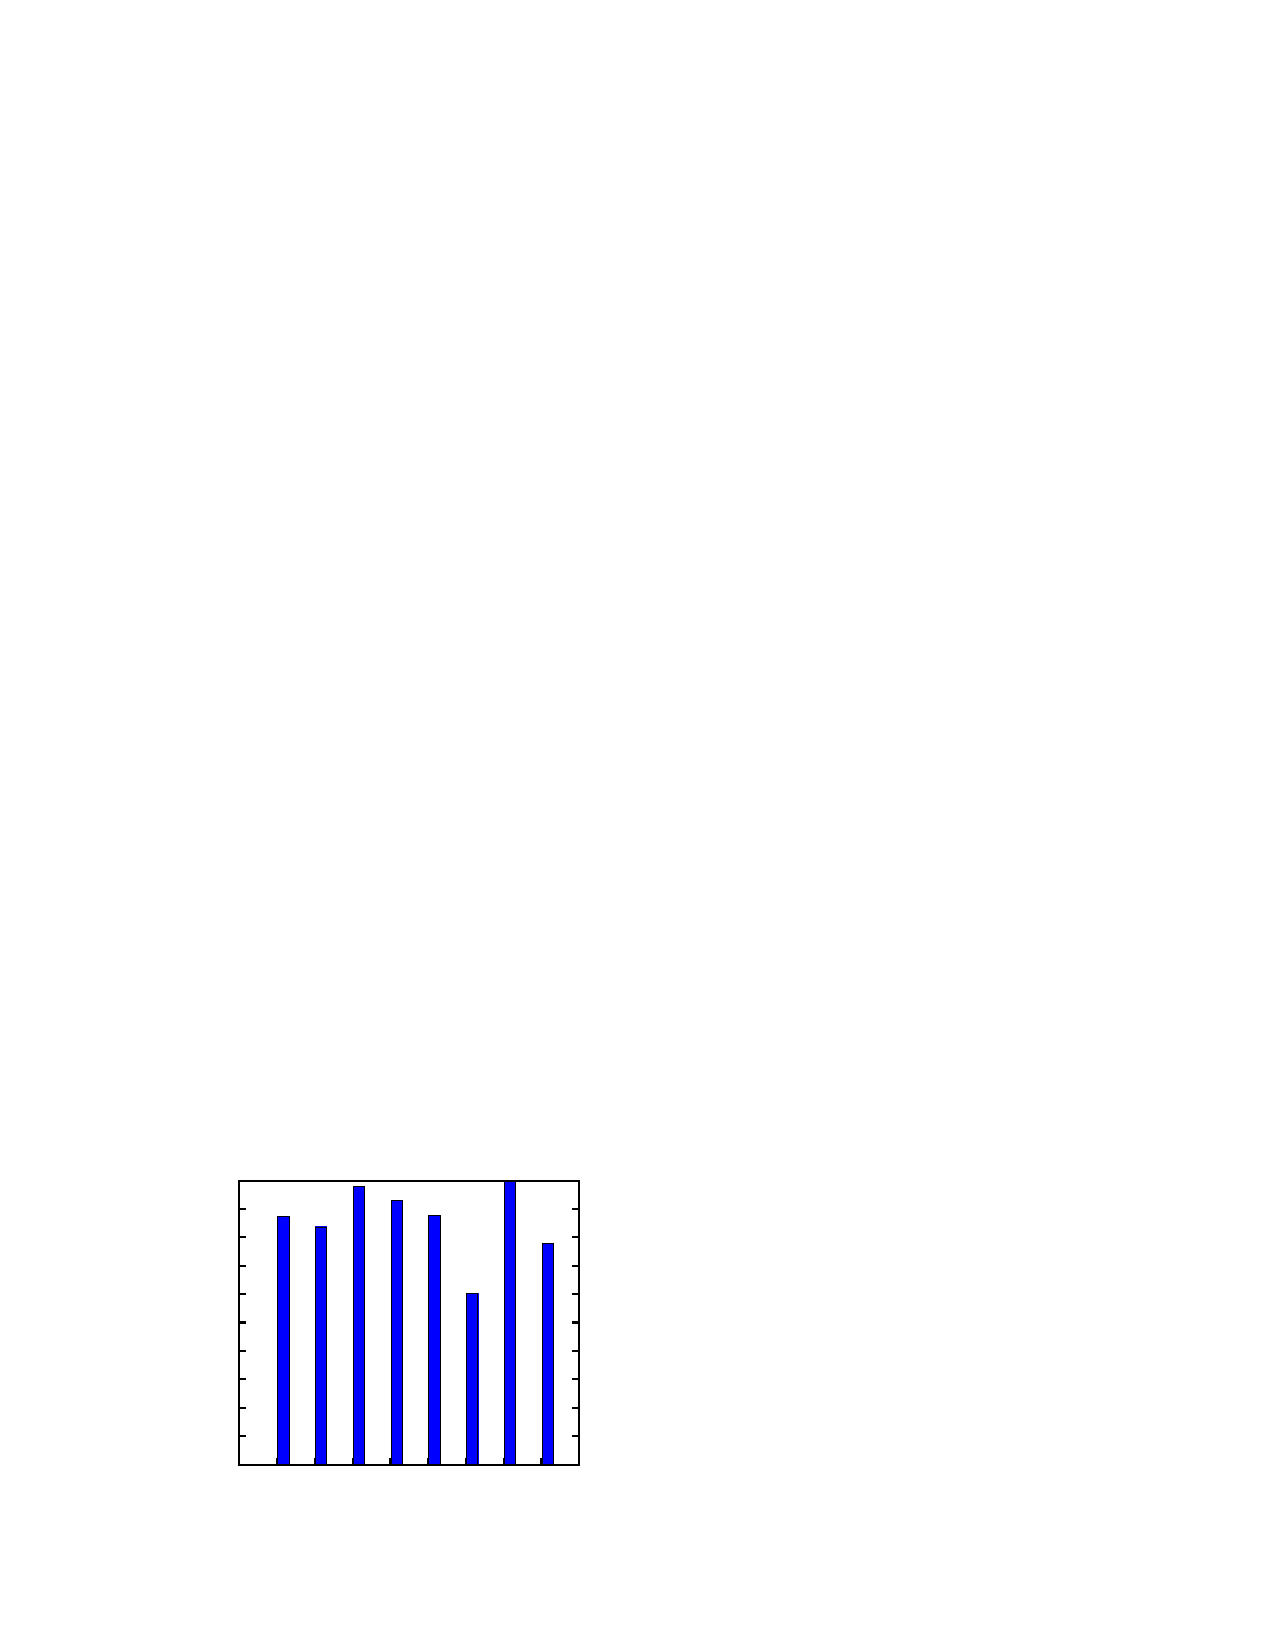
\includegraphics[width=9cm,height=6cm]{img/nodes}
\caption{
	Fraction of nodes required for the simplified cover tree.
    Fewer nodes means less overhead from traversing the tree and fewer distance comparisons.
    See Table \ref{tab:datasets} for information on the datasets.
    }
\label{fig:nodes}
\end{figure}

%%%%%%%%%%%%%%%%%%%%%%%%%%%%%%%%%%%%%%%%

%\subsection{Approximate nearest neighbor queries}
%\begin{algorithm}[t]
    %\caption{ \findnn(cover tree $p$, query  point $x$, nearest neighbor so far $y$)}
    %\label{alg:query}
%
    %\vspace{0.1in}
%\begin{algorithmic}[1]
    %\If {$d(p,x) < d(y,x)$}
        %\State $y \leftarrow p$
    %\EndIf
    %\For {each child $q$ of $p$ sorted by distance to $x$}
        %\If {$d(y,x) > d(y,q) - \maxdist{q}$} %2^{\level q}$}
            %\State $y \leftarrow \findnn(q,x,y)$
        %\EndIf
    %\EndFor
    %\State\Return $y$
%\end{algorithmic}
%\end{algorithm}

%%%%%%%%%%%%%%%%%%%%%%%%%%%%%%%%%%%%%%%%

\subsection{Inserting a single point}

\begin{algorithm}[t]
%\caption{Simplified cover tree insertion}
    \caption{\ctinsert(cover tree $p$, data point $x$)}
\label{alg:insert}

\begin{algorithmic}[1]
    \If {$\dist p x > \covdist p$}
        \While {$\dist p x > 2\covdist p$}
            \State Remove any leaf $q$ from $p$
            \State $p' \leftarrow $ tree with root $q$ and $p$ as only child
		  \State $p \leftarrow p'$
        \EndWhile
        \State\Return tree with $x$ as root and $p$ as only child
    \EndIf
    \State\Return \ctinsertHelper($p$,$x$)
\end{algorithmic}
\end{algorithm}

\begin{algorithm}[t]
    \caption{\ctinsertHelper(cover tree $p$, data point $x$)}
    \label{alg:insertloop}
    \vspace{0.1in}
prerequisite: $\dist p x \le \covdist p$

\begin{algorithmic}[1]
    \For {$q \in \children{p}$}
        \If {$\dist q x \le \covdist q$}
            \State $q' \leftarrow \ctinsertHelper(q,x)$
            \State $p' \leftarrow p$ with child $q$ replaced with $q'$
            \State \Return $p'$
        \EndIf
    \EndFor
    \State\Return $p$ with $x$ added as a child
\end{algorithmic}
\end{algorithm}

Insertion into a simplified cover tree is faster and simpler than the original cover tree.
Algorithms \ref{alg:insert} and \ref{alg:insertloop} show the procedure.
It is divided into two cases.
In the first case, we cannot insert our data point $x$ into the tree without violating the covering invariant.
So we raise the level of the tree $p$ by taking any leaf node and using that as the new root.
Because $\maxdist{p} \le 2\covdist{p}$, we are guaranteed that $d(p,x) \le \covdist{x}$, and so we do not violate the covering constraint.
In the second case, the \ctinsertHelper~function recursively descends the tree.
On each function call, we search through $\children{p}$ to find a node we can insert into without violating the covering invariant.
If we find such a node, we recurse; otherwise, we know we can add $x$ to $\children{p}$ without violating the separating invariant.
In all cases, exactly one node is added per data point, so the resulting tree will have exactly $n$ nodes.
The following theorem shows that inserting into a simplified cover tree has a better dependence on $\cdoub$ than inserting into the original cover tree ($\cdoub^2$ vs $\cdoub^3$).

\begin{theorem}
    The runtime of $\ctinsertHelper(p,x)$ is $O(\cdoub^2\log \aspect{})$.
    For i.i.d.\ data satisfying the regularity conditions of Lemma \ref{lemma:Easpect},
    the expected runtime is $O(\cdoub^2\log n)$.
\end{theorem}
\begin{proof}
    On each recursive call,
    the algorithm visits each child node at most once,
    then either descends a level or terminates.
    The number of children is bounded by $O(\cdoub^2)$ by Lemma \ref{lemma:children},
    and the height of the tree is bounded by $O(\log \aspect{})$ by Lemma \ref{lemma:height}.
    In the i.i.d.\ case, Lemma \ref{lemma:Easpect} states that $\aspect{} = O(n^3)$.
\end{proof}

%%%%%%%%%%%%%%%%%%%%%%%%%%%%%%%%%%%%%%%%

\subsection{The nearest ancestor invariant}

A further advantage of the simplified cover tree is that it is easier to add new invariants that improve performance.
In this section, we exploit a similarity between simplified cover trees and binary search trees (BSTs).
Insertion into both trees follows the same procedure:
Perform a depth first search to find the right location to insert the point.
In particular, there is no rebalancing after the insertion.
Many alternatives to plain BSTs produce better query times by introducing new invariants.
These invariants force the insertion algorithm to rebalance the tree during the insertion step.
% cshelton1: is the following statement correct?  Insertion into an AVL tree is faster than into a BST
% (at least if we hold the elements in the tree fixed, and not the exact tree) because the depth of
% the tree is smaller.
% mike: I think it depends on exactly what you mean by "faster".
% On any particular tree, doing a BST insertion will be faster because there's no need to rebalance; but doing a series of AVL insertion may be faster if it avoids worst case BST behavior.
% I think in the cover tree case, the rebalancing step is expensive enough compared to the gains from balancing that you almost always end up slower.
Our definition of the simplified cover tree makes adding similar invariants easy.
%This gives us faster query times in exchange for a longer tree construction.
We now introduce one possible invariant.

%\begin{defn}
A \emph{nearest ancestor cover tree} is a simplified cover tree where every point $p$ has the nearest ancestor invariant:
If $q_1$ is an ancestor of $p$ and $q_2$ is a sibling of $q_1$, then
$$
d(p,q_1) \le d(p,q_2)
$$
%\end{defn}
In other words, the nearest ancestor cover tree ensures that for every data point, each of its ancestors is the ``best possible'' ancestor for it at that level.%
\footnote{
The nearest ancestor invariant is incompatible with the global separating invariant of the original cover tree.
There are data sets that cannot simultaneously satisfy both.
}
Figure \ref{fig:nearestancestorexample} shows a motivating one dimensional example.

\begin{figure}
\definecolor{lightred}{rgb}{1,0.8,0.8}
\definecolor{lightgreen}{rgb}{0.8,1,0.8}
\centering
\begin{tikzpicture}
    [ draw
    , scale=1.8
    , every node/.style={minimum size=9mm,fill=white}
    , level/.style={sibling distance = 18mm/#1, level distance=12mm}
    %,    level distance = 1.5cm}
    , sibling distance=8mm
    ]
\draw (-2,0) -- (6.3,0)[dotted];
\draw (-2,-12mm) -- (6.3,-12mm)[dotted];
\draw (-2,-24mm) -- (6.3,-24mm)[dotted];
\node[shape=circle,draw] at (0,0) {10}
    child { node[circle,draw] {8}
        child { node[circle,draw] {7}  }
        child { node[circle,draw,fill=lightred,line width=1pt] {11} }
        }
    child { node[circle,draw] {12}
        child { node[circle,draw,fill=lightred,line width=1pt] {9}  }
        child { node[circle,draw] {13} }
        }
    ;
\node[shape=circle,draw] at (3.5,0) {10}
    child { node[circle,draw] {8}
        child { node[circle,draw] {7}  }
        child { node[circle,draw,fill=lightgreen,line width=1pt] {9} }
        }
    child { node[circle,draw] {12}
        child { node[circle,draw,fill=lightgreen,line width=1pt] {11}  }
        child { node[circle,draw] {13} }
        }
    ;
\node[fill=none] at (5.8,3mm) {level 3};
\node[fill=none] at (5.8,-9mm) {level 2};
\node[fill=none] at (5.8,-21mm) {level 1};
\end{tikzpicture}
\caption{
    Using the metric $d(a,b)=|a-b|$,
    both trees are valid simplified cover trees;
    but only the right tree is a valid nearest ancestor cover tree.
    %Moving the 9 and 11 nodes reduces the value of $\mkfunction{maxdist}$ for their ancestor nodes.
    Moving the 9 and 11 nodes reduces the value of maxdist for their ancestor nodes.
    This causes pruning to happen more often during nearest neighbor queries (Algorithm \ref{alg:query}), resulting in fewer distance comparisons.
    }
\label{fig:nearestancestorexample}
\end{figure}

Algorithm \ref{alg:nearestancestor} shows how to insert a point into a nearest ancestor cover tree.
It uses the same \ctinsert~function as \ref{alg:insert}, but the helper function \ctinsertHelper~is slightly modified in two ways (shown with an \underline{underline}).
First, we sort $\children{p}$ according to their distance from the data point $x$.
This sorting ensures that our newly inserted point will satisfy the nearest ancestor invariant.
But this new point $x$ may cause other points to violate the nearest ancestor invariant.
In particular, if $x$ has a sibling $q$; $q$ has a descendent $r$; and $\dist r x < \dist r q$; then $r$ now violates the nearest ancestor invariant.
Our second step is to call $\mkfunction{rebalance}$, which finds all these violating data points and moves them underneath $x$.
%Edge cases make rebalancing look awkward.
%Rebalancing is awkward only because there are many edge cases to check.

Most of the work of the $\rebalance$ function happens in the helper $\rebalanceHelper$.
$\rebalanceHelper$ returns a valid nearest ancestor cover tree and a set of points that still need to be inserted;
$\rebalance$ just inserts those extra points.
$\rebalanceHelper$ takes two nearest ancestor cover trees $p$ and $q$ (where $p$ is an ancestor of $q$) and a point $x$.
Its goal is to ``extract'' all points from $q$ that would violate the nearest ancestor invariant if $x$ became a sibling of $p$.
It returns three values:
a modified version of $q$,
a set of points that cannot remain in any point along the path from $p$ to $q$ called the \mkvar{moveset},
and a set of points that need to be reinserted somewhere along the path from $p$ to $q$ called the \mkvar{stayset}.
There are two cases.
In the first case, the data point at node $q$ must move.
We then filter the descendants of $q$ into the \mkvar{moveset} or \mkvar{stayset} as appropriate and return \nullvar\ for our modified $q$.
In the second case, the data point at node $q$ must stay.
We recursively apply \rebalanceHelper~to each of $q$'s children;
we use the results to update the corresponding child, the \mkvar{moveset} and the \mkvar{stayset} variables.
Finally, we try to reinsert any nodes in \mkvar{stayset}.
If \rebalanceHelper~was called with $q$ a child of $p$, then the return value of \mkvar{stayset} will be empty;
any children that could not be directly reinserted must be in the \mkvar{moveset}.

%\textcolor{red}{
The \rebalanceHelper~function loops over all $O(\cdoub^2)$ children of a node, and the maximum depth of the recursion is $O(\log \aspect{})$.
Therefore the overall runtime is $O(\cdoub^2 \log \aspect{})$.
% cshelton1: check the line reference below
It may be called up to $O(\cdoub^2)$ times within \rebalance, 
so the body of the for loop on line~\ref{rebalanceloop} executes $O(\cdoub^4\log\aspect{})$ times.
Unfortunately, we have no bound on the size of \emph{moveset}, except to note that it is usually small in practice.
On the datasets in our experiments (see Table \ref{tab:datasets}), the value is usually zero or at worst in the single digits.
%This is a rather unsatisfying theoretical analysis, but empirical performance is good.
%}
Figure \ref{fig:numdist}(a) shows that nearest ancestor cover tree construction is not that much slower in practice,
and Figure \ref{fig:numdist}(b) shows that this slowdown is overshadowed by the resulting speedup in nearest neighbor queries.

\begin{algorithm}[t!]
    %\caption{Nearest ancestor cover tree insertion}
    \caption{\ctinsertHelper(cover tree $p$, data point $x$)}
    \label{alg:nearestancestor}

    \vspace{0.1in}

\begin{algorithmic}[1]
    \For {$q \in \children{p}$ \underline{sorted by distance to $x$}}
        \If {$\dist q x \le \covdist q$}
            \State $q' \leftarrow \ctinsertHelper(q,x)$
            \State $p' \leftarrow p$ with child $q$ replaced with $q'$
            \State \Return $p'$
        \EndIf
    \EndFor
    \State \Return \underline{\mkprocedure{rebalance}($p$, $x$)}
\end{algorithmic}
\end{algorithm}

\begin{algorithm}[t]
{\bfseries function} \mkprocedure{rebalance}(cover trees $p$, data point $x$)

\emph{prerequisites:} $x$ can be added as a child of $p$ without violating the covering or separating invariants

\begin{algorithmic}[1]
    %\State $x' \leftarrow $ tree with root $x$ and level $\level{p}-1$
    \State create tree $x'$ with root node $x$ at level $\level{p}-1$
           $x'$ contains no other points
    \State $p' \leftarrow p$
    \For { $q \in \children{p}$}
        \State $(q',moveset,stayset) \leftarrow \rebalanceHelper(p,q,x)$
        \State $p' \leftarrow p'$ with child $q$ replaced with $q'$
        \For {$r \in moveset$}
            \State $x' \leftarrow \ctinsert(x',r)$
        \EndFor
    \EndFor
    \State\Return $p'$ with $x'$ added as a child
\end{algorithmic}
\end{algorithm}

\begin{algorithm}[t]
    \caption{\rebalanceHelper(cover trees $p$ and $q$, point $x$)}

    \vspace{0.1in}
    \vspace{0.1in}
\emph{prerequisites:} $p$ is an ancestor of $q$

\begin{algorithmic}[1]
    \If {$\dist p q > \dist q x$}
        \State $moveset, stayset \leftarrow \emptyset$
        \For {$r \in \descendants q$}
            \If {$\dist r p > \dist r x$}
                \State $moveset \leftarrow moveset \cup \{r\}$
            \Else
                \State $stayset \leftarrow stayset \cup \{r\}$
            \EndIf
        \EndFor
        \State\Return $(\nullvar, moveset, stayset)$
        %\State\Return (\nullvar, $\{q\} \cup $descendants closer to q, descendants closer to x)
    \Else
        \State $\mkvar{moveset}',\mkvar{stayset}' \leftarrow \emptyset$
        \State $q' \leftarrow q$
        %\State $\mkvar{moveset}',\mkvar{stayset}' \leftarrow \emptyset$
        %\State $q' \leftarrow q$
        \For {$r \in \children q$} \label{rebalanceloop}
            \State $(r',moveset,stayset) \!\leftarrow\! \rebalanceHelper(p,r,x)$
            \State $\mkvar{moveset}' \leftarrow \mkvar{moveset}\cup\mkvar{moveset}'$
            \State $\mkvar{stayset}' \leftarrow \mkvar{stayset}\cup\mkvar{stayset}'$
            \If {$r' = \nullvar$}
                \State $q' \leftarrow q$ with the subtree $r$ removed
            \Else
                \State $q' \leftarrow q$ with the subtree $r$ replaced by $r'$
                %\State $r'' \leftarrow $ insert stayset into $r'$
            \EndIf
        \EndFor
        \For {$r \in stayset'$}
            \If {$\dist r q' \le \covdist q'$}
                \State $q' \leftarrow \ctinsert (q',r)$
                \State $\mkvar{stayset}' \leftarrow \mkvar{stayset}' - \{r\}$
            \EndIf
        \EndFor
        \State\Return $(q',moveset',stayset')$
    \EndIf
\end{algorithmic}
\end{algorithm}

%%%%%%%%%%%%%%%%%%%%%%%%%%%%%%%%%%%%%%%%

\subsection{Merging simplified cover trees}

In this section we discuss parallelism on shared-memory, multiprocessor machines.
Querying in parallel is easy.
%Querying a cover tree in parallel is easy.
Since the results of neighbor queries for a data point do not depend on other data points, we can:
divide the points among the processors;
then each processor traverses the tree independently.
More difficult is constructing the tree in parallel.
Our strategy is to split the data, create one cover tree on each processor, then merge these trees together.
Previous work on parallelizing cover trees applied only to the GPU \citep{Kumar2010}.
Our approach is suitable for any shared-memory multiprocessor machine.
We give a detailed description for merging simplified cover trees and discuss at a high level how to extend this procedure to nearest ancestor cover trees.

Algorithm \ref{alg:merge} shows the merging procedure.
The \mkprocedure{merge} function's main purpose is to satisfy the prerequisites for \mkprocedure{mergeHelper}, which has two phases.
%Most of this work is done in the \mkprocedure{mergeHelper} function.
%\mkprocedure{mergeHelper} has two phases.
First, we find all the subtrees of $q$ that can be inserted directly into $p$ without violating any invariants, and we insert them.
Second, we insert the remaining nodes from $q$ into $p$ directly via the \ctinsert~function.

The \mkprocedure{mergeHelper} function returns a partially merged tree and a set of nodes called the \mkvar{leftovers} that still need to be inserted into the tree.
The first phase uses the for loop starting on line~\ref{mergeloop} to categorize the children of $q$ into three disjoint sets.
The \mkvar{uncovered} set contains all of $q$'s children that would violate the covering invariant if inserted into $p$.
The \mkvar{sepcov} set contains all of $q$'s children that would not violate the separating or covering invariants when inserted into $p$.
Both of these sets are unused in the second phase of \mkprocedure{mergeHelper}.
Every child of $q$ that is not inserted into the \mkvar{uncovered} or \mkvar{sepcov} sets gets merged with a suitable node in $\children{p}$.
This is done by recursively calling the \mkprocedure{mergeHelper} function.
Any points that could not be inserted into the results of \mkprocedure{mergeHelper} get added to the \mkvar{leftovers} set.

In the second phase of \mkprocedure{mergeHelper}, we insert as many nodes as possible into our merged tree $p'$.
First update the children with the subtrees in \mkvar{sepcov}.
Then insert the root of $q$.
We know that $d(p,q) \le \covdist{p}$, so this insertion is guaranteed not to change the level of $p'$.
Finally, we loop over the elements in \mkvar{leftovers} and insert them into $p'$ only if it would not change the level of $p'$.
Any elements of \mkvar{leftovers} that cannot be inserted into $p'$ get inserted into $\mkvar{leftovers}'$ and returned.
It is important to do this insertion of \mkvar{leftovers} at the lowest level possible (rather than wait until the recursion ends and have the insertion performed in \mkprocedure{merge}) to avoid unnecessary distance computations.

%Extending \mkprocedure{merge} to work on nearest ancestor cover trees requires a similar procedure to how we modified \ctinsert.
%Extending \mkprocedure{merge} to work on nearest ancestor cover trees requires the following rebalancing operations.
The \mkprocedure{merge} function does not maintain the nearest ancestor invariant.
A modified version of \mkprocedure{merge} that calls the \rebalance~function appropriately could.
But for space reasons, we do not provide this modified algorithm.
In our experiments below, we use the provided \mkprocedure{merge} function in Algorithm \ref{alg:merge} to parallelize both simplified and nearest ancestor tree construction.
In practice, this retains the benefits of the nearest ancestor cover tree because the nearest ancestor invariant is violated in only a few places.

Providing explicit bounds on the runtime of \mkprocedure{merge} is difficult.
%We cannot give any bounds on the runtime of \mkprocedure{merge}.
But in practice it is fast.
When parallelizing on two processors, approximately 1\% of the distance calculations occur within \mkprocedure{merge}. %the merge operation typically requires about 1\% of the total distance comparisons.
So this is not our bottleneck.
Instead, the main bottleneck of parallelism is cache performance.
On modern desktop computers, last level cache is shared between all cores on a CPU.
Cover tree construction results in many cache misses,
and this effect is exaggerated when the tree is constructed in parallel.
%The next section improves cache performance, and the following section provides experimental results on parallel speedup.

%The next section discusses how to improve cache performance, and the following section provides experimental results on parallel speedup.
%The next section provides guidance on better cache performance on the CPU, and the following section provides experimental results on parallel speedup.
%\fixme{I'm pretty sure this algorithm should be $o(c^{O(1)}n)$ (the little o is correct), but I can't think of a proof.}

\begin{algorithm}[t!]
%\caption{Merging cover trees}
    \caption{ \mkprocedure{merge}(cover tree $p$, cover tree $q$)}
\label{alg:merge}

\vspace{0.1in}

\begin{algorithmic}[1]
\If {$\level q > \level p$}
	\State swap $p$ and $q$
    %\State $p' \leftarrow q$; $q' \leftarrow p$
%\Else
%    \State $p' \leftarrow p$; $q' \leftarrow q$
\EndIf

\While {$\level q < \level p$}
    \State move a node from the leaf of $q$ to the root;
    \State this raises the level of $q$ by 1
\EndWhile

\State $(p,leftovers) \leftarrow \mkprocedure{mergeHelper}(p,q)$
\For {$r \in leftovers$}
    \State $p \leftarrow \ctinsert(p,r)$
\EndFor
\State\Return $p$

\end{algorithmic}
\end{algorithm}
\begin{algorithm}
    \caption{ \mkprocedure{mergeHelper}(cover tree $p$, cover tree $q$)}

%\emph{prerequisite:} $\level{p}=\level{q}$

%\emph{prerequisite:} $d(p,q) \le \covdist p$
    \vspace{0.1in}
\emph{prerequisite:} $\level{p}=\level{q}$, $d(p,q)\le\covdist p$


\begin{algorithmic}[1]
\State $\mkvar{children}' \leftarrow \children p$ \Comment{Phase 1}
\State $\mkvar{uncovered}, \mkvar{sepcov}, \mkvar{leftovers} \leftarrow \emptyset$
\For { $r \in \children q $} \label{mergeloop}
    \If {$\dist p r < \covdist p$}
            \State $\mkvar{foundmatch} \leftarrow $\FALSE
            \For {$s \in \mkvar{children}'$}
                \If {$\dist s r \le \sepdist p$}
                    \State $(s',\mkvar{leftovers}_s) \leftarrow \mkprocedure{mergeHelper}(s, r)$
                    \State $\mkvar{children}' \leftarrow \mkvar{children}' \cup \{s'\} - \{s\}$
                    \State $\mkvar{leftovers} \leftarrow \mkvar{leftovers} \cup \mkvar{leftovers}_s$
                    \State $\mkvar{foundmatch} \leftarrow \TRUE$
                    \State {\bfseries break} from inner loop
                \EndIf
            \EndFor
            \If {\NOT $\mkvar{foundmatch}$}
                \State $\mkvar{sepcov} \leftarrow\mkvar{sepcov} \cup \{r\}$
            \EndIf
    \Else
        \State $\mkvar{uncovered} \leftarrow\mkvar{uncovered} \cup \{r\}$
    \EndIf
\EndFor

%\State $children',sepcov,leftovers \leftarrow \emptyset$
\State $\mkvar{children}' \leftarrow \mkvar{children}' \cup \mkvar{sepcov}$ \Comment{Phase 2}
\State $p' \leftarrow $ tree rooted at $p$ with $\children{p'}=\mkvar{children}'$
%\State $\children{p} \leftarrow \children{p} \cup \mkvar{sepcov}$
\State $p' \leftarrow \ctinsert(p',q)$
\State $\mkvar{leftovers}' \leftarrow \emptyset$
\For {$r \in \mkvar{leftovers}$}
    \If {$\dist r p' \le \covdist p'$}
        \State $p' \leftarrow \ctinsert(p',r)$
    \Else
        \State $\mkvar{leftovers}' \leftarrow \mkvar{leftovers}' \cup \{r\}$
    \EndIf
\EndFor
\State\Return $(p',\mkvar{leftovers}' \cup \mkvar{uncovered})$
\end{algorithmic}
\end{algorithm}

%%%%%%%%%%%%%%%%%%%%%%%%%%%%%%%%%%%%%%%%

\subsection{Cache efficiency}
\label{sec:cache}

One of the biggest sources of overhead in modern data structures is cache misses.
Our last improvement is to make cover trees more cache efficient.
A simple way to reduce cache misses for tree data structures is to use the \emph{van Emde Boas} tree layout
\cite{frigo1999}.
This layout arranges nodes in memory according to a depth first traversal of the tree.
This arrangement creates a \emph{cache oblivious} data structure.
That is, the programmer does not need any special knowledge about the cache sizes to obtain optimal speedup---the van Embde Boas tree layout works efficiently on any cache architecture.
This layout has been known for a long time in the data structures community, but it seems unused in machine learning libraries.
\citet{frigo1999} provides a detailed tutorial.

Our implementation of the cache oblivious cover tree is \emph{static}.
That is, we first construct the cover tree, then we call a function \pack~that rearranges the tree in memory.
This means we do not get the reduced cache misses while constructing the tree, but only while querying the tree.
The \pack\ function is essentially free to run because it requires only a single traversal through the dataset and no distance computations.
Figure \ref{fig:cache} shows that the van Emde Boas tree layout reduces cache misses by 5 to 20 percent.
This results in a reduction of stalled CPU cycles by 2 to 15 percent.

%%%%%%%%%%%%%%%%%%%%%%%%%%%%%%%%%%%%%%%%%%%%%%%%%%%%%%%%%%%%%%%%%%%%%%%%%%%%%%%%

\section{Experiments}
\label{sec:experiments}

%In this section we validate our improvements empirically.
We now validate our improvements to the cover tree empirically.
Our first experiments use the Euclidean distance on a standard benchmark suite (described in Table \ref{tab:datasets}).
%First, we use a standard benchmark suite described in Table \ref{tab:datasets} and the Euclidean distance.
%We compare the number of distance comparisons used by the three cover tree variants, and we compare our cover tree implementation to previous implementations of the original cover tree.
Our last experiments use non-Euclidean metrics on data from bioinformatics and computer vision.
In each experiment, we use the \defn{all nearest neighbors} experimental setup.
That is, we first construct the cover trees on the dataset.
Then, for each point in the dataset, we find its nearest neighbor.
This is a standard technique for measuring the efficiency of nearest neighbor algorithms.

%%%%%%%%%%%%%%%%%%%%

\begin{table}[t]
\centering
\begin{tabular}{lrrr}
%\hline
dataset & num data points & num dimensions \\
\hline
%\hline
yearpredict  & 515345& 90   \\
twitter      & 583250& 78   \\
tinyImages   & 100000& 384  \\
mnist        & 70000 & 784  \\
corel        & 68040 & 32   \\
covtype      & 581012& 55   \\
artificial40 & 10000 & 40   \\
%calhousing   & 20640 & 8    \\
faces        & 10304 & 20   \\
%\hline
\end{tabular}
\caption{
    All MLPack benchmark datasets with at least 20 dimensions and 10000
points, arranged in descending order by runtime of all nearest neighbor search.
    }
\label{tab:datasets}
\end{table}


%%%%%%%%%%%%%%%%%%%%%%%%%%%%%%%%%%%%%%%%

\subsection{Cover tree type comparison}

Our first experiment compares the performance of the three types of cover trees: original, simplified, and nearest ancestor.
We measure the number of distance comparisons required to build the tree on a dataset in Figure \ref{fig:numdist}(a)
and the number of distance comparisons required to find each data point's nearest neighbor in Figure \ref{fig:numdist}(b). 
Distance comparisons are a good proxy measure of runtime performance because the majority of the algorithm's runtime is spent computing distances, and it ignores the possible unwanted confounding variable of varying optimization efforts.
As expected, the simplified tree typically outperforms the original tree, and the nearest ancestor tree typically outperforms the simplified tree.
We reiterate that this reduced need for distance comparisons translates over to all other queries provided by the space tree framework \cite{Curtin2013}.

%%%%%%%%%%%%%%%%%%%%

\begin{figure*}
\centering
%\subfigure[]{
%\resizebox{2in}{!}{% GNUPLOT: LaTeX picture with Postscript
\begingroup
  \makeatletter
  \providecommand\color[2][]{%
    \GenericError{(gnuplot) \space\space\space\@spaces}{%
      Package color not loaded in conjunction with
      terminal option `colourtext'%
    }{See the gnuplot documentation for explanation.%
    }{Either use 'blacktext' in gnuplot or load the package
      color.sty in LaTeX.}%
    \renewcommand\color[2][]{}%
  }%
  \providecommand\includegraphics[2][]{%
    \GenericError{(gnuplot) \space\space\space\@spaces}{%
      Package graphicx or graphics not loaded%
    }{See the gnuplot documentation for explanation.%
    }{The gnuplot epslatex terminal needs graphicx.sty or graphics.sty.}%
    \renewcommand\includegraphics[2][]{}%
  }%
  \providecommand\rotatebox[2]{#2}%
  \@ifundefined{ifGPcolor}{%
    \newif\ifGPcolor
    \GPcolortrue
  }{}%
  \@ifundefined{ifGPblacktext}{%
    \newif\ifGPblacktext
    \GPblacktextfalse
  }{}%
  % define a \g@addto@macro without @ in the name:
  \let\gplgaddtomacro\g@addto@macro
  % define empty templates for all commands taking text:
  \gdef\gplbacktext{}%
  \gdef\gplfronttext{}%
  \makeatother
  \ifGPblacktext
    % no textcolor at all
    \def\colorrgb#1{}%
    \def\colorgray#1{}%
  \else
    % gray or color?
    \ifGPcolor
      \def\colorrgb#1{\color[rgb]{#1}}%
      \def\colorgray#1{\color[gray]{#1}}%
      \expandafter\def\csname LTw\endcsname{\color{white}}%
      \expandafter\def\csname LTb\endcsname{\color{black}}%
      \expandafter\def\csname LTa\endcsname{\color{black}}%
      \expandafter\def\csname LT0\endcsname{\color[rgb]{1,0,0}}%
      \expandafter\def\csname LT1\endcsname{\color[rgb]{0,1,0}}%
      \expandafter\def\csname LT2\endcsname{\color[rgb]{0,0,1}}%
      \expandafter\def\csname LT3\endcsname{\color[rgb]{1,0,1}}%
      \expandafter\def\csname LT4\endcsname{\color[rgb]{0,1,1}}%
      \expandafter\def\csname LT5\endcsname{\color[rgb]{1,1,0}}%
      \expandafter\def\csname LT6\endcsname{\color[rgb]{0,0,0}}%
      \expandafter\def\csname LT7\endcsname{\color[rgb]{1,0.3,0}}%
      \expandafter\def\csname LT8\endcsname{\color[rgb]{0.5,0.5,0.5}}%
    \else
      % gray
      \def\colorrgb#1{\color{black}}%
      \def\colorgray#1{\color[gray]{#1}}%
      \expandafter\def\csname LTw\endcsname{\color{white}}%
      \expandafter\def\csname LTb\endcsname{\color{black}}%
      \expandafter\def\csname LTa\endcsname{\color{black}}%
      \expandafter\def\csname LT0\endcsname{\color{black}}%
      \expandafter\def\csname LT1\endcsname{\color{black}}%
      \expandafter\def\csname LT2\endcsname{\color{black}}%
      \expandafter\def\csname LT3\endcsname{\color{black}}%
      \expandafter\def\csname LT4\endcsname{\color{black}}%
      \expandafter\def\csname LT5\endcsname{\color{black}}%
      \expandafter\def\csname LT6\endcsname{\color{black}}%
      \expandafter\def\csname LT7\endcsname{\color{black}}%
      \expandafter\def\csname LT8\endcsname{\color{black}}%
    \fi
  \fi
  \setlength{\unitlength}{0.0500bp}%
  \begin{picture}(5040.00,3772.00)%
    \gplgaddtomacro\gplbacktext{%
      \csname LTb\endcsname%
      \put(1166,780){\makebox(0,0)[r]{\strut{} 0}}%
      \put(1166,1235){\makebox(0,0)[r]{\strut{} 0.2}}%
      \put(1166,1689){\makebox(0,0)[r]{\strut{} 0.4}}%
      \put(1166,2144){\makebox(0,0)[r]{\strut{} 0.6}}%
      \put(1166,2598){\makebox(0,0)[r]{\strut{} 0.8}}%
      \put(1166,3053){\makebox(0,0)[r]{\strut{} 1}}%
      \put(1166,3507){\makebox(0,0)[r]{\strut{} 1.2}}%
      \put(1661,648){\rotatebox{-45}{\makebox(0,0)[l]{\strut{}yearpredict}}}%
      \put(2023,648){\rotatebox{-45}{\makebox(0,0)[l]{\strut{}twitter}}}%
      \put(2386,648){\rotatebox{-45}{\makebox(0,0)[l]{\strut{}tinyImages}}}%
      \put(2748,648){\rotatebox{-45}{\makebox(0,0)[l]{\strut{}mnist}}}%
      \put(3111,648){\rotatebox{-45}{\makebox(0,0)[l]{\strut{}corel}}}%
      \put(3473,648){\rotatebox{-45}{\makebox(0,0)[l]{\strut{}covtype}}}%
      \put(3836,648){\rotatebox{-45}{\makebox(0,0)[l]{\strut{}artificial40}}}%
      \put(4198,648){\rotatebox{-45}{\makebox(0,0)[l]{\strut{}faces}}}%
      \put(176,2143){\rotatebox{-270}{\makebox(0,0){\strut{}number of distance comparisons divided by}}}%
      \put(396,2143){\rotatebox{-270}{\makebox(0,0){\strut{} number of distance comparisons in original cover tree}}}%
    }%
    \gplgaddtomacro\gplfronttext{%
    }%
    \gplbacktext
    \put(0,0){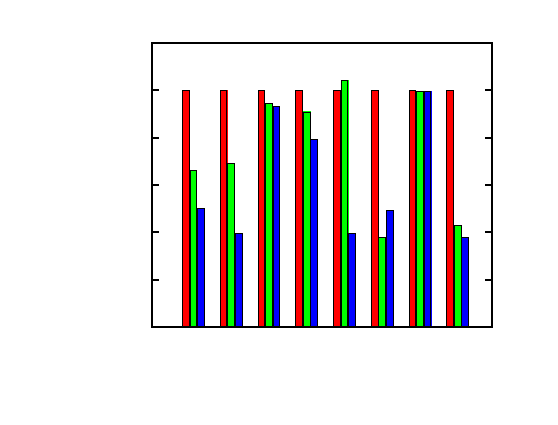
\includegraphics{numdist_query}}%
    \gplfronttext
  \end{picture}%
\endgroup
}
%}
\subfigure[]{\small
\resizebox{2.5in}{2in}{% GNUPLOT: LaTeX picture with Postscript
\begingroup
  \makeatletter
  \providecommand\color[2][]{%
    \GenericError{(gnuplot) \space\space\space\@spaces}{%
      Package color not loaded in conjunction with
      terminal option `colourtext'%
    }{See the gnuplot documentation for explanation.%
    }{Either use 'blacktext' in gnuplot or load the package
      color.sty in LaTeX.}%
    \renewcommand\color[2][]{}%
  }%
  \providecommand\includegraphics[2][]{%
    \GenericError{(gnuplot) \space\space\space\@spaces}{%
      Package graphicx or graphics not loaded%
    }{See the gnuplot documentation for explanation.%
    }{The gnuplot epslatex terminal needs graphicx.sty or graphics.sty.}%
    \renewcommand\includegraphics[2][]{}%
  }%
  \providecommand\rotatebox[2]{#2}%
  \@ifundefined{ifGPcolor}{%
    \newif\ifGPcolor
    \GPcolortrue
  }{}%
  \@ifundefined{ifGPblacktext}{%
    \newif\ifGPblacktext
    \GPblacktextfalse
  }{}%
  % define a \g@addto@macro without @ in the name:
  \let\gplgaddtomacro\g@addto@macro
  % define empty templates for all commands taking text:
  \gdef\gplbacktext{}%
  \gdef\gplfronttext{}%
  \makeatother
  \ifGPblacktext
    % no textcolor at all
    \def\colorrgb#1{}%
    \def\colorgray#1{}%
  \else
    % gray or color?
    \ifGPcolor
      \def\colorrgb#1{\color[rgb]{#1}}%
      \def\colorgray#1{\color[gray]{#1}}%
      \expandafter\def\csname LTw\endcsname{\color{white}}%
      \expandafter\def\csname LTb\endcsname{\color{black}}%
      \expandafter\def\csname LTa\endcsname{\color{black}}%
      \expandafter\def\csname LT0\endcsname{\color[rgb]{1,0,0}}%
      \expandafter\def\csname LT1\endcsname{\color[rgb]{0,1,0}}%
      \expandafter\def\csname LT2\endcsname{\color[rgb]{0,0,1}}%
      \expandafter\def\csname LT3\endcsname{\color[rgb]{1,0,1}}%
      \expandafter\def\csname LT4\endcsname{\color[rgb]{0,1,1}}%
      \expandafter\def\csname LT5\endcsname{\color[rgb]{1,1,0}}%
      \expandafter\def\csname LT6\endcsname{\color[rgb]{0,0,0}}%
      \expandafter\def\csname LT7\endcsname{\color[rgb]{1,0.3,0}}%
      \expandafter\def\csname LT8\endcsname{\color[rgb]{0.5,0.5,0.5}}%
    \else
      % gray
      \def\colorrgb#1{\color{black}}%
      \def\colorgray#1{\color[gray]{#1}}%
      \expandafter\def\csname LTw\endcsname{\color{white}}%
      \expandafter\def\csname LTb\endcsname{\color{black}}%
      \expandafter\def\csname LTa\endcsname{\color{black}}%
      \expandafter\def\csname LT0\endcsname{\color{black}}%
      \expandafter\def\csname LT1\endcsname{\color{black}}%
      \expandafter\def\csname LT2\endcsname{\color{black}}%
      \expandafter\def\csname LT3\endcsname{\color{black}}%
      \expandafter\def\csname LT4\endcsname{\color{black}}%
      \expandafter\def\csname LT5\endcsname{\color{black}}%
      \expandafter\def\csname LT6\endcsname{\color{black}}%
      \expandafter\def\csname LT7\endcsname{\color{black}}%
      \expandafter\def\csname LT8\endcsname{\color{black}}%
    \fi
  \fi
  \setlength{\unitlength}{0.0500bp}%
  \begin{picture}(5040.00,3772.00)%
    \gplgaddtomacro\gplbacktext{%
      \csname LTb\endcsname%
      \put(1122,780){\makebox(0,0)[r]{\strut{} 0}}%
      \put(1122,1235){\makebox(0,0)[r]{\strut{} 1}}%
      \put(1122,1689){\makebox(0,0)[r]{\strut{} 2}}%
      \put(1122,2144){\makebox(0,0)[r]{\strut{} 3}}%
      \put(1122,2598){\makebox(0,0)[r]{\strut{} 4}}%
      \put(1122,3053){\makebox(0,0)[r]{\strut{} 5}}%
      \put(1622,648){\rotatebox{-45}{\makebox(0,0)[l]{\strut{}yearpredict}}}%
      \put(1991,648){\rotatebox{-45}{\makebox(0,0)[l]{\strut{}twitter}}}%
      \put(2359,648){\rotatebox{-45}{\makebox(0,0)[l]{\strut{}tinyImages}}}%
      \put(2728,648){\rotatebox{-45}{\makebox(0,0)[l]{\strut{}mnist}}}%
      \put(3096,648){\rotatebox{-45}{\makebox(0,0)[l]{\strut{}corel}}}%
      \put(3465,648){\rotatebox{-45}{\makebox(0,0)[l]{\strut{}covtype}}}%
      \put(3833,648){\rotatebox{-45}{\makebox(0,0)[l]{\strut{}artificial40}}}%
      \put(4202,648){\rotatebox{-45}{\makebox(0,0)[l]{\strut{}faces}}}%
      \put(176,2143){\rotatebox{-270}{\makebox(0,0){\strut{}number of distance comparisons}}}%
      \put(396,2143){\rotatebox{-270}{\makebox(0,0){\strut{}in tree \emph{construction} only}}}%
      \put(616,2143){\rotatebox{-270}{\makebox(0,0){\strut{}(normalized by the original cover tree)}}}%
      \put(2016,3205){\makebox(0,0)[l]{\strut{}19.1}}%
    }%
    \gplgaddtomacro\gplfronttext{%
    }%
    \gplbacktext
    \put(0,0){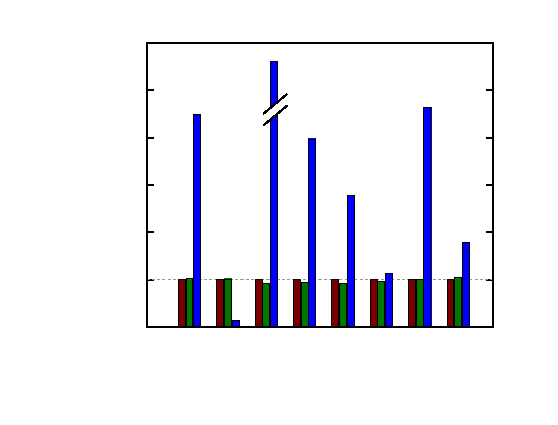
\includegraphics{img/numdist_insert}}%
    \gplfronttext
  \end{picture}%
\endgroup
}
}
\subfigure[]{\small
\resizebox{2.5in}{2in}{% GNUPLOT: LaTeX picture with Postscript
\begingroup
  \makeatletter
  \providecommand\color[2][]{%
    \GenericError{(gnuplot) \space\space\space\@spaces}{%
      Package color not loaded in conjunction with
      terminal option `colourtext'%
    }{See the gnuplot documentation for explanation.%
    }{Either use 'blacktext' in gnuplot or load the package
      color.sty in LaTeX.}%
    \renewcommand\color[2][]{}%
  }%
  \providecommand\includegraphics[2][]{%
    \GenericError{(gnuplot) \space\space\space\@spaces}{%
      Package graphicx or graphics not loaded%
    }{See the gnuplot documentation for explanation.%
    }{The gnuplot epslatex terminal needs graphicx.sty or graphics.sty.}%
    \renewcommand\includegraphics[2][]{}%
  }%
  \providecommand\rotatebox[2]{#2}%
  \@ifundefined{ifGPcolor}{%
    \newif\ifGPcolor
    \GPcolortrue
  }{}%
  \@ifundefined{ifGPblacktext}{%
    \newif\ifGPblacktext
    \GPblacktextfalse
  }{}%
  % define a \g@addto@macro without @ in the name:
  \let\gplgaddtomacro\g@addto@macro
  % define empty templates for all commands taking text:
  \gdef\gplbacktext{}%
  \gdef\gplfronttext{}%
  \makeatother
  \ifGPblacktext
    % no textcolor at all
    \def\colorrgb#1{}%
    \def\colorgray#1{}%
  \else
    % gray or color?
    \ifGPcolor
      \def\colorrgb#1{\color[rgb]{#1}}%
      \def\colorgray#1{\color[gray]{#1}}%
      \expandafter\def\csname LTw\endcsname{\color{white}}%
      \expandafter\def\csname LTb\endcsname{\color{black}}%
      \expandafter\def\csname LTa\endcsname{\color{black}}%
      \expandafter\def\csname LT0\endcsname{\color[rgb]{1,0,0}}%
      \expandafter\def\csname LT1\endcsname{\color[rgb]{0,1,0}}%
      \expandafter\def\csname LT2\endcsname{\color[rgb]{0,0,1}}%
      \expandafter\def\csname LT3\endcsname{\color[rgb]{1,0,1}}%
      \expandafter\def\csname LT4\endcsname{\color[rgb]{0,1,1}}%
      \expandafter\def\csname LT5\endcsname{\color[rgb]{1,1,0}}%
      \expandafter\def\csname LT6\endcsname{\color[rgb]{0,0,0}}%
      \expandafter\def\csname LT7\endcsname{\color[rgb]{1,0.3,0}}%
      \expandafter\def\csname LT8\endcsname{\color[rgb]{0.5,0.5,0.5}}%
    \else
      % gray
      \def\colorrgb#1{\color{black}}%
      \def\colorgray#1{\color[gray]{#1}}%
      \expandafter\def\csname LTw\endcsname{\color{white}}%
      \expandafter\def\csname LTb\endcsname{\color{black}}%
      \expandafter\def\csname LTa\endcsname{\color{black}}%
      \expandafter\def\csname LT0\endcsname{\color{black}}%
      \expandafter\def\csname LT1\endcsname{\color{black}}%
      \expandafter\def\csname LT2\endcsname{\color{black}}%
      \expandafter\def\csname LT3\endcsname{\color{black}}%
      \expandafter\def\csname LT4\endcsname{\color{black}}%
      \expandafter\def\csname LT5\endcsname{\color{black}}%
      \expandafter\def\csname LT6\endcsname{\color{black}}%
      \expandafter\def\csname LT7\endcsname{\color{black}}%
      \expandafter\def\csname LT8\endcsname{\color{black}}%
    \fi
  \fi
  \setlength{\unitlength}{0.0500bp}%
  \begin{picture}(5040.00,3772.00)%
    \gplgaddtomacro\gplbacktext{%
      \csname LTb\endcsname%
      \put(1122,780){\makebox(0,0)[r]{\strut{} 0}}%
      \put(1122,1235){\makebox(0,0)[r]{\strut{} 0.2}}%
      \put(1122,1689){\makebox(0,0)[r]{\strut{} 0.4}}%
      \put(1122,2144){\makebox(0,0)[r]{\strut{} 0.6}}%
      \put(1122,2598){\makebox(0,0)[r]{\strut{} 0.8}}%
      \put(1122,3052){\makebox(0,0)[r]{\strut{} 1}}%
      \put(1122,3507){\makebox(0,0)[r]{\strut{} 1.2}}%
      \put(1622,648){\rotatebox{-45}{\makebox(0,0)[l]{\strut{}yearpredict}}}%
      \put(1991,648){\rotatebox{-45}{\makebox(0,0)[l]{\strut{}twitter}}}%
      \put(2359,648){\rotatebox{-45}{\makebox(0,0)[l]{\strut{}tinyImages}}}%
      \put(2728,648){\rotatebox{-45}{\makebox(0,0)[l]{\strut{}mnist}}}%
      \put(3096,648){\rotatebox{-45}{\makebox(0,0)[l]{\strut{}corel}}}%
      \put(3465,648){\rotatebox{-45}{\makebox(0,0)[l]{\strut{}covtype}}}%
      \put(3833,648){\rotatebox{-45}{\makebox(0,0)[l]{\strut{}artificial40}}}%
      \put(4202,648){\rotatebox{-45}{\makebox(0,0)[l]{\strut{}faces}}}%
      \put(176,2143){\rotatebox{-270}{\makebox(0,0){\strut{}number of distance comparisons}}}%
      \put(396,2143){\rotatebox{-270}{\makebox(0,0){\strut{}in tree \emph{construction} and \emph{query}}}}%
      \put(616,2143){\rotatebox{-270}{\makebox(0,0){\strut{}(normalized by $n^2$)}}}%
    }%
    \gplgaddtomacro\gplfronttext{%
    }%
    \gplbacktext
    \put(0,0){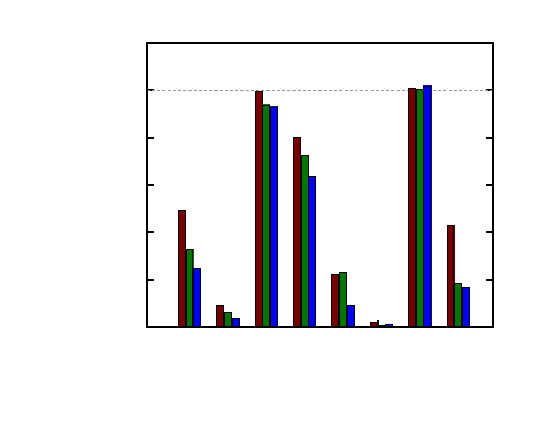
\includegraphics{img/numdist}}%
    \gplfronttext
  \end{picture}%
\endgroup
}
}
\begin{tikzpicture}
    \node[draw,fill=darkred,minimum width=0.03in,minimum height=0.3in] at (0,0) {};
    \node at (0,0.57in) {\small\rotatebox{90}{Original c.t.}};
    \node[draw,fill=darkgreen,minimum width=0.03in,minimum height=0.3in] at (0.15in,0) {};
    \node at (0.15in,0.62in) {\small\rotatebox{90}{Simplified c.t.}};
    \node[draw,fill=blue,minimum width=0.03in,minimum height=0.3in] at (0.3in,0) {};
    \node at (0.3in,0.80in) {\small\rotatebox{90}{Nearest ancestor c.t.}};
    \node[minimum width=0.05in,minimum height=0.5in] at (0.45in,0) {};
    \node at (0.45in,0.6in) {\small\rotatebox{90}{}};
    \node at (0,-0.5in) {};
\end{tikzpicture}
\caption{
    (a)
    Constructing a nearest ancestor query tree usually takes longer than the original cover tree and the simplified cover tree.
    %The extra distance comparisons come from the sorting and rebalancing steps of the nearest ancestor insertion algorithm.
    (b)
    Construction {\em plus} querying is faster in the nearest ancestor cover tree.
    On most datasets, this faster query time more than offsets the increased construction cost, giving an overall speedup.
}
\label{fig:numdist}
\end{figure*}

%%%%%%%%%%%%%%%%%%%%%%%%%%%%%%%%%%%%%%%%

\subsection{Cover tree implementation comparison}

We next compare our implementation against two good cover tree implementations currently in widespread use:
the reference implementation used in the original paper \cite{beygelzimer2006cover}
and MLPack's implementation \cite{curtin2013mlpack}.
Both of these programs were written in C++ and compiled using \texttt{g++ 4.4.7} with full optimizations.
Our implementation was written in Haskell and compiled with \texttt{ghc 7.8.4} also with full optimizations.\footnote{Our code can be downloaded at \url{http://github.com/mikeizbicki/hlearn\#covertree}.}
% cshelton1: I removed this footnote.  I don't know what we are really trying to say (even the 5-10% garbage collection doesn't mean much
%   perhaps the C++ implementation also spent 5-10% of the time reclaiming memory.  I would just let it stand as is.
%\footnote{
%Haskell has two disadvantages for performance sensitive numeric computing.
%First, it is a garbage collected language.
%In our tests, the garbage collector typically required between 5 to 10 percent of our program's run time.
%Second, Haskell only efficiently supports persistent data structures, and our cover tree is implemented persistently.
%That is, we never change the value of a variable after creation; and all previous states of the program are continuously accessible in memory.
%It is impossible to guess how persistence might affect the run time of our cover tree.
%%We implemented the cover tree in Haskell partly out of a desire to show that the language is capable of state-of-the-art performance on numerically intensive algorithms.
%}
All tests were run on an Amazon Web Services \texttt{c3.8x-large} instance with 60 GB of RAM and 32 Intel Xeon E5-2680 CPU cores clocked at 2.80GHz.
Half of those cores are hyperthreads, so for simplicity we only parallelize out to 16 cores.

Since the reference implementation and MLPack only come with the Euclidean distance built-in, we only use that metric when comparing the three implementations.
Figure \ref{fig:cache} shows the cache performance of all three libraries.
Figure \ref{fig:parallel} shows the runtime of all three libraries.
Our implementation's cache performance and parallelization speedup is shown on the nearest ancestor cover tree.
Neither the original implementation nor MLPack support parallelization.

%%%%%%%%%%%%%%%%%%%%

\begin{figure*}
\centering
\subfigure[]{\small
\resizebox{2.5in}{1.8in}{% GNUPLOT: LaTeX picture with Postscript
\begingroup
  \makeatletter
  \providecommand\color[2][]{%
    \GenericError{(gnuplot) \space\space\space\@spaces}{%
      Package color not loaded in conjunction with
      terminal option `colourtext'%
    }{See the gnuplot documentation for explanation.%
    }{Either use 'blacktext' in gnuplot or load the package
      color.sty in LaTeX.}%
    \renewcommand\color[2][]{}%
  }%
  \providecommand\includegraphics[2][]{%
    \GenericError{(gnuplot) \space\space\space\@spaces}{%
      Package graphicx or graphics not loaded%
    }{See the gnuplot documentation for explanation.%
    }{The gnuplot epslatex terminal needs graphicx.sty or graphics.sty.}%
    \renewcommand\includegraphics[2][]{}%
  }%
  \providecommand\rotatebox[2]{#2}%
  \@ifundefined{ifGPcolor}{%
    \newif\ifGPcolor
    \GPcolortrue
  }{}%
  \@ifundefined{ifGPblacktext}{%
    \newif\ifGPblacktext
    \GPblacktextfalse
  }{}%
  % define a \g@addto@macro without @ in the name:
  \let\gplgaddtomacro\g@addto@macro
  % define empty templates for all commands taking text:
  \gdef\gplbacktext{}%
  \gdef\gplfronttext{}%
  \makeatother
  \ifGPblacktext
    % no textcolor at all
    \def\colorrgb#1{}%
    \def\colorgray#1{}%
  \else
    % gray or color?
    \ifGPcolor
      \def\colorrgb#1{\color[rgb]{#1}}%
      \def\colorgray#1{\color[gray]{#1}}%
      \expandafter\def\csname LTw\endcsname{\color{white}}%
      \expandafter\def\csname LTb\endcsname{\color{black}}%
      \expandafter\def\csname LTa\endcsname{\color{black}}%
      \expandafter\def\csname LT0\endcsname{\color[rgb]{1,0,0}}%
      \expandafter\def\csname LT1\endcsname{\color[rgb]{0,1,0}}%
      \expandafter\def\csname LT2\endcsname{\color[rgb]{0,0,1}}%
      \expandafter\def\csname LT3\endcsname{\color[rgb]{1,0,1}}%
      \expandafter\def\csname LT4\endcsname{\color[rgb]{0,1,1}}%
      \expandafter\def\csname LT5\endcsname{\color[rgb]{1,1,0}}%
      \expandafter\def\csname LT6\endcsname{\color[rgb]{0,0,0}}%
      \expandafter\def\csname LT7\endcsname{\color[rgb]{1,0.3,0}}%
      \expandafter\def\csname LT8\endcsname{\color[rgb]{0.5,0.5,0.5}}%
    \else
      % gray
      \def\colorrgb#1{\color{black}}%
      \def\colorgray#1{\color[gray]{#1}}%
      \expandafter\def\csname LTw\endcsname{\color{white}}%
      \expandafter\def\csname LTb\endcsname{\color{black}}%
      \expandafter\def\csname LTa\endcsname{\color{black}}%
      \expandafter\def\csname LT0\endcsname{\color{black}}%
      \expandafter\def\csname LT1\endcsname{\color{black}}%
      \expandafter\def\csname LT2\endcsname{\color{black}}%
      \expandafter\def\csname LT3\endcsname{\color{black}}%
      \expandafter\def\csname LT4\endcsname{\color{black}}%
      \expandafter\def\csname LT5\endcsname{\color{black}}%
      \expandafter\def\csname LT6\endcsname{\color{black}}%
      \expandafter\def\csname LT7\endcsname{\color{black}}%
      \expandafter\def\csname LT8\endcsname{\color{black}}%
    \fi
  \fi
  \setlength{\unitlength}{0.0500bp}%
  \begin{picture}(5040.00,3772.00)%
    \gplgaddtomacro\gplbacktext{%
      \csname LTb\endcsname%
      \put(1166,780){\makebox(0,0)[r]{\strut{} 0}}%
      \put(1166,1325){\makebox(0,0)[r]{\strut{} 0.2}}%
      \put(1166,1871){\makebox(0,0)[r]{\strut{} 0.4}}%
      \put(1166,2416){\makebox(0,0)[r]{\strut{} 0.6}}%
      \put(1166,2962){\makebox(0,0)[r]{\strut{} 0.8}}%
      \put(1166,3507){\makebox(0,0)[r]{\strut{} 1}}%
      \put(1661,648){\rotatebox{-45}{\makebox(0,0)[l]{\strut{}yearpredict}}}%
      \put(2023,648){\rotatebox{-45}{\makebox(0,0)[l]{\strut{}twitter}}}%
      \put(2386,648){\rotatebox{-45}{\makebox(0,0)[l]{\strut{}tinyImages}}}%
      \put(2748,648){\rotatebox{-45}{\makebox(0,0)[l]{\strut{}mnist}}}%
      \put(3111,648){\rotatebox{-45}{\makebox(0,0)[l]{\strut{}corel}}}%
      \put(3473,648){\rotatebox{-45}{\makebox(0,0)[l]{\strut{}covtype}}}%
      \put(3836,648){\rotatebox{-45}{\makebox(0,0)[l]{\strut{}artificial40}}}%
      \put(4198,648){\rotatebox{-45}{\makebox(0,0)[l]{\strut{}faces}}}%
      \put(176,2143){\rotatebox{-270}{\makebox(0,0){\strut{}cache miss rate}}}%
      \put(396,2143){\rotatebox{-270}{\makebox(0,0){\strut{}(cache misses / cache accesses)}}}%
    }%
    \gplgaddtomacro\gplfronttext{%
    }%
    \gplbacktext
    \put(0,0){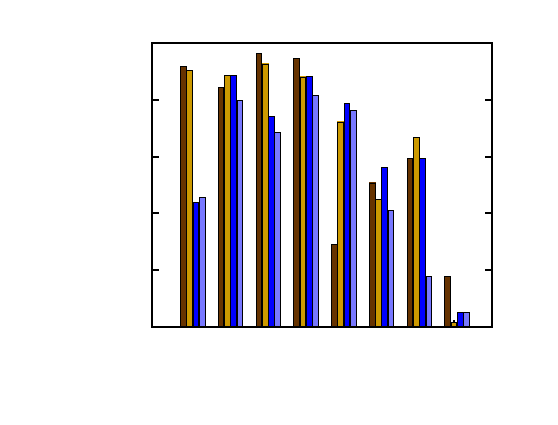
\includegraphics{img/cache}}%
    \gplfronttext
  \end{picture}%
\endgroup
}
}
\subfigure[]{\small
\resizebox{2.5in}{1.8in}{% GNUPLOT: LaTeX picture with Postscript
\begingroup
  \makeatletter
  \providecommand\color[2][]{%
    \GenericError{(gnuplot) \space\space\space\@spaces}{%
      Package color not loaded in conjunction with
      terminal option `colourtext'%
    }{See the gnuplot documentation for explanation.%
    }{Either use 'blacktext' in gnuplot or load the package
      color.sty in LaTeX.}%
    \renewcommand\color[2][]{}%
  }%
  \providecommand\includegraphics[2][]{%
    \GenericError{(gnuplot) \space\space\space\@spaces}{%
      Package graphicx or graphics not loaded%
    }{See the gnuplot documentation for explanation.%
    }{The gnuplot epslatex terminal needs graphicx.sty or graphics.sty.}%
    \renewcommand\includegraphics[2][]{}%
  }%
  \providecommand\rotatebox[2]{#2}%
  \@ifundefined{ifGPcolor}{%
    \newif\ifGPcolor
    \GPcolortrue
  }{}%
  \@ifundefined{ifGPblacktext}{%
    \newif\ifGPblacktext
    \GPblacktextfalse
  }{}%
  % define a \g@addto@macro without @ in the name:
  \let\gplgaddtomacro\g@addto@macro
  % define empty templates for all commands taking text:
  \gdef\gplbacktext{}%
  \gdef\gplfronttext{}%
  \makeatother
  \ifGPblacktext
    % no textcolor at all
    \def\colorrgb#1{}%
    \def\colorgray#1{}%
  \else
    % gray or color?
    \ifGPcolor
      \def\colorrgb#1{\color[rgb]{#1}}%
      \def\colorgray#1{\color[gray]{#1}}%
      \expandafter\def\csname LTw\endcsname{\color{white}}%
      \expandafter\def\csname LTb\endcsname{\color{black}}%
      \expandafter\def\csname LTa\endcsname{\color{black}}%
      \expandafter\def\csname LT0\endcsname{\color[rgb]{1,0,0}}%
      \expandafter\def\csname LT1\endcsname{\color[rgb]{0,1,0}}%
      \expandafter\def\csname LT2\endcsname{\color[rgb]{0,0,1}}%
      \expandafter\def\csname LT3\endcsname{\color[rgb]{1,0,1}}%
      \expandafter\def\csname LT4\endcsname{\color[rgb]{0,1,1}}%
      \expandafter\def\csname LT5\endcsname{\color[rgb]{1,1,0}}%
      \expandafter\def\csname LT6\endcsname{\color[rgb]{0,0,0}}%
      \expandafter\def\csname LT7\endcsname{\color[rgb]{1,0.3,0}}%
      \expandafter\def\csname LT8\endcsname{\color[rgb]{0.5,0.5,0.5}}%
    \else
      % gray
      \def\colorrgb#1{\color{black}}%
      \def\colorgray#1{\color[gray]{#1}}%
      \expandafter\def\csname LTw\endcsname{\color{white}}%
      \expandafter\def\csname LTb\endcsname{\color{black}}%
      \expandafter\def\csname LTa\endcsname{\color{black}}%
      \expandafter\def\csname LT0\endcsname{\color{black}}%
      \expandafter\def\csname LT1\endcsname{\color{black}}%
      \expandafter\def\csname LT2\endcsname{\color{black}}%
      \expandafter\def\csname LT3\endcsname{\color{black}}%
      \expandafter\def\csname LT4\endcsname{\color{black}}%
      \expandafter\def\csname LT5\endcsname{\color{black}}%
      \expandafter\def\csname LT6\endcsname{\color{black}}%
      \expandafter\def\csname LT7\endcsname{\color{black}}%
      \expandafter\def\csname LT8\endcsname{\color{black}}%
    \fi
  \fi
  \setlength{\unitlength}{0.0500bp}%
  \begin{picture}(5040.00,3772.00)%
    \gplgaddtomacro\gplbacktext{%
      \csname LTb\endcsname%
      \put(1166,780){\makebox(0,0)[r]{\strut{} 0}}%
      \put(1166,1325){\makebox(0,0)[r]{\strut{} 0.2}}%
      \put(1166,1871){\makebox(0,0)[r]{\strut{} 0.4}}%
      \put(1166,2416){\makebox(0,0)[r]{\strut{} 0.6}}%
      \put(1166,2962){\makebox(0,0)[r]{\strut{} 0.8}}%
      \put(1166,3507){\makebox(0,0)[r]{\strut{} 1}}%
      \put(1661,648){\rotatebox{-45}{\makebox(0,0)[l]{\strut{}yearpredict}}}%
      \put(2023,648){\rotatebox{-45}{\makebox(0,0)[l]{\strut{}twitter}}}%
      \put(2386,648){\rotatebox{-45}{\makebox(0,0)[l]{\strut{}tinyImages}}}%
      \put(2748,648){\rotatebox{-45}{\makebox(0,0)[l]{\strut{}mnist}}}%
      \put(3111,648){\rotatebox{-45}{\makebox(0,0)[l]{\strut{}corel}}}%
      \put(3473,648){\rotatebox{-45}{\makebox(0,0)[l]{\strut{}covtype}}}%
      \put(3836,648){\rotatebox{-45}{\makebox(0,0)[l]{\strut{}artificial40}}}%
      \put(4198,648){\rotatebox{-45}{\makebox(0,0)[l]{\strut{}faces}}}%
      \put(176,2143){\rotatebox{-270}{\makebox(0,0){\strut{}stalled CPU cycle rate}}}%
      \put(396,2143){\rotatebox{-270}{\makebox(0,0){\strut{}(stalled cycles / total cycles)}}}%
    }%
    \gplgaddtomacro\gplfronttext{%
    }%
    \gplbacktext
    \put(0,0){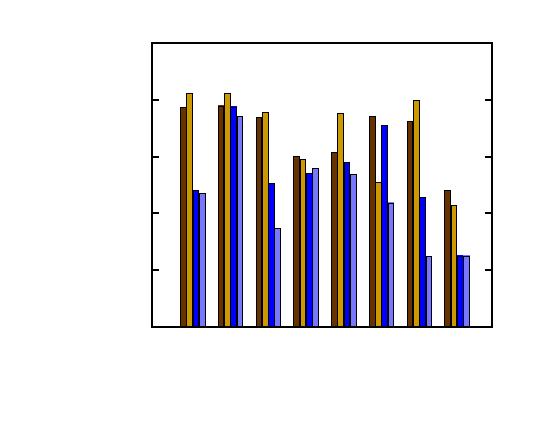
\includegraphics{img/stalled-front}}%
    \gplfronttext
  \end{picture}%
\endgroup
}
}
\definecolor{colorOrig}{RGB}{102,51,0}
\definecolor{colorMlpack}{RGB}{204,153,0}
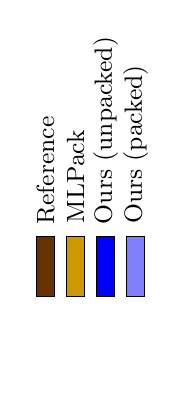
\begin{tikzpicture}
    \node[draw,fill=colorOrig,minimum width=0.05in,minimum height=0.3in] at (0,0) {};
    \node at (0,0.48in) {\small\rotatebox{90}{Reference}};
    \node[draw,fill=colorMlpack,minimum width=0.05in,minimum height=0.3in] at (0.15in,0) {};
    \node at (0.15in,0.45in) {\small\rotatebox{90}{MLPack}};
    \node[draw,fill=blue,minimum width=0.05in,minimum height=0.3in] at (0.3in,0) {};
    \node at (0.3in,0.68in) {\small\rotatebox{90}{Ours (unpacked)}};
    \node[draw,fill=lightblue,minimum width=0.05in,minimum height=0.3in] at (0.45in,0) {};
    \node at (0.45in,0.61in) {\small\rotatebox{90}{Ours (packed)}};
    \node at (0,-0.475in) {};
\end{tikzpicture}
\caption{
    (a)
	Comparison of our packed nearest ancestor cover tree to our unpacked tree and other implementations, demonstrating better cache performance.
    %Our packed cover tree has better cache performance than our unpacked cover tree, and usually has better cache performance than the other two implementations.
    (b)
    A stalled CPU cycle is when the CPU does no work because it must wait for a memory access. %can do no work processing an instruction because it must wait on data to be retrieved from memory.
    Reducing the number of cache misses results in fewer stalled cycles, and so faster run times.
    We used the Linux \mkprocedure{perf stat} utility to measure the \mkprocedure{cache-references}, \mkprocedure{cache-misses}, \mkprocedure{cycles}, and \mkprocedure{stalled-cycles-frontend} hardware counters.
    \mkprocedure{perf stat} uses a sampling strategy with negligible affect on program performance.
    %(a)
    %Our packed cover tree always has better cache performance than our unpacked cover tree, and usually has better cache performance than the other two implementations.
    %For this experiment, the Linux \mkprocedure{perf stat} utility was used to measure the \mkprocedure{cache-references} and \mkprocedure{cache-misses} hardware counters.
    %This corresponds to the cache level closest to memory (i.e. the Last Level Cache).
    %\mkprocedure{perf stat} uses a sampling strategy that has a negligible affect on the program's actual performance.
    %(b)
    %A stalled CPU cycle is one where the CPU can do no work processing an instruction because it must wait on data to be retrieved from memory.
    %Reducing the number of cache misses results in fewer stalled cycles, and so faster run times.
    %Measurements are from the \mkprocedure{cycles} and \mkprocedure{stalled-cycles-frontend} hardware counters.
    }
\label{fig:cache}
\end{figure*}

%%%%%%%%%%%%%%%%%%%%

\begin{figure*}
\centering
\subfigure[]{\small
\resizebox{2.5in}{1.8in}{% GNUPLOT: LaTeX picture with Postscript
\begingroup
  \makeatletter
  \providecommand\color[2][]{%
    \GenericError{(gnuplot) \space\space\space\@spaces}{%
      Package color not loaded in conjunction with
      terminal option `colourtext'%
    }{See the gnuplot documentation for explanation.%
    }{Either use 'blacktext' in gnuplot or load the package
      color.sty in LaTeX.}%
    \renewcommand\color[2][]{}%
  }%
  \providecommand\includegraphics[2][]{%
    \GenericError{(gnuplot) \space\space\space\@spaces}{%
      Package graphicx or graphics not loaded%
    }{See the gnuplot documentation for explanation.%
    }{The gnuplot epslatex terminal needs graphicx.sty or graphics.sty.}%
    \renewcommand\includegraphics[2][]{}%
  }%
  \providecommand\rotatebox[2]{#2}%
  \@ifundefined{ifGPcolor}{%
    \newif\ifGPcolor
    \GPcolortrue
  }{}%
  \@ifundefined{ifGPblacktext}{%
    \newif\ifGPblacktext
    \GPblacktextfalse
  }{}%
  % define a \g@addto@macro without @ in the name:
  \let\gplgaddtomacro\g@addto@macro
  % define empty templates for all commands taking text:
  \gdef\gplbacktext{}%
  \gdef\gplfronttext{}%
  \makeatother
  \ifGPblacktext
    % no textcolor at all
    \def\colorrgb#1{}%
    \def\colorgray#1{}%
  \else
    % gray or color?
    \ifGPcolor
      \def\colorrgb#1{\color[rgb]{#1}}%
      \def\colorgray#1{\color[gray]{#1}}%
      \expandafter\def\csname LTw\endcsname{\color{white}}%
      \expandafter\def\csname LTb\endcsname{\color{black}}%
      \expandafter\def\csname LTa\endcsname{\color{black}}%
      \expandafter\def\csname LT0\endcsname{\color[rgb]{1,0,0}}%
      \expandafter\def\csname LT1\endcsname{\color[rgb]{0,1,0}}%
      \expandafter\def\csname LT2\endcsname{\color[rgb]{0,0,1}}%
      \expandafter\def\csname LT3\endcsname{\color[rgb]{1,0,1}}%
      \expandafter\def\csname LT4\endcsname{\color[rgb]{0,1,1}}%
      \expandafter\def\csname LT5\endcsname{\color[rgb]{1,1,0}}%
      \expandafter\def\csname LT6\endcsname{\color[rgb]{0,0,0}}%
      \expandafter\def\csname LT7\endcsname{\color[rgb]{1,0.3,0}}%
      \expandafter\def\csname LT8\endcsname{\color[rgb]{0.5,0.5,0.5}}%
    \else
      % gray
      \def\colorrgb#1{\color{black}}%
      \def\colorgray#1{\color[gray]{#1}}%
      \expandafter\def\csname LTw\endcsname{\color{white}}%
      \expandafter\def\csname LTb\endcsname{\color{black}}%
      \expandafter\def\csname LTa\endcsname{\color{black}}%
      \expandafter\def\csname LT0\endcsname{\color{black}}%
      \expandafter\def\csname LT1\endcsname{\color{black}}%
      \expandafter\def\csname LT2\endcsname{\color{black}}%
      \expandafter\def\csname LT3\endcsname{\color{black}}%
      \expandafter\def\csname LT4\endcsname{\color{black}}%
      \expandafter\def\csname LT5\endcsname{\color{black}}%
      \expandafter\def\csname LT6\endcsname{\color{black}}%
      \expandafter\def\csname LT7\endcsname{\color{black}}%
      \expandafter\def\csname LT8\endcsname{\color{black}}%
    \fi
  \fi
  \setlength{\unitlength}{0.0500bp}%
  \begin{picture}(5040.00,3772.00)%
    \gplgaddtomacro\gplbacktext{%
      \csname LTb\endcsname%
      \put(814,1129){\makebox(0,0)[r]{\strut{}$2^{-4}$}}%
      \csname LTb\endcsname%
      \put(814,1526){\makebox(0,0)[r]{\strut{}$2^{-3}$}}%
      \csname LTb\endcsname%
      \put(814,1922){\makebox(0,0)[r]{\strut{}$2^{-2}$}}%
      \csname LTb\endcsname%
      \put(814,2318){\makebox(0,0)[r]{\strut{}$2^{-1}$}}%
      \csname LTb\endcsname%
      \put(814,2714){\makebox(0,0)[r]{\strut{}$2^{+0}$}}%
      \csname LTb\endcsname%
      \put(814,3111){\makebox(0,0)[r]{\strut{}$2^{+1}$}}%
      \put(1539,601){\rotatebox{-45}{\makebox(0,0)[l]{\strut{}yearpredict}}}%
      \put(1539,381){\rotatebox{-45}{\makebox(0,0)[l]{\strut{}(77sec)}}}%
      \put(2242,601){\rotatebox{-45}{\makebox(0,0)[l]{\strut{}twitter}}}%
      \put(2242,381){\rotatebox{-45}{\makebox(0,0)[l]{\strut{}(107sec)}}}%
      \put(2945,601){\rotatebox{-45}{\makebox(0,0)[l]{\strut{}tinyImages}}}%
      \put(2945,381){\rotatebox{-45}{\makebox(0,0)[l]{\strut{}(65sec)}}}%
      \put(3648,601){\rotatebox{-45}{\makebox(0,0)[l]{\strut{}mnist}}}%
      \put(3648,381){\rotatebox{-45}{\makebox(0,0)[l]{\strut{}(12sec)}}}%
      \put(176,2120){\rotatebox{-270}{\makebox(0,0){\strut{}normalized tree \emph{construction} time}}}%
      \put(1464,2814){\makebox(0,0)[l]{\strut{}\tiny 1}}%
      \put(1570,2619){\makebox(0,0)[l]{\strut{}\tiny 2}}%
      \put(1667,2175){\makebox(0,0)[l]{\strut{}\tiny 4}}%
      \put(1763,1967){\makebox(0,0)[l]{\strut{}\tiny 8}}%
      \put(1860,1856){\makebox(0,0)[l]{\strut{}\tiny 16}}%
      \put(1473,3230){\makebox(0,0)[l]{\strut{}number of processors}}%
    }%
    \gplgaddtomacro\gplfronttext{%
    }%
    \gplbacktext
    \put(0,0){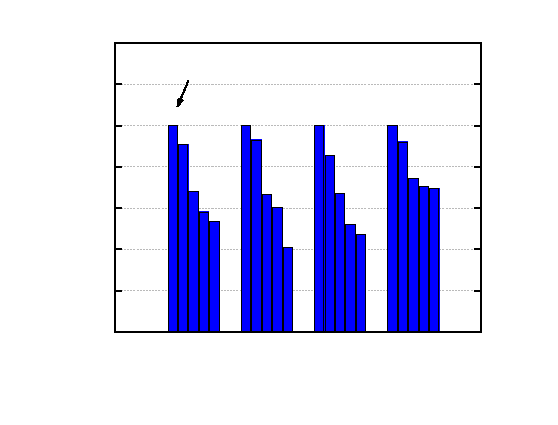
\includegraphics{img/parallel-ancestor-build}}%
    \gplfronttext
  \end{picture}%
\endgroup
}
}
\subfigure[]{\small
\resizebox{2.5in}{1.8in}{% GNUPLOT: LaTeX picture with Postscript
\begingroup
  \makeatletter
  \providecommand\color[2][]{%
    \GenericError{(gnuplot) \space\space\space\@spaces}{%
      Package color not loaded in conjunction with
      terminal option `colourtext'%
    }{See the gnuplot documentation for explanation.%
    }{Either use 'blacktext' in gnuplot or load the package
      color.sty in LaTeX.}%
    \renewcommand\color[2][]{}%
  }%
  \providecommand\includegraphics[2][]{%
    \GenericError{(gnuplot) \space\space\space\@spaces}{%
      Package graphicx or graphics not loaded%
    }{See the gnuplot documentation for explanation.%
    }{The gnuplot epslatex terminal needs graphicx.sty or graphics.sty.}%
    \renewcommand\includegraphics[2][]{}%
  }%
  \providecommand\rotatebox[2]{#2}%
  \@ifundefined{ifGPcolor}{%
    \newif\ifGPcolor
    \GPcolortrue
  }{}%
  \@ifundefined{ifGPblacktext}{%
    \newif\ifGPblacktext
    \GPblacktextfalse
  }{}%
  % define a \g@addto@macro without @ in the name:
  \let\gplgaddtomacro\g@addto@macro
  % define empty templates for all commands taking text:
  \gdef\gplbacktext{}%
  \gdef\gplfronttext{}%
  \makeatother
  \ifGPblacktext
    % no textcolor at all
    \def\colorrgb#1{}%
    \def\colorgray#1{}%
  \else
    % gray or color?
    \ifGPcolor
      \def\colorrgb#1{\color[rgb]{#1}}%
      \def\colorgray#1{\color[gray]{#1}}%
      \expandafter\def\csname LTw\endcsname{\color{white}}%
      \expandafter\def\csname LTb\endcsname{\color{black}}%
      \expandafter\def\csname LTa\endcsname{\color{black}}%
      \expandafter\def\csname LT0\endcsname{\color[rgb]{1,0,0}}%
      \expandafter\def\csname LT1\endcsname{\color[rgb]{0,1,0}}%
      \expandafter\def\csname LT2\endcsname{\color[rgb]{0,0,1}}%
      \expandafter\def\csname LT3\endcsname{\color[rgb]{1,0,1}}%
      \expandafter\def\csname LT4\endcsname{\color[rgb]{0,1,1}}%
      \expandafter\def\csname LT5\endcsname{\color[rgb]{1,1,0}}%
      \expandafter\def\csname LT6\endcsname{\color[rgb]{0,0,0}}%
      \expandafter\def\csname LT7\endcsname{\color[rgb]{1,0.3,0}}%
      \expandafter\def\csname LT8\endcsname{\color[rgb]{0.5,0.5,0.5}}%
    \else
      % gray
      \def\colorrgb#1{\color{black}}%
      \def\colorgray#1{\color[gray]{#1}}%
      \expandafter\def\csname LTw\endcsname{\color{white}}%
      \expandafter\def\csname LTb\endcsname{\color{black}}%
      \expandafter\def\csname LTa\endcsname{\color{black}}%
      \expandafter\def\csname LT0\endcsname{\color{black}}%
      \expandafter\def\csname LT1\endcsname{\color{black}}%
      \expandafter\def\csname LT2\endcsname{\color{black}}%
      \expandafter\def\csname LT3\endcsname{\color{black}}%
      \expandafter\def\csname LT4\endcsname{\color{black}}%
      \expandafter\def\csname LT5\endcsname{\color{black}}%
      \expandafter\def\csname LT6\endcsname{\color{black}}%
      \expandafter\def\csname LT7\endcsname{\color{black}}%
      \expandafter\def\csname LT8\endcsname{\color{black}}%
    \fi
  \fi
  \setlength{\unitlength}{0.0500bp}%
  \begin{picture}(5040.00,3772.00)%
    \gplgaddtomacro\gplbacktext{%
      \csname LTb\endcsname%
      \put(1254,1129){\makebox(0,0)[r]{\strut{}$2^{-4}$}}%
      \csname LTb\endcsname%
      \put(1254,1526){\makebox(0,0)[r]{\strut{}$2^{-3}$}}%
      \csname LTb\endcsname%
      \put(1254,1922){\makebox(0,0)[r]{\strut{}$2^{-2}$}}%
      \csname LTb\endcsname%
      \put(1254,2318){\makebox(0,0)[r]{\strut{}$2^{-1}$}}%
      \csname LTb\endcsname%
      \put(1254,2714){\makebox(0,0)[r]{\strut{}$2^{+0}$}}%
      \csname LTb\endcsname%
      \put(1254,3111){\makebox(0,0)[r]{\strut{}$2^{+1}$}}%
      \put(1873,601){\rotatebox{-45}{\makebox(0,0)[l]{\strut{}yearpredict}}}%
      \put(1873,381){\rotatebox{-45}{\makebox(0,0)[l]{\strut{}(277min)}}}%
      \put(2471,601){\rotatebox{-45}{\makebox(0,0)[l]{\strut{}twitter}}}%
      \put(2471,381){\rotatebox{-45}{\makebox(0,0)[l]{\strut{}(51min)}}}%
      \put(3068,601){\rotatebox{-45}{\makebox(0,0)[l]{\strut{}tinyImages}}}%
      \put(3068,381){\rotatebox{-45}{\makebox(0,0)[l]{\strut{}(34min)}}}%
      \put(3666,601){\rotatebox{-45}{\makebox(0,0)[l]{\strut{}mnist}}}%
      \put(3666,381){\rotatebox{-45}{\makebox(0,0)[l]{\strut{}(30min)}}}%
      \put(176,2120){\rotatebox{-270}{\makebox(0,0){\strut{}normalized total runtime}}}%
      \put(396,2120){\rotatebox{-270}{\makebox(0,0){\strut{}(both \emph{construction} and \emph{query})}}}%
      \put(616,2120){\rotatebox{-270}{\makebox(0,0){\strut{}  }}}%
      \put(1774,2980){\makebox(0,0)[l]{\strut{}\tiny 1}}%
      \put(1849,3174){\makebox(0,0)[l]{\strut{}\tiny 1}}%
      \put(1924,2814){\makebox(0,0)[l]{\strut{}\tiny 1}}%
      \put(1983,2453){\makebox(0,0)[l]{\strut{}\tiny 2}}%
      \put(2058,1954){\makebox(0,0)[l]{\strut{}\tiny 4}}%
      \put(2124,1648){\makebox(0,0)[l]{\strut{}\tiny 8}}%
      \put(2184,1399){\makebox(0,0)[l]{\strut{}\tiny 16}}%
    }%
    \gplgaddtomacro\gplfronttext{%
    }%
    \gplbacktext
    \put(0,0){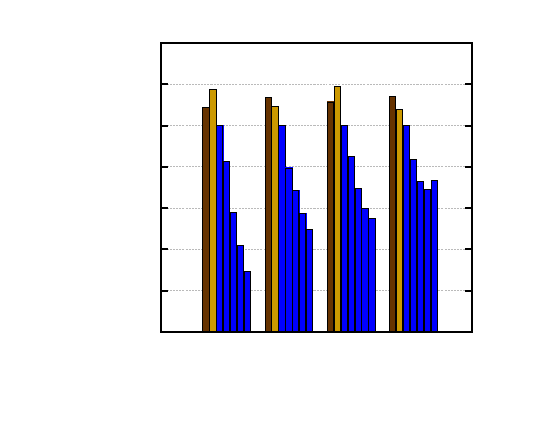
\includegraphics{img/parallel}}%
    \gplfronttext
  \end{picture}%
\endgroup
}
}
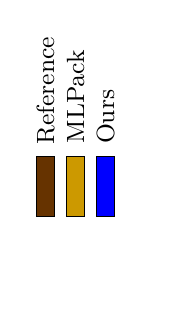
\begin{tikzpicture}
    \node[draw,fill=colorOrig,minimum width=0.05in,minimum height=0.3in] at (0,0) {};
    \node at (0,0.48in) {\small\rotatebox{90}{Reference}};
    \node[draw,fill=colorMlpack,minimum width=0.05in,minimum height=0.3in] at (0.15in,0) {};
    \node at (0.15in,0.45in) {\small\rotatebox{90}{MLPack}};
    \node[draw,fill=blue,minimum width=0.05in,minimum height=0.3in] at (0.3in,0) {};
    \node at (0.3in,0.35in) {\small\rotatebox{90}{Ours}};
    \node[minimum width=0.05in,minimum height=0.3in] at (0.45in,0) {};
    \node at (0.45in,0.61in) {\small\rotatebox{90}{}};
    \node at (0,-0.475in) {};
\end{tikzpicture}
\caption{
    Run times on the ``all nearest neighbor'' procedure for only those datasets that take more than 5 minutes.
    (a) Tree construction. %The effectiveness of parallelization on tree construction.
    A single cover tree merge takes about 1\% of the computation time;
    the main reason for the lack of perfect parallel speedup is the increased number of cache misses caused by inserting into multiple trees simultaneously.
    (b) Comparison on total performance to reference and MLPack implementations. %This figure shows the overall effectiveness of parallelization, and compares our runtimes with those of the reference implementation and MLPack implementation of cover trees.
    Runtimes in both figures are divided by that of our single processor implementation (shown in parenthesis).
    }
\label{fig:parallel}
\end{figure*}

%%%%%%%%%%%%%%%%%%%%%%%%%%%%%%%%%%%%%%%%

\subsection{Alternative methods for Euclidean nearest neighbors}

Next we compare our cover tree implementation to non-cover tree based nearest neighbor libraries.
Specifically, we compare to a $k$d-tree implemented in the Fast Library for Approximate Nearest Neighbor \citep[FLANN; ][]{muja2014scalable},
a $k$d-tree implemented in Julia \citep{bezanson2017julia},
the original cover tree implementation \citep{beygelzimer2006cover},
a $k$d-tree and cover tree implemented in MLPack \citep{curtin2013mlpack},
a $k$d-tree and ball tree implemented in Python's scikit learn \citep{scikit-learn},
and a $k$d-tree implemented in R \citep{R}.
The results are shown in Figures \ref{fig:allexp1} and \ref{allexp2}.
Without parallelization, our implementation is faster than most of the alternatives on most of the datasets.
With parallelization it is faster than all of the alternatives on all of the datasets.

\begin{figure}
    \begin{tabular}{cc}
    \includegraphics[width=.45\textwidth]{img-website/mnist}
    &
    \includegraphics[width=.45\textwidth]{img-website/tinyImages}
    \\
    \includegraphics[width=.45\textwidth]{img-website/twitter}
    &
    \includegraphics[width=.45\textwidth]{img-website/yearpredict}
    \end{tabular}
    \caption{
Using only a single processor, 
our nearest ancestor cover tree performs the fastest on each dataset except for YearPredict.
%But HLearn can use all the cores on your computer to parallelize the task.
%Here's how performance scales with the number of CPUs on an AWS EC2 `c3.8xlarge` instance with 16 true cores:
    }
    \label{fig:allexp1}
\end{figure}

\begin{figure}
    \centering
    \includegraphics[width=.5\textwidth]{img-website/yearpredict-parallel}
    \caption{
        Using multiple processors, 
        our implementation is now also the fastest on the YearPredict dataset by a wide margin.
        (FLANN is the only other library supporting parallelism, 
        but in my tests with this dataset parallelism actually slowed it down for some reason.)
    }
    \label{fig:allexp2}
\end{figure}

%%%%%%%%%%%%%%%%%%%%%%%%%%%%%%%%%%%%%%%%

\subsection{Graph kernels and protein function}

An important problem in bioinformatics is to predict the function of a protein based on its 3d structure.
State of the art solutions model the protein's 3d structure as a graph and use support vector machines (with a graph kernel) for prediction.
Computing graph kernels is relatively expensive, however, so research has focused on making the graph kernel computation faster \citep{Vishwanathan2010,Shervashidze2011}.
Such research makes graph kernels scale to \emph{larger graphs}, but does not help in the case where there are \emph{more graphs}.
Our contribution is to use cover trees to reduce the number of required kernel computations, letting us scale to more graphs.
The largest dataset in previous research contained about 1200 proteins.
With our cover tree, we perform nearest neighbor queries on all one hundred thousand proteins currently registered in the Protein Data Bank \citep{Berman2000}.

We use the random walk graph kernel in our experiment.
It performs well on protein classification and is conceptually simple.
%The random walk kernel between graphs $A$ and $B$ is defined as:
%$$
%k(A,B) = \sum_{i=1}^\infty \lambda_i (p_A \otimes p_B)^\intercal (A \otimes B)^i (q_A \otimes q_B)
%$$
%where: the scalar $\lambda_i$ controls the relative importance of walks of length $i$;
%the variables $A$ and $B$ are overloaded to also denote the adjacency matrix of the corresponding graph;
%the dimensions of $A$ and $B$ are $n \times n$ and $m \times m$ respectively;
%the vectors $p_A$, $q_A$, $p_B$ and $q_B$ have lengths $n$, $n$, $m$, and $m$ and all sum to 1;
%the $j$th element of $p_A$ corresponds to the probability of starting  the random walk at node $j$ in graph $A$;
%the entries of $q$ similarly represent the probability of stopping at each node.
See \citet{Vishwanathan2010} for more details.
A naive computation of this kernel takes time $O(v^6)$, where $v$ is the number of vertices in the graph.
\citet{Vishwanathan2010} present faster methods that take time only $O(v^3)$.
While considerably faster, it is still a relatively expensive distance computation.
%For use with the cover tree, we convert the random walk graph kernel into a distance metric using the standard formula:
%$$
%d(A,B) = \sqrt{k(A,A) + k(B,B) -2k(A,B)}
%$$

The Protein Data Bank \cite{Berman2000} contains information on the 3d primary structure of approximately one hundred thousand proteins.
To perform our experiment, we follow a procedure similar to that used by the PROTEIN dataset used in the experiments in \citet{Vishwanathan2010}.
This procedure constructs secondary structure graphs from the primary structures in the Protein Data Bank
using the tool VLPG \citep{Schfer2012}.
The Protein Data Bank stores the 3d structure of the atoms in the protein in a PDB file.
From this PDB file, we calculate the protein's secondary structure using the DSSP tool \citep{Joosten11}.
Then, the tool VLPG \citep{Schfer2012} generates graphs from the resulting secondary structure.
Some PDB files contain information for multiple graphs, and some do not contain enough information to construct a graph.
In total, our dataset consists of 250,000 graphs, and a typical graph has between 5-120 nodes and 0.1-3 edges per node.
Figure \ref{fig:bio} shows the scaling behavior of all three cover trees on this dataset.
On all of the data, the total construction and query cost are $29$\% that of the original cover tree.

\begin{figure}[t]
\centering
%\resizebox{\columnwidth}{2in}{% GNUPLOT: LaTeX picture with Postscript
\begingroup
  \makeatletter
  \providecommand\color[2][]{%
    \GenericError{(gnuplot) \space\space\space\@spaces}{%
      Package color not loaded in conjunction with
      terminal option `colourtext'%
    }{See the gnuplot documentation for explanation.%
    }{Either use 'blacktext' in gnuplot or load the package
      color.sty in LaTeX.}%
    \renewcommand\color[2][]{}%
  }%
  \providecommand\includegraphics[2][]{%
    \GenericError{(gnuplot) \space\space\space\@spaces}{%
      Package graphicx or graphics not loaded%
    }{See the gnuplot documentation for explanation.%
    }{The gnuplot epslatex terminal needs graphicx.sty or graphics.sty.}%
    \renewcommand\includegraphics[2][]{}%
  }%
  \providecommand\rotatebox[2]{#2}%
  \@ifundefined{ifGPcolor}{%
    \newif\ifGPcolor
    \GPcolortrue
  }{}%
  \@ifundefined{ifGPblacktext}{%
    \newif\ifGPblacktext
    \GPblacktextfalse
  }{}%
  % define a \g@addto@macro without @ in the name:
  \let\gplgaddtomacro\g@addto@macro
  % define empty templates for all commands taking text:
  \gdef\gplbacktext{}%
  \gdef\gplfronttext{}%
  \makeatother
  \ifGPblacktext
    % no textcolor at all
    \def\colorrgb#1{}%
    \def\colorgray#1{}%
  \else
    % gray or color?
    \ifGPcolor
      \def\colorrgb#1{\color[rgb]{#1}}%
      \def\colorgray#1{\color[gray]{#1}}%
      \expandafter\def\csname LTw\endcsname{\color{white}}%
      \expandafter\def\csname LTb\endcsname{\color{black}}%
      \expandafter\def\csname LTa\endcsname{\color{black}}%
      \expandafter\def\csname LT0\endcsname{\color[rgb]{1,0,0}}%
      \expandafter\def\csname LT1\endcsname{\color[rgb]{0,1,0}}%
      \expandafter\def\csname LT2\endcsname{\color[rgb]{0,0,1}}%
      \expandafter\def\csname LT3\endcsname{\color[rgb]{1,0,1}}%
      \expandafter\def\csname LT4\endcsname{\color[rgb]{0,1,1}}%
      \expandafter\def\csname LT5\endcsname{\color[rgb]{1,1,0}}%
      \expandafter\def\csname LT6\endcsname{\color[rgb]{0,0,0}}%
      \expandafter\def\csname LT7\endcsname{\color[rgb]{1,0.3,0}}%
      \expandafter\def\csname LT8\endcsname{\color[rgb]{0.5,0.5,0.5}}%
    \else
      % gray
      \def\colorrgb#1{\color{black}}%
      \def\colorgray#1{\color[gray]{#1}}%
      \expandafter\def\csname LTw\endcsname{\color{white}}%
      \expandafter\def\csname LTb\endcsname{\color{black}}%
      \expandafter\def\csname LTa\endcsname{\color{black}}%
      \expandafter\def\csname LT0\endcsname{\color{black}}%
      \expandafter\def\csname LT1\endcsname{\color{black}}%
      \expandafter\def\csname LT2\endcsname{\color{black}}%
      \expandafter\def\csname LT3\endcsname{\color{black}}%
      \expandafter\def\csname LT4\endcsname{\color{black}}%
      \expandafter\def\csname LT5\endcsname{\color{black}}%
      \expandafter\def\csname LT6\endcsname{\color{black}}%
      \expandafter\def\csname LT7\endcsname{\color{black}}%
      \expandafter\def\csname LT8\endcsname{\color{black}}%
    \fi
  \fi
  \setlength{\unitlength}{0.0500bp}%
  \begin{picture}(5040.00,3772.00)%
    \gplgaddtomacro\gplbacktext{%
      \csname LTb\endcsname%
      \put(1078,704){\makebox(0,0)[r]{\strut{} 0}}%
      \put(1078,1054){\makebox(0,0)[r]{\strut{} 200}}%
      \put(1078,1405){\makebox(0,0)[r]{\strut{} 400}}%
      \put(1078,1755){\makebox(0,0)[r]{\strut{} 600}}%
      \put(1078,2106){\makebox(0,0)[r]{\strut{} 800}}%
      \put(1078,2456){\makebox(0,0)[r]{\strut{} 1000}}%
      \put(1078,2806){\makebox(0,0)[r]{\strut{} 1200}}%
      \put(1078,3157){\makebox(0,0)[r]{\strut{} 1400}}%
      \put(1078,3507){\makebox(0,0)[r]{\strut{} 1600}}%
      \put(1210,484){\makebox(0,0){\strut{} 0}}%
      \put(1897,484){\makebox(0,0){\strut{} 50}}%
      \put(2583,484){\makebox(0,0){\strut{} 100}}%
      \put(3270,484){\makebox(0,0){\strut{} 150}}%
      \put(3956,484){\makebox(0,0){\strut{} 200}}%
      \put(4643,484){\makebox(0,0){\strut{} 250}}%
      \put(176,2105){\rotatebox{-270}{\makebox(0,0){\strut{}total distance comparisons (millions)}}}%
      \put(2926,154){\makebox(0,0){\strut{}number of data points (thousands)}}%
    }%
    \gplgaddtomacro\gplfronttext{%
    }%
    \gplbacktext
    \put(0,0){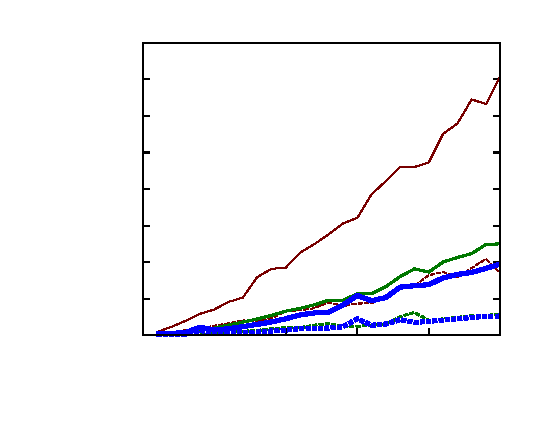
\includegraphics{img/protein}}%
    \gplfronttext
  \end{picture}%
\endgroup
}
{% GNUPLOT: LaTeX picture with Postscript
\begingroup
  \makeatletter
  \providecommand\color[2][]{%
    \GenericError{(gnuplot) \space\space\space\@spaces}{%
      Package color not loaded in conjunction with
      terminal option `colourtext'%
    }{See the gnuplot documentation for explanation.%
    }{Either use 'blacktext' in gnuplot or load the package
      color.sty in LaTeX.}%
    \renewcommand\color[2][]{}%
  }%
  \providecommand\includegraphics[2][]{%
    \GenericError{(gnuplot) \space\space\space\@spaces}{%
      Package graphicx or graphics not loaded%
    }{See the gnuplot documentation for explanation.%
    }{The gnuplot epslatex terminal needs graphicx.sty or graphics.sty.}%
    \renewcommand\includegraphics[2][]{}%
  }%
  \providecommand\rotatebox[2]{#2}%
  \@ifundefined{ifGPcolor}{%
    \newif\ifGPcolor
    \GPcolortrue
  }{}%
  \@ifundefined{ifGPblacktext}{%
    \newif\ifGPblacktext
    \GPblacktextfalse
  }{}%
  % define a \g@addto@macro without @ in the name:
  \let\gplgaddtomacro\g@addto@macro
  % define empty templates for all commands taking text:
  \gdef\gplbacktext{}%
  \gdef\gplfronttext{}%
  \makeatother
  \ifGPblacktext
    % no textcolor at all
    \def\colorrgb#1{}%
    \def\colorgray#1{}%
  \else
    % gray or color?
    \ifGPcolor
      \def\colorrgb#1{\color[rgb]{#1}}%
      \def\colorgray#1{\color[gray]{#1}}%
      \expandafter\def\csname LTw\endcsname{\color{white}}%
      \expandafter\def\csname LTb\endcsname{\color{black}}%
      \expandafter\def\csname LTa\endcsname{\color{black}}%
      \expandafter\def\csname LT0\endcsname{\color[rgb]{1,0,0}}%
      \expandafter\def\csname LT1\endcsname{\color[rgb]{0,1,0}}%
      \expandafter\def\csname LT2\endcsname{\color[rgb]{0,0,1}}%
      \expandafter\def\csname LT3\endcsname{\color[rgb]{1,0,1}}%
      \expandafter\def\csname LT4\endcsname{\color[rgb]{0,1,1}}%
      \expandafter\def\csname LT5\endcsname{\color[rgb]{1,1,0}}%
      \expandafter\def\csname LT6\endcsname{\color[rgb]{0,0,0}}%
      \expandafter\def\csname LT7\endcsname{\color[rgb]{1,0.3,0}}%
      \expandafter\def\csname LT8\endcsname{\color[rgb]{0.5,0.5,0.5}}%
    \else
      % gray
      \def\colorrgb#1{\color{black}}%
      \def\colorgray#1{\color[gray]{#1}}%
      \expandafter\def\csname LTw\endcsname{\color{white}}%
      \expandafter\def\csname LTb\endcsname{\color{black}}%
      \expandafter\def\csname LTa\endcsname{\color{black}}%
      \expandafter\def\csname LT0\endcsname{\color{black}}%
      \expandafter\def\csname LT1\endcsname{\color{black}}%
      \expandafter\def\csname LT2\endcsname{\color{black}}%
      \expandafter\def\csname LT3\endcsname{\color{black}}%
      \expandafter\def\csname LT4\endcsname{\color{black}}%
      \expandafter\def\csname LT5\endcsname{\color{black}}%
      \expandafter\def\csname LT6\endcsname{\color{black}}%
      \expandafter\def\csname LT7\endcsname{\color{black}}%
      \expandafter\def\csname LT8\endcsname{\color{black}}%
    \fi
  \fi
  \setlength{\unitlength}{0.0500bp}%
  \begin{picture}(5040.00,3772.00)%
    \gplgaddtomacro\gplbacktext{%
      \csname LTb\endcsname%
      \put(1078,704){\makebox(0,0)[r]{\strut{} 0}}%
      \put(1078,1054){\makebox(0,0)[r]{\strut{} 200}}%
      \put(1078,1405){\makebox(0,0)[r]{\strut{} 400}}%
      \put(1078,1755){\makebox(0,0)[r]{\strut{} 600}}%
      \put(1078,2106){\makebox(0,0)[r]{\strut{} 800}}%
      \put(1078,2456){\makebox(0,0)[r]{\strut{} 1000}}%
      \put(1078,2806){\makebox(0,0)[r]{\strut{} 1200}}%
      \put(1078,3157){\makebox(0,0)[r]{\strut{} 1400}}%
      \put(1078,3507){\makebox(0,0)[r]{\strut{} 1600}}%
      \put(1210,484){\makebox(0,0){\strut{} 0}}%
      \put(1897,484){\makebox(0,0){\strut{} 50}}%
      \put(2583,484){\makebox(0,0){\strut{} 100}}%
      \put(3270,484){\makebox(0,0){\strut{} 150}}%
      \put(3956,484){\makebox(0,0){\strut{} 200}}%
      \put(4643,484){\makebox(0,0){\strut{} 250}}%
      \put(176,2105){\rotatebox{-270}{\makebox(0,0){\strut{}total distance comparisons (millions)}}}%
      \put(2926,154){\makebox(0,0){\strut{}number of data points (thousands)}}%
    }%
    \gplgaddtomacro\gplfronttext{%
    }%
    \gplbacktext
    \put(0,0){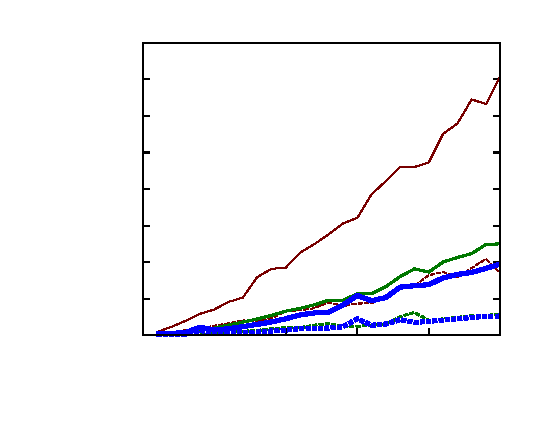
\includegraphics{img/protein}}%
    \gplfronttext
  \end{picture}%
\endgroup
}

%\vspace{0.2in}

\begin{tikzpicture}
\small
%\draw (-3.7,0.5) to (4.4,0.5) to (4.4,-2) to (-3.7,-2) to (-3.7,0.5);
\node at (-2,0) {original c.t.};
\draw[red,dotted] (0,0) to (1.8,0);
\draw[red] (2.3,0) to (4.1,0);

\node at (-2,-0.35) {simplified c.t.};
\draw[darkgreen,dotted,line width=1pt] (0,-0.35) to (1.8,-0.35);
\draw[darkgreen,line width=1pt] (2.3,-0.35) to (4.1,-0.35);

\node at (-2,-0.7) {nearest ancestor c.t.};
\draw[blue,dotted,line width=2pt] (0,-0.7) to (1.8,-0.7);
\draw[blue,line width=2pt] (2.3,-0.7) to (4.1,-0.7);

\node[align=center] at (0.9,-1.2) { construction \\ only };
\node[align=center] at (3.2,-1.2) {construction \\ and query };
\end{tikzpicture}
%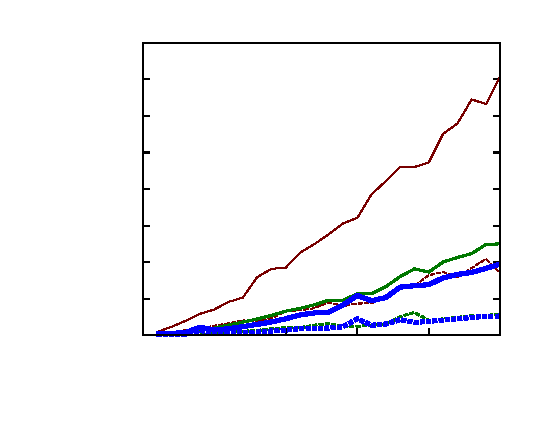
\includegraphics[width=9cm,height=6cm]{img/protein}
\caption{
%Number of distance comparisons versus the number of proteins, for finding all nearest neighbors.
The effect on runtime as we increase the number of data points on the bionformatics data.
The relationship is roughly linear, indicating protein graphs have a relatively low intrinsic dimensionality. % and work well with cover trees.
%On our protein graph dataset, the number of distance comparisons scales roughly linearly with the number of graphs.
%This indicates that protein graphs have a relatively low intrinsic dimensionality and are particularly well suited for use with cover trees.
As expected, the nearest ancestor cover tree performs the best.
    %This figure shows how performance on our protein data scales according to the size of the dataset.
%The thin red line (
%\begin{tikzpicture}
%\draw[color=red,line width=0.5pt] (0,0) -- (0.5,0);
%\node (0,0.1) {};
%\end{tikzpicture}
%) is the original cover tree;
%the medium green line (
%\begin{tikzpicture}
%\draw[color=green,line width=1pt] (0,0) -- (0.5,0);
%\node (0,0.1) {};
%\end{tikzpicture}
%) is the simplified cover tree;
%the thick blue line (
%\begin{tikzpicture}
%\draw[color=blue,line width=2pt] (0,0) -- (0.5,0);
%\node (0,0.1) {};
%\end{tikzpicture}
%) is the ancestor cover tree.
%Dashed lines indicate tree construction time and solid lines indicate total time for both construction and querying
    }
\label{fig:bio}
\end{figure}

\subsection{Earth mover's distance}

%The Earth Mover's Distance (EMD) is a distance metric between histograms.
%It was developed specifically for image classification problems \cite{Rubner1998}.
The Earth Mover's Distance (EMD) is a distance metric between histograms designed for image classification \cite{Rubner1998}.
In our tests, we convert images into three dimensional histograms of the pixel values in LabCIE color space.
LabCIE is a color space represents colors in three dimensions.
It is similar to the more familiar RGB and CMYK color spaces,
but the distances between colors more accurately match what humans perceive color distances to be.
We construct the histogram such that each dimension has 8 equally spaced intervals, for a total of 512 bins.
We then create a ``signature'' of the histogram by recording only the 20 largest of the 512 bins.

Previous research on speeding up EMD focused on computing EMD distances faster.
The EMD takes a base distance as a parameter.
For an arbitrary base distance, EMD requires $O(b^3\log b)$ time where $b$ is the size of the histogram signature.
Faster algorithms exist for specific base metrics.
For example, with an $L_1$ base metric the EMD can be computed in time $O(b^2)$ \citep{Ling07}; and if the base metric is a so-called ``thresholded metric,'' we can get an order of magnitude constant factor speed up \citep{Pele2009}.
We specifically chose the LabCIE color space because there is no known faster EMD algorithm.
It will stress-test our cover tree implementation.

In this experiment, we use the Yahoo! Flickr Creative Commons dataset.
The dataset contains 1.5 million images in its training set,
and we construct simplified and nearest ancestor cover trees in parallel on this data.
Construction times are shown in Table \ref{tab:emd}.
Using the cheap L2 distance with smaller datasets, tree construction happens quickly and so parallelization is less important.
But with an expensive distance on this larger dataset, parallel construction makes a big difference.

\begin{table}
\centering
%\resizebox{\columnwidth}{!}{
\begin{tabular}{ccccc}
%\hline
\multirow{3}{*}{\parbox{1cm}{\centering number of cores}}
 & \multicolumn{2}{c}{simplified tree} & \multicolumn{2}{c}{nearest ancestor tree} \\
& \multicolumn{2}{c}{construction} & \multicolumn{2}{c}{construction} \\ %\cline{2-5}
& time & speedup & time & speedup \\
\hline
%\hline
1  & 70.7 min & 1.0 & 210.9 min& 1.0\\
2  & 36.6 min & 1.9 & 94.2 min & 2.2\\
4  & 18.5 min & 3.8 & 48.5 min & 4.3\\
8  & 10.2 min & 6.9 & 25.3 min & 8.3\\
16 & 6.7 min & 10.5 & 12.0 min & 17.6\\
%\hline
\end{tabular}
%}
\caption{
    Parallel cover tree construction using the earth movers distance.
    On this large dataset with an expensive metric, we see better parallel speedup than on the datasets with the cheaper L2 metric.
The nearest ancestor cover tree gets super-linear parallel speedup because we are merging with Algorithm \ref{alg:merge}, which does not attempt to rebalance.
}
\label{tab:emd}
\end{table}

%%%%%%%%%%%%%%%%%%%%%%%%%%%%%%%%%%%%%%%%%%%%%%%%%%%%%%%%%%%%%%%%%%%%%%%%%%%%%%%%
\bibliography{bibfile}

\end{document}
